\documentclass[twoside]{book}

% Packages required by doxygen
\usepackage{fixltx2e}
\usepackage{calc}
\usepackage{doxygen}
\usepackage[export]{adjustbox} % also loads graphicx
\usepackage{graphicx}
\usepackage[utf8]{inputenc}
\usepackage{makeidx}
\usepackage{multicol}
\usepackage{multirow}
\PassOptionsToPackage{warn}{textcomp}
\usepackage{textcomp}
\usepackage[nointegrals]{wasysym}
\usepackage[table]{xcolor}

% Font selection
\usepackage[T1]{fontenc}
\usepackage[scaled=.90]{helvet}
\usepackage{courier}
\usepackage{amssymb}
\usepackage{sectsty}
\renewcommand{\familydefault}{\sfdefault}
\allsectionsfont{%
  \fontseries{bc}\selectfont%
  \color{darkgray}%
}
\renewcommand{\DoxyLabelFont}{%
  \fontseries{bc}\selectfont%
  \color{darkgray}%
}
\newcommand{\+}{\discretionary{\mbox{\scriptsize$\hookleftarrow$}}{}{}}

% Page & text layout
\usepackage{geometry}
\geometry{%
  a4paper,%
  top=2.5cm,%
  bottom=2.5cm,%
  left=2.5cm,%
  right=2.5cm%
}
\tolerance=750
\hfuzz=15pt
\hbadness=750
\setlength{\emergencystretch}{15pt}
\setlength{\parindent}{0cm}
\setlength{\parskip}{3ex plus 2ex minus 2ex}
\makeatletter
\renewcommand{\paragraph}{%
  \@startsection{paragraph}{4}{0ex}{-1.0ex}{1.0ex}{%
    \normalfont\normalsize\bfseries\SS@parafont%
  }%
}
\renewcommand{\subparagraph}{%
  \@startsection{subparagraph}{5}{0ex}{-1.0ex}{1.0ex}{%
    \normalfont\normalsize\bfseries\SS@subparafont%
  }%
}
\makeatother

% Headers & footers
\usepackage{fancyhdr}
\pagestyle{fancyplain}
\fancyhead[LE]{\fancyplain{}{\bfseries\thepage}}
\fancyhead[CE]{\fancyplain{}{}}
\fancyhead[RE]{\fancyplain{}{\bfseries\leftmark}}
\fancyhead[LO]{\fancyplain{}{\bfseries\rightmark}}
\fancyhead[CO]{\fancyplain{}{}}
\fancyhead[RO]{\fancyplain{}{\bfseries\thepage}}
\fancyfoot[LE]{\fancyplain{}{}}
\fancyfoot[CE]{\fancyplain{}{}}
\fancyfoot[RE]{\fancyplain{}{\bfseries\scriptsize Generated by Doxygen }}
\fancyfoot[LO]{\fancyplain{}{\bfseries\scriptsize Generated by Doxygen }}
\fancyfoot[CO]{\fancyplain{}{}}
\fancyfoot[RO]{\fancyplain{}{}}
\renewcommand{\footrulewidth}{0.4pt}
\renewcommand{\chaptermark}[1]{%
  \markboth{#1}{}%
}
\renewcommand{\sectionmark}[1]{%
  \markright{\thesection\ #1}%
}

% Indices & bibliography
\usepackage{natbib}
\usepackage[titles]{tocloft}
\setcounter{tocdepth}{3}
\setcounter{secnumdepth}{5}
\makeindex

% Hyperlinks (required, but should be loaded last)
\usepackage{ifpdf}
\ifpdf
  \usepackage[pdftex,pagebackref=true]{hyperref}
\else
  \usepackage[ps2pdf,pagebackref=true]{hyperref}
\fi
\hypersetup{%
  colorlinks=true,%
  linkcolor=blue,%
  citecolor=blue,%
  unicode%
}

% Custom commands
\newcommand{\clearemptydoublepage}{%
  \newpage{\pagestyle{empty}\cleardoublepage}%
}

\usepackage{caption}
\captionsetup{labelsep=space,justification=centering,font={bf},singlelinecheck=off,skip=4pt,position=top}

%===== C O N T E N T S =====

\begin{document}

% Titlepage & ToC
\hypersetup{pageanchor=false,
             bookmarksnumbered=true,
             pdfencoding=unicode
            }
\pagenumbering{roman}
\begin{titlepage}
\vspace*{7cm}
\begin{center}%
{\Large pf }\\
\vspace*{1cm}
{\large Generated by Doxygen 1.8.11}\\
\end{center}
\end{titlepage}
\clearemptydoublepage
\tableofcontents
\clearemptydoublepage
\pagenumbering{arabic}
\hypersetup{pageanchor=true}

%--- Begin generated contents ---
\chapter{PF\+: a library for fast particle filtering!}
\label{index}\hypertarget{index}{}\href{https://zenodo.org/badge/latestdoi/130237492}{\tt }

This is a template library for fast particle filtering. Templated abstract base classes for different particle filters are provided (e.\+g. the Bootstrap Filter, the Auxiliary Particle Filter, Rao-\/\+Blackwellized particle filter, etc.), as well as non-\/abstract (but indeed templated) base classes for closed form filtering algorithms (e.\+g. Kalman Filter, Hidden Markov Model filter, etc.).

Once you have a certain model in mind, all you have to do is make it into a class that inherits from the filter you want to use!

\subsection*{Installation}

This is a header-\/only library, so there is no building necessary. When you use it in another project, make sure to compile with C++11 enabled ({\ttfamily -\/std=c++11}), and to include the {\ttfamily include} directory of this project.

Note, also, that this code all makes use of \href{http://eigen.tuxfamily.org/}{\tt Eigen} and \href{https://www.boost.org/}{\tt Boost}.

\subsection*{Examples}

Don\textquotesingle{}t know how to use this? Check out the \href{https://github.com/tbrown122387/pf/tree/master/examples}{\tt {\ttfamily examples}} directory! Check {\ttfamily pf/examples/\+Makefile} to make sure it jives with your directories, and then run {\ttfamily make}. After that, run {\ttfamily ./examples ./data/svol\+\_\+y\+\_\+data.csv} and you\textquotesingle{}ll see the filtering output from {\ttfamily examples/svol\+\_\+comparison.\+cpp}.

\subsection*{Citation}

Click the \char`\"{}\+D\+O\+I\char`\"{} link above. Or, if you\textquotesingle{}re impatient, click \href{https://zenodo.org/record/2633289/export/hx}{\tt \textquotesingle{}here\textquotesingle{}} for a Bibtex citation. 
\chapter{Todo List}
\label{todo}
\hypertarget{todo}{}

\begin{DoxyRefList}
\item[\label{todo__todo000001}%
\Hypertarget{todo__todo000001}%
Member \hyperlink{classBSFilter_a651d0228e8477c0ca7d522cd72908a57}{B\+S\+Filter$<$ nparts, dimx, dimy, resamp\+\_\+t, float\+\_\+t $>$\+:\+:filter} (const osv \&data, const std\+::vector$<$ std\+::function$<$ const Mat(const ssv \&)$>$ $>$ \&fs=std\+::vector$<$ std\+::function$<$ const Mat(const ssv \&)$>$ $>$())]\+: work in support for effective sample size stuff.  
\item[\label{todo__todo000002}%
\Hypertarget{todo__todo000002}%
Member \hyperlink{classBSFilterWC_a0637035a4553ae3ffeaf1ddce0de2c6b}{B\+S\+Filter\+WC$<$ nparts, dimx, dimy, dimcov, resamp\+\_\+t, float\+\_\+t $>$\+:\+:filter} (const osv \&ydata, const cvsv \&covdata, const std\+::vector$<$ std\+::function$<$ const Mat(const ssv \&)$>$ $>$ \&fs=std\+::vector$<$ std\+::function$<$ const Mat(const ssv \&)$>$ $>$())]\+: work in support for effective sample size stuff.  
\item[\label{todo__todo000003}%
\Hypertarget{todo__todo000003}%
Member \hyperlink{classkalman_af4a5d62ffbd478fedfb040cb9e4fcb24}{kalman$<$ dimstate, dimobs, diminput, float\+\_\+t $>$\+:\+:update\+Prior} (const ss\+Mat \&state\+Trans\+Mat, const ss\+Mat \&chol\+State\+Var, const si\+Mat \&state\+Inpt\+Affector, const isv \&input\+Data)]handle diagonal variance matrices, and ensure symmetricness in other ways  
\item[\label{todo__todo000004}%
\Hypertarget{todo__todo000004}%
Member \hyperlink{classrvsamp_1_1MVNSampler_a5fa6029b9bd840c4b08a01f67a97afc6}{rvsamp\+:\+:M\+V\+N\+Sampler$<$ dim, float\+\_\+t $>$\+:\+:M\+V\+N\+Sampler} ()]\+: implement move semantics 
\end{DoxyRefList}
\chapter{Hierarchical Index}
\section{Class Hierarchy}
This inheritance list is sorted roughly, but not completely, alphabetically\+:\begin{DoxyCompactList}
\item \contentsline{section}{B\+S\+Filter\+WC$<$ nparts, dimx, dimy, dimcov, resamp\+\_\+t, float\+\_\+t $>$}{\pageref{classBSFilterWC}}{}
\item \contentsline{section}{cf\+\_\+filter$<$ dimstate, dimobs, float\+\_\+t $>$}{\pageref{classcf__filter}}{}
\begin{DoxyCompactList}
\item \contentsline{section}{hmm$<$ dimstate, dimobs, float\+\_\+t $>$}{\pageref{classhmm}}{}
\item \contentsline{section}{kalman$<$ dimstate, dimobs, diminput, float\+\_\+t $>$}{\pageref{classkalman}}{}
\end{DoxyCompactList}
\item \contentsline{section}{cf\+\_\+filter$<$ 1, 1, float\+\_\+t $>$}{\pageref{classcf__filter}}{}
\begin{DoxyCompactList}
\item \contentsline{section}{gam\+Filter$<$ dim\+\_\+pred, float\+\_\+t $>$}{\pageref{classgamFilter}}{}
\end{DoxyCompactList}
\item \contentsline{section}{cf\+\_\+filter$<$ 1, dim\+\_\+obs, float\+\_\+t $>$}{\pageref{classcf__filter}}{}
\begin{DoxyCompactList}
\item \contentsline{section}{multiv\+Gam\+Filter$<$ dim\+\_\+obs, dim\+\_\+pred, float\+\_\+t $>$}{\pageref{classmultivGamFilter}}{}
\end{DoxyCompactList}
\item \contentsline{section}{Forward\+Mod$<$ dimx, dimy, float\+\_\+t $>$}{\pageref{classForwardMod}}{}
\item \contentsline{section}{mn\+\_\+resampler\+\_\+rbpf$<$ nparts, dimsampledx, cf\+ModT, float\+\_\+t $>$}{\pageref{classmn__resampler__rbpf}}{}
\item \contentsline{section}{pf\+\_\+base$<$ float\+\_\+t, dimobs, dimstate $>$}{\pageref{classpf__base}}{}
\item \contentsline{section}{pf\+\_\+base$<$ float\+\_\+t, dimy, dimx $>$}{\pageref{classpf__base}}{}
\begin{DoxyCompactList}
\item \contentsline{section}{A\+PF$<$ nparts, dimx, dimy, resamp\+\_\+t, float\+\_\+t, debug $>$}{\pageref{classAPF}}{}
\item \contentsline{section}{B\+S\+Filter$<$ nparts, dimx, dimy, resamp\+\_\+t, float\+\_\+t, debug $>$}{\pageref{classBSFilter}}{}
\item \contentsline{section}{S\+I\+S\+R\+Filter$<$ nparts, dimx, dimy, resamp\+\_\+t, float\+\_\+t, debug $>$}{\pageref{classSISRFilter}}{}
\end{DoxyCompactList}
\item \contentsline{section}{rbase$<$ nparts, dimx, float\+\_\+t $>$}{\pageref{classrbase}}{}
\begin{DoxyCompactList}
\item \contentsline{section}{mn\+\_\+resamp\+\_\+fast1$<$ nparts, dimx, float\+\_\+t $>$}{\pageref{classmn__resamp__fast1}}{}
\item \contentsline{section}{mn\+\_\+resampler$<$ nparts, dimx, float\+\_\+t $>$}{\pageref{classmn__resampler}}{}
\item \contentsline{section}{resid\+\_\+resampler$<$ nparts, dimx, float\+\_\+t $>$}{\pageref{classresid__resampler}}{}
\item \contentsline{section}{stratif\+\_\+resampler$<$ nparts, dimx, float\+\_\+t $>$}{\pageref{classstratif__resampler}}{}
\item \contentsline{section}{systematic\+\_\+resampler$<$ nparts, dimx, float\+\_\+t $>$}{\pageref{classsystematic__resampler}}{}
\end{DoxyCompactList}
\item \contentsline{section}{rbpf\+\_\+base$<$ float\+\_\+t, dim\+\_\+s\+\_\+state, dim\+\_\+ns\+\_\+state, dimobs $>$}{\pageref{classrbpf__base}}{}
\item \contentsline{section}{rbpf\+\_\+base$<$ float\+\_\+t, dimss, dimnss, dimy $>$}{\pageref{classrbpf__base}}{}
\begin{DoxyCompactList}
\item \contentsline{section}{rbpf\+\_\+hmm$<$ nparts, dimnss, dimss, dimy, resamp\+\_\+t, float\+\_\+t $>$}{\pageref{classrbpf__hmm}}{}
\item \contentsline{section}{rbpf\+\_\+hmm\+\_\+bs$<$ nparts, dimnss, dimss, dimy, resamp\+\_\+t, float\+\_\+t $>$}{\pageref{classrbpf__hmm__bs}}{}
\item \contentsline{section}{rbpf\+\_\+kalman$<$ nparts, dimnss, dimss, dimy, resamp\+\_\+t, float\+\_\+t $>$}{\pageref{classrbpf__kalman}}{}
\item \contentsline{section}{rbpf\+\_\+kalman\+\_\+bs$<$ nparts, dimnss, dimss, dimy, resamp\+\_\+t, float\+\_\+t $>$}{\pageref{classrbpf__kalman__bs}}{}
\end{DoxyCompactList}
\item \contentsline{section}{rvsamp\+:\+:rvsamp\+\_\+base}{\pageref{classrvsamp_1_1rvsamp__base}}{}
\begin{DoxyCompactList}
\item \contentsline{section}{rvsamp\+:\+:k\+\_\+gen$<$ nparts, float\+\_\+t $>$}{\pageref{classrvsamp_1_1k__gen}}{}
\item \contentsline{section}{rvsamp\+:\+:Bern\+Sampler$<$ float\+\_\+t, int\+\_\+t $>$}{\pageref{classrvsamp_1_1BernSampler}}{}
\item \contentsline{section}{rvsamp\+:\+:k\+\_\+gen$<$ N, float\+\_\+t $>$}{\pageref{classrvsamp_1_1k__gen}}{}
\item \contentsline{section}{rvsamp\+:\+:M\+V\+N\+Sampler$<$ dim, float\+\_\+t $>$}{\pageref{classrvsamp_1_1MVNSampler}}{}
\item \contentsline{section}{rvsamp\+:\+:Poisson\+Sampler$<$ float\+\_\+t, int\+\_\+t $>$}{\pageref{classrvsamp_1_1PoissonSampler}}{}
\item \contentsline{section}{rvsamp\+:\+:Trunc\+Univ\+Norm\+Sampler$<$ float\+\_\+t $>$}{\pageref{classrvsamp_1_1TruncUnivNormSampler}}{}
\item \contentsline{section}{rvsamp\+:\+:Uniform\+Sampler$<$ float\+\_\+t $>$}{\pageref{classrvsamp_1_1UniformSampler}}{}
\item \contentsline{section}{rvsamp\+:\+:Univ\+Gamma\+Sampler$<$ float\+\_\+t $>$}{\pageref{classrvsamp_1_1UnivGammaSampler}}{}
\item \contentsline{section}{rvsamp\+:\+:Univ\+Inv\+Gamma\+Sampler$<$ float\+\_\+t $>$}{\pageref{classrvsamp_1_1UnivInvGammaSampler}}{}
\item \contentsline{section}{rvsamp\+:\+:Univ\+Log\+Norm\+Sampler$<$ float\+\_\+t $>$}{\pageref{classrvsamp_1_1UnivLogNormSampler}}{}
\item \contentsline{section}{rvsamp\+:\+:Univ\+Norm\+Sampler$<$ float\+\_\+t $>$}{\pageref{classrvsamp_1_1UnivNormSampler}}{}
\end{DoxyCompactList}
\end{DoxyCompactList}

\chapter{Class Index}
\section{Class List}
Here are the classes, structs, unions and interfaces with brief descriptions\+:\begin{DoxyCompactList}
\item\contentsline{section}{\hyperlink{classAPF}{A\+P\+F$<$ nparts, dimx, dimy, resamp\+\_\+t, float\+\_\+t, debug $>$} \\*A base-\/class for Auxiliary Particle Filtering. Filtering only, no smoothing }{\pageref{classAPF}}{}
\item\contentsline{section}{\hyperlink{classrvsamp_1_1BernSampler}{rvsamp\+::\+Bern\+Sampler$<$ float\+\_\+t, int\+\_\+t $>$} \\*A class that performs sampling from a univariate Bernoulli distribution }{\pageref{classrvsamp_1_1BernSampler}}{}
\item\contentsline{section}{\hyperlink{classBSFilter}{B\+S\+Filter$<$ nparts, dimx, dimy, resamp\+\_\+t, float\+\_\+t, debug $>$} \\*A base class for the bootstrap particle filter }{\pageref{classBSFilter}}{}
\item\contentsline{section}{\hyperlink{classBSFilterWC}{B\+S\+Filter\+W\+C$<$ nparts, dimx, dimy, dimcov, resamp\+\_\+t, float\+\_\+t $>$} \\*A base class for the bootstrap particle filter with covariates }{\pageref{classBSFilterWC}}{}
\item\contentsline{section}{\hyperlink{classcf__filter}{cf\+\_\+filter$<$ dimstate, dimobs, float\+\_\+t $>$} \\*Abstract Base Class for all closed-\/form filters }{\pageref{classcf__filter}}{}
\item\contentsline{section}{\hyperlink{classForwardMod}{Forward\+Mod$<$ dimx, dimy, float\+\_\+t $>$} }{\pageref{classForwardMod}}{}
\item\contentsline{section}{\hyperlink{classgamFilter}{gam\+Filter$<$ dim\+\_\+pred, float\+\_\+t $>$} \\*A class template for Gamma filtering }{\pageref{classgamFilter}}{}
\item\contentsline{section}{\hyperlink{classhmm}{hmm$<$ dimstate, dimobs, float\+\_\+t $>$} \\*A class template for H\+MM filtering }{\pageref{classhmm}}{}
\item\contentsline{section}{\hyperlink{classrvsamp_1_1k__gen}{rvsamp\+::k\+\_\+gen$<$ N, float\+\_\+t $>$} \\*A class that performs sampling with replacement (useful for the index sampler in an \hyperlink{classAPF}{A\+PF}) }{\pageref{classrvsamp_1_1k__gen}}{}
\item\contentsline{section}{\hyperlink{classkalman}{kalman$<$ dimstate, dimobs, diminput, float\+\_\+t $>$} \\*A class template for Kalman filtering }{\pageref{classkalman}}{}
\item\contentsline{section}{\hyperlink{classmn__resamp__fast1}{mn\+\_\+resamp\+\_\+fast1$<$ nparts, dimx, float\+\_\+t $>$} }{\pageref{classmn__resamp__fast1}}{}
\item\contentsline{section}{\hyperlink{classmn__resampler}{mn\+\_\+resampler$<$ nparts, dimx, float\+\_\+t $>$} }{\pageref{classmn__resampler}}{}
\item\contentsline{section}{\hyperlink{classmn__resampler__rbpf}{mn\+\_\+resampler\+\_\+rbpf$<$ nparts, dimsampledx, cf\+Mod\+T, float\+\_\+t $>$} }{\pageref{classmn__resampler__rbpf}}{}
\item\contentsline{section}{\hyperlink{classmultivGamFilter}{multiv\+Gam\+Filter$<$ dim\+\_\+obs, dim\+\_\+pred, float\+\_\+t $>$} \\*Another class template for Gamma filtering, but this time }{\pageref{classmultivGamFilter}}{}
\item\contentsline{section}{\hyperlink{classrvsamp_1_1MVNSampler}{rvsamp\+::\+M\+V\+N\+Sampler$<$ dim, float\+\_\+t $>$} \\*A class that performs sampling from a multivariate normal distribution }{\pageref{classrvsamp_1_1MVNSampler}}{}
\item\contentsline{section}{\hyperlink{classpf__base}{pf\+\_\+base$<$ float\+\_\+t, dimobs, dimstate $>$} }{\pageref{classpf__base}}{}
\item\contentsline{section}{\hyperlink{classrvsamp_1_1PoissonSampler}{rvsamp\+::\+Poisson\+Sampler$<$ float\+\_\+t, int\+\_\+t $>$} \\*A class that performs sampling from a Poisson distribution }{\pageref{classrvsamp_1_1PoissonSampler}}{}
\item\contentsline{section}{\hyperlink{classrbase}{rbase$<$ nparts, dimx, float\+\_\+t $>$} \\*Base class for all resampler types }{\pageref{classrbase}}{}
\item\contentsline{section}{\hyperlink{classrbpf__base}{rbpf\+\_\+base$<$ float\+\_\+t, dim\+\_\+s\+\_\+state, dim\+\_\+ns\+\_\+state, dimobs $>$} }{\pageref{classrbpf__base}}{}
\item\contentsline{section}{\hyperlink{classrbpf__hmm}{rbpf\+\_\+hmm$<$ nparts, dimnss, dimss, dimy, resamp\+\_\+t, float\+\_\+t $>$} \\*Rao-\/\+Blackwellized/\+Marginal Particle Filter with inner H\+M\+Ms }{\pageref{classrbpf__hmm}}{}
\item\contentsline{section}{\hyperlink{classrbpf__hmm__bs}{rbpf\+\_\+hmm\+\_\+bs$<$ nparts, dimnss, dimss, dimy, resamp\+\_\+t, float\+\_\+t $>$} \\*Rao-\/\+Blackwellized/\+Marginal Bootstrap Filter with inner H\+M\+Ms }{\pageref{classrbpf__hmm__bs}}{}
\item\contentsline{section}{\hyperlink{classrbpf__kalman}{rbpf\+\_\+kalman$<$ nparts, dimnss, dimss, dimy, resamp\+\_\+t, float\+\_\+t $>$} \\*Rao-\/\+Blackwellized/\+Marginal Particle Filter with inner Kalman Filter objectss }{\pageref{classrbpf__kalman}}{}
\item\contentsline{section}{\hyperlink{classrbpf__kalman__bs}{rbpf\+\_\+kalman\+\_\+bs$<$ nparts, dimnss, dimss, dimy, resamp\+\_\+t, float\+\_\+t $>$} \\*Rao-\/\+Blackwellized/\+Marginal Bootstrap Filter with inner Kalman Filter objectss }{\pageref{classrbpf__kalman__bs}}{}
\item\contentsline{section}{\hyperlink{classresid__resampler}{resid\+\_\+resampler$<$ nparts, dimx, float\+\_\+t $>$} }{\pageref{classresid__resampler}}{}
\item\contentsline{section}{\hyperlink{classrvsamp_1_1rvsamp__base}{rvsamp\+::rvsamp\+\_\+base} \\*Base class for all random variable sampler types. Primary benefit is that it sets the seed for you }{\pageref{classrvsamp_1_1rvsamp__base}}{}
\item\contentsline{section}{\hyperlink{classSISRFilter}{S\+I\+S\+R\+Filter$<$ nparts, dimx, dimy, resamp\+\_\+t, float\+\_\+t, debug $>$} \\*A base class for the Sequential Important Sampling with Resampling (S\+I\+SR) }{\pageref{classSISRFilter}}{}
\item\contentsline{section}{\hyperlink{classstratif__resampler}{stratif\+\_\+resampler$<$ nparts, dimx, float\+\_\+t $>$} }{\pageref{classstratif__resampler}}{}
\item\contentsline{section}{\hyperlink{classsystematic__resampler}{systematic\+\_\+resampler$<$ nparts, dimx, float\+\_\+t $>$} }{\pageref{classsystematic__resampler}}{}
\item\contentsline{section}{\hyperlink{classrvsamp_1_1TruncUnivNormSampler}{rvsamp\+::\+Trunc\+Univ\+Norm\+Sampler$<$ float\+\_\+t $>$} \\*A class that performs sampling from a truncated univariate Normal distribution }{\pageref{classrvsamp_1_1TruncUnivNormSampler}}{}
\item\contentsline{section}{\hyperlink{classrvsamp_1_1UniformSampler}{rvsamp\+::\+Uniform\+Sampler$<$ float\+\_\+t $>$} \\*A class that performs sampling from a continuous uniform distribution }{\pageref{classrvsamp_1_1UniformSampler}}{}
\item\contentsline{section}{\hyperlink{classrvsamp_1_1UnivGammaSampler}{rvsamp\+::\+Univ\+Gamma\+Sampler$<$ float\+\_\+t $>$} \\*A class that performs sampling from a univariate Gamma distribution }{\pageref{classrvsamp_1_1UnivGammaSampler}}{}
\item\contentsline{section}{\hyperlink{classrvsamp_1_1UnivInvGammaSampler}{rvsamp\+::\+Univ\+Inv\+Gamma\+Sampler$<$ float\+\_\+t $>$} \\*A class that performs sampling from a univariate Inverse Gamma distribution }{\pageref{classrvsamp_1_1UnivInvGammaSampler}}{}
\item\contentsline{section}{\hyperlink{classrvsamp_1_1UnivLogNormSampler}{rvsamp\+::\+Univ\+Log\+Norm\+Sampler$<$ float\+\_\+t $>$} \\*A class that performs sampling from a univariate Log-\/\+Normal distribution }{\pageref{classrvsamp_1_1UnivLogNormSampler}}{}
\item\contentsline{section}{\hyperlink{classrvsamp_1_1UnivNormSampler}{rvsamp\+::\+Univ\+Norm\+Sampler$<$ float\+\_\+t $>$} \\*A class that performs sampling from a univariate Normal distribution }{\pageref{classrvsamp_1_1UnivNormSampler}}{}
\end{DoxyCompactList}

\chapter{File Index}
\section{File List}
Here is a list of all documented files with brief descriptions\+:\begin{DoxyCompactList}
\item\contentsline{section}{include/\hyperlink{auxiliary__pf_8h}{auxiliary\+\_\+pf.\+h} \\*A base class for Auxiliary Particle Filtering. Inherit from this if you want to use an \hyperlink{classAPF}{A\+PF} for your state space model. Filtering only, no smoothing }{\pageref{auxiliary__pf_8h}}{}
\item\contentsline{section}{include/\hyperlink{bootstrap__filter_8h}{bootstrap\+\_\+filter.\+h} \\*Bootstrap particle filter }{\pageref{bootstrap__filter_8h}}{}
\item\contentsline{section}{include/\hyperlink{bootstrap__filter__with__covariates_8h}{bootstrap\+\_\+filter\+\_\+with\+\_\+covariates.\+h} \\*Bootstrap particle filter with covariates }{\pageref{bootstrap__filter__with__covariates_8h}}{}
\item\contentsline{section}{include/\hyperlink{cf__filters_8h}{cf\+\_\+filters.\+h} \\*Forces structure on the closed-\/form filters }{\pageref{cf__filters_8h}}{}
\item\contentsline{section}{include/\hyperlink{pf__base_8h}{pf\+\_\+base.\+h} \\*All particle filters inherit from this }{\pageref{pf__base_8h}}{}
\item\contentsline{section}{include/\hyperlink{rbpf_8h}{rbpf.\+h} \\*Rao-\/\+Blackwellized/\+Marginal Particle Filter with inner H\+M\+Ms }{\pageref{rbpf_8h}}{}
\item\contentsline{section}{include/\hyperlink{resamplers_8h}{resamplers.\+h} \\*All resamplers must inherit from this. This will enforce certain structure that are assumed by all particle filters }{\pageref{resamplers_8h}}{}
\item\contentsline{section}{include/{\bfseries rv\+\_\+eval.\+h} }{\pageref{rv__eval_8h}}{}
\item\contentsline{section}{include/\hyperlink{rv__samp_8h}{rv\+\_\+samp.\+h} \\*All rv samplers must inherit from this }{\pageref{rv__samp_8h}}{}
\item\contentsline{section}{include/\hyperlink{sisr__filter_8h}{sisr\+\_\+filter.\+h} \\*S\+I\+SR filter }{\pageref{sisr__filter_8h}}{}
\item\contentsline{section}{include/{\bfseries utils.\+h} }{\pageref{utils_8h}}{}
\end{DoxyCompactList}

\chapter{Class Documentation}
\hypertarget{classAPF}{}\section{A\+PF$<$ nparts, dimx, dimy, resamp\+\_\+t, float\+\_\+t $>$ Class Template Reference}
\label{classAPF}\index{A\+P\+F$<$ nparts, dimx, dimy, resamp\+\_\+t, float\+\_\+t $>$@{A\+P\+F$<$ nparts, dimx, dimy, resamp\+\_\+t, float\+\_\+t $>$}}


A base-\/class for Auxiliary Particle Filtering. Filtering only, no smoothing.  




{\ttfamily \#include $<$auxiliary\+\_\+pf.\+h$>$}



Inheritance diagram for A\+PF$<$ nparts, dimx, dimy, resamp\+\_\+t, float\+\_\+t $>$\+:\nopagebreak
\begin{figure}[H]
\begin{center}
\leavevmode
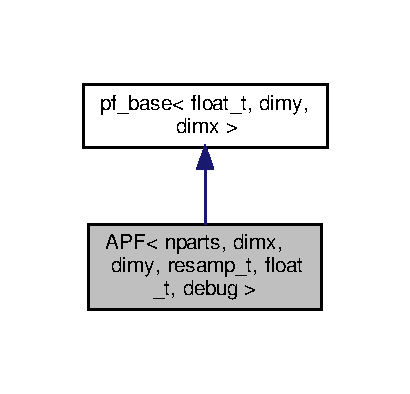
\includegraphics[width=209pt]{classAPF__inherit__graph}
\end{center}
\end{figure}


Collaboration diagram for A\+PF$<$ nparts, dimx, dimy, resamp\+\_\+t, float\+\_\+t $>$\+:\nopagebreak
\begin{figure}[H]
\begin{center}
\leavevmode
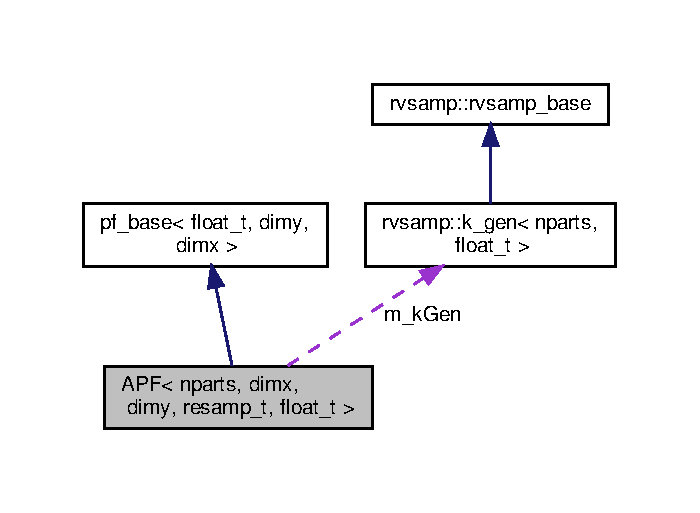
\includegraphics[width=336pt]{classAPF__coll__graph}
\end{center}
\end{figure}
\subsection*{Public Types}
\begin{DoxyCompactItemize}
\item 
using \hyperlink{classAPF_a5f96da87f00ff75af1232f9021daf06a}{ssv} = Eigen\+::\+Matrix$<$ float\+\_\+t, dimx, 1 $>$
\item 
using \hyperlink{classAPF_aa8ac25c475e54ddf21999f28727a049e}{osv} = Eigen\+::\+Matrix$<$ float\+\_\+t, dimy, 1 $>$
\item 
using \hyperlink{classAPF_a448066ff44c8afb24c89bcea11d604c6}{Mat} = Eigen\+::\+Matrix$<$ float\+\_\+t, Eigen\+::\+Dynamic, Eigen\+::\+Dynamic $>$
\item 
using \hyperlink{classAPF_ac686d94dd5c9f06febed3508dad43520}{arrayfloat\+\_\+t} = std\+::array$<$ float\+\_\+t, nparts $>$
\item 
using \hyperlink{classAPF_af0e0643ea340705993c12b1aa7ad0f4d}{array\+Vec} = std\+::array$<$ \hyperlink{classAPF_a5f96da87f00ff75af1232f9021daf06a}{ssv}, nparts $>$
\item 
using \hyperlink{classAPF_a18fed7b33bf9dbb0e3a78b87d1e75272}{array\+U\+Int} = std\+::array$<$ unsigned int, nparts $>$
\end{DoxyCompactItemize}
\subsection*{Public Member Functions}
\begin{DoxyCompactItemize}
\item 
\hyperlink{classAPF_af11ebba0fda9017d21f5d88521584210}{A\+PF} (const unsigned int \&rs=1)
\begin{DoxyCompactList}\small\item\em The constructor. \end{DoxyCompactList}\item 
\mbox{\Hypertarget{classAPF_a5f7a82bbf9d74f93c3d6ebea5f5bf95f}\label{classAPF_a5f7a82bbf9d74f93c3d6ebea5f5bf95f}} 
virtual \hyperlink{classAPF_a5f7a82bbf9d74f93c3d6ebea5f5bf95f}{$\sim$\+A\+PF} ()
\begin{DoxyCompactList}\small\item\em The (virtual) destructor. \end{DoxyCompactList}\item 
float\+\_\+t \hyperlink{classAPF_adc35c009dcf5b3289a4d46279527e024}{get\+Log\+Cond\+Like} () const
\begin{DoxyCompactList}\small\item\em Get the latest log conditional likelihood. \end{DoxyCompactList}\item 
std\+::vector$<$ \hyperlink{classAPF_a448066ff44c8afb24c89bcea11d604c6}{Mat} $>$ \hyperlink{classAPF_a5185ce1aa918dcf176bd0a3ecf6b03dd}{get\+Expectations} () const
\begin{DoxyCompactList}\small\item\em return all stored expectations (taken with respect to \$p(x\+\_\+t$\vert$y\+\_\+\{1\+:t\})\$ \end{DoxyCompactList}\item 
void \hyperlink{classAPF_ab97631b9df8b63e830070604e6887b42}{filter} (const \hyperlink{classAPF_aa8ac25c475e54ddf21999f28727a049e}{osv} \&data, const std\+::vector$<$ std\+::function$<$ const \hyperlink{classAPF_a448066ff44c8afb24c89bcea11d604c6}{Mat}(const \hyperlink{classAPF_a5f96da87f00ff75af1232f9021daf06a}{ssv} \&)$>$ $>$ \&fs=std\+::vector$<$ std\+::function$<$ const \hyperlink{classAPF_a448066ff44c8afb24c89bcea11d604c6}{Mat}(const \hyperlink{classAPF_a5f96da87f00ff75af1232f9021daf06a}{ssv} \&)$>$ $>$())
\begin{DoxyCompactList}\small\item\em Use a new datapoint to update the filtering distribution (or smoothing if path\+Length $>$ 0). \end{DoxyCompactList}\item 
virtual float\+\_\+t \hyperlink{classAPF_a7f595770b8f17cbad8e00b98e1b3bd04}{log\+Mu\+Ev} (const \hyperlink{classAPF_a5f96da87f00ff75af1232f9021daf06a}{ssv} \&x1)=0
\begin{DoxyCompactList}\small\item\em Evaluates the log of mu. \end{DoxyCompactList}\item 
virtual \hyperlink{classAPF_a5f96da87f00ff75af1232f9021daf06a}{ssv} \hyperlink{classAPF_ab57f2f5fb1af1ef6f82fbe1ca3d20905}{prop\+Mu} (const \hyperlink{classAPF_a5f96da87f00ff75af1232f9021daf06a}{ssv} \&xtm1)=0
\begin{DoxyCompactList}\small\item\em Evaluates the proposal distribution taking a Eigen\+::\+Matrix$<$float\+\_\+t,dimx,1$>$ from the previous time\textquotesingle{}s state, and returning a state for the current time. \end{DoxyCompactList}\item 
virtual \hyperlink{classAPF_a5f96da87f00ff75af1232f9021daf06a}{ssv} \hyperlink{classAPF_ad4eaf5c7d00ef9c8b8529e08bda21f13}{q1\+Samp} (const \hyperlink{classAPF_aa8ac25c475e54ddf21999f28727a049e}{osv} \&y1)=0
\begin{DoxyCompactList}\small\item\em Samples from q1. \end{DoxyCompactList}\item 
virtual \hyperlink{classAPF_a5f96da87f00ff75af1232f9021daf06a}{ssv} \hyperlink{classAPF_a30fc3aa6c6217bd4a40f07ee5a9d60d2}{f\+Samp} (const \hyperlink{classAPF_a5f96da87f00ff75af1232f9021daf06a}{ssv} \&xtm1)=0
\begin{DoxyCompactList}\small\item\em Samples from f. \end{DoxyCompactList}\item 
virtual float\+\_\+t \hyperlink{classAPF_aa892fcb9a774cd2158d107cb64f4db49}{log\+Q1\+Ev} (const \hyperlink{classAPF_a5f96da87f00ff75af1232f9021daf06a}{ssv} \&x1, const \hyperlink{classAPF_aa8ac25c475e54ddf21999f28727a049e}{osv} \&y1)=0
\begin{DoxyCompactList}\small\item\em Evaluates the log of q1. \end{DoxyCompactList}\item 
virtual float\+\_\+t \hyperlink{classAPF_ab81a714dacc1ee5ea1aa66ffee46f832}{log\+G\+Ev} (const \hyperlink{classAPF_aa8ac25c475e54ddf21999f28727a049e}{osv} \&yt, const \hyperlink{classAPF_a5f96da87f00ff75af1232f9021daf06a}{ssv} \&xt)=0
\begin{DoxyCompactList}\small\item\em Evaluates the log of g. \end{DoxyCompactList}\end{DoxyCompactItemize}
\subsection*{Protected Attributes}
\begin{DoxyCompactItemize}
\item 
\mbox{\Hypertarget{classAPF_ab1af862a00bf3d1b782b52c8996bf83f}\label{classAPF_ab1af862a00bf3d1b782b52c8996bf83f}} 
std\+::array$<$ \hyperlink{classAPF_a5f96da87f00ff75af1232f9021daf06a}{ssv}, nparts $>$ \hyperlink{classAPF_ab1af862a00bf3d1b782b52c8996bf83f}{m\+\_\+particles}
\begin{DoxyCompactList}\small\item\em particle samples \end{DoxyCompactList}\item 
\mbox{\Hypertarget{classAPF_a23f21a7901654d04256d5aa316afc386}\label{classAPF_a23f21a7901654d04256d5aa316afc386}} 
std\+::array$<$ float\+\_\+t, nparts $>$ \hyperlink{classAPF_a23f21a7901654d04256d5aa316afc386}{m\+\_\+log\+Un\+Norm\+Weights}
\begin{DoxyCompactList}\small\item\em particle unnormalized weights \end{DoxyCompactList}\item 
\mbox{\Hypertarget{classAPF_a531ab23480d146ef4b15b0cd1991e609}\label{classAPF_a531ab23480d146ef4b15b0cd1991e609}} 
unsigned int \hyperlink{classAPF_a531ab23480d146ef4b15b0cd1991e609}{m\+\_\+now}
\begin{DoxyCompactList}\small\item\em curren time \end{DoxyCompactList}\item 
\mbox{\Hypertarget{classAPF_a80465854e52cb31c53fa68bf66aad210}\label{classAPF_a80465854e52cb31c53fa68bf66aad210}} 
float\+\_\+t \hyperlink{classAPF_a80465854e52cb31c53fa68bf66aad210}{m\+\_\+log\+Last\+Cond\+Like}
\begin{DoxyCompactList}\small\item\em log p(y\+\_\+t$\vert$y\+\_\+\{1\+:t-\/1\}) or log p(y1) \end{DoxyCompactList}\item 
\mbox{\Hypertarget{classAPF_a2969bd3bee4467a47324862fefdfc693}\label{classAPF_a2969bd3bee4467a47324862fefdfc693}} 
unsigned int \hyperlink{classAPF_a2969bd3bee4467a47324862fefdfc693}{m\+\_\+rs}
\begin{DoxyCompactList}\small\item\em the resampling schedule \end{DoxyCompactList}\item 
\mbox{\Hypertarget{classAPF_aa4a7b57b66ab249a44d14ea62cb505e3}\label{classAPF_aa4a7b57b66ab249a44d14ea62cb505e3}} 
resamp\+\_\+t \hyperlink{classAPF_aa4a7b57b66ab249a44d14ea62cb505e3}{m\+\_\+resampler}
\begin{DoxyCompactList}\small\item\em resampler object (default ctor\textquotesingle{}d) \end{DoxyCompactList}\item 
\mbox{\Hypertarget{classAPF_a3288299e2f89fafd6b3dae4fbb31a887}\label{classAPF_a3288299e2f89fafd6b3dae4fbb31a887}} 
\hyperlink{classrvsamp_1_1k__gen}{rvsamp\+::k\+\_\+gen}$<$ nparts, float\+\_\+t $>$ \hyperlink{classAPF_a3288299e2f89fafd6b3dae4fbb31a887}{m\+\_\+k\+Gen}
\begin{DoxyCompactList}\small\item\em k generator object (default ctor\textquotesingle{}d) \end{DoxyCompactList}\item 
\mbox{\Hypertarget{classAPF_acd6946024490dc609f39fe4f183513df}\label{classAPF_acd6946024490dc609f39fe4f183513df}} 
std\+::vector$<$ \hyperlink{classAPF_a448066ff44c8afb24c89bcea11d604c6}{Mat} $>$ \hyperlink{classAPF_acd6946024490dc609f39fe4f183513df}{m\+\_\+expectations}
\begin{DoxyCompactList}\small\item\em expectations E\mbox{[}h(x\+\_\+t) $\vert$ y\+\_\+\{1\+:t\}\mbox{]} for user defined \char`\"{}h\char`\"{}s \end{DoxyCompactList}\end{DoxyCompactItemize}


\subsection{Detailed Description}
\subsubsection*{template$<$size\+\_\+t nparts, size\+\_\+t dimx, size\+\_\+t dimy, typename resamp\+\_\+t, typename float\+\_\+t$>$\newline
class A\+P\+F$<$ nparts, dimx, dimy, resamp\+\_\+t, float\+\_\+t $>$}

A base-\/class for Auxiliary Particle Filtering. Filtering only, no smoothing. 

\begin{DoxyAuthor}{Author}
taylor 
\end{DoxyAuthor}


\subsection{Member Typedef Documentation}
\mbox{\Hypertarget{classAPF_ac686d94dd5c9f06febed3508dad43520}\label{classAPF_ac686d94dd5c9f06febed3508dad43520}} 
\index{A\+PF@{A\+PF}!arrayfloat\+\_\+t@{arrayfloat\+\_\+t}}
\index{arrayfloat\+\_\+t@{arrayfloat\+\_\+t}!A\+PF@{A\+PF}}
\subsubsection{\texorpdfstring{arrayfloat\+\_\+t}{arrayfloat\_t}}
{\footnotesize\ttfamily template$<$size\+\_\+t nparts, size\+\_\+t dimx, size\+\_\+t dimy, typename resamp\+\_\+t , typename float\+\_\+t $>$ \\
using \hyperlink{classAPF}{A\+PF}$<$ nparts, dimx, dimy, resamp\+\_\+t, float\+\_\+t $>$\+::\hyperlink{classAPF_ac686d94dd5c9f06febed3508dad43520}{arrayfloat\+\_\+t} =  std\+::array$<$float\+\_\+t, nparts$>$}

type alias for array of float\+\_\+ts \mbox{\Hypertarget{classAPF_a18fed7b33bf9dbb0e3a78b87d1e75272}\label{classAPF_a18fed7b33bf9dbb0e3a78b87d1e75272}} 
\index{A\+PF@{A\+PF}!array\+U\+Int@{array\+U\+Int}}
\index{array\+U\+Int@{array\+U\+Int}!A\+PF@{A\+PF}}
\subsubsection{\texorpdfstring{array\+U\+Int}{arrayUInt}}
{\footnotesize\ttfamily template$<$size\+\_\+t nparts, size\+\_\+t dimx, size\+\_\+t dimy, typename resamp\+\_\+t , typename float\+\_\+t $>$ \\
using \hyperlink{classAPF}{A\+PF}$<$ nparts, dimx, dimy, resamp\+\_\+t, float\+\_\+t $>$\+::\hyperlink{classAPF_a18fed7b33bf9dbb0e3a78b87d1e75272}{array\+U\+Int} =  std\+::array$<$unsigned int, nparts$>$}

type alias for array of unsigned ints \mbox{\Hypertarget{classAPF_af0e0643ea340705993c12b1aa7ad0f4d}\label{classAPF_af0e0643ea340705993c12b1aa7ad0f4d}} 
\index{A\+PF@{A\+PF}!array\+Vec@{array\+Vec}}
\index{array\+Vec@{array\+Vec}!A\+PF@{A\+PF}}
\subsubsection{\texorpdfstring{array\+Vec}{arrayVec}}
{\footnotesize\ttfamily template$<$size\+\_\+t nparts, size\+\_\+t dimx, size\+\_\+t dimy, typename resamp\+\_\+t , typename float\+\_\+t $>$ \\
using \hyperlink{classAPF}{A\+PF}$<$ nparts, dimx, dimy, resamp\+\_\+t, float\+\_\+t $>$\+::\hyperlink{classAPF_af0e0643ea340705993c12b1aa7ad0f4d}{array\+Vec} =  std\+::array$<$\hyperlink{classAPF_a5f96da87f00ff75af1232f9021daf06a}{ssv}, nparts$>$}

type alias for array of state vectors \mbox{\Hypertarget{classAPF_a448066ff44c8afb24c89bcea11d604c6}\label{classAPF_a448066ff44c8afb24c89bcea11d604c6}} 
\index{A\+PF@{A\+PF}!Mat@{Mat}}
\index{Mat@{Mat}!A\+PF@{A\+PF}}
\subsubsection{\texorpdfstring{Mat}{Mat}}
{\footnotesize\ttfamily template$<$size\+\_\+t nparts, size\+\_\+t dimx, size\+\_\+t dimy, typename resamp\+\_\+t , typename float\+\_\+t $>$ \\
using \hyperlink{classAPF}{A\+PF}$<$ nparts, dimx, dimy, resamp\+\_\+t, float\+\_\+t $>$\+::\hyperlink{classAPF_a448066ff44c8afb24c89bcea11d604c6}{Mat} =  Eigen\+::\+Matrix$<$float\+\_\+t,Eigen\+::\+Dynamic,Eigen\+::\+Dynamic$>$}

type alias for linear algebra stuff (dimension of the state $^\wedge$2) \mbox{\Hypertarget{classAPF_aa8ac25c475e54ddf21999f28727a049e}\label{classAPF_aa8ac25c475e54ddf21999f28727a049e}} 
\index{A\+PF@{A\+PF}!osv@{osv}}
\index{osv@{osv}!A\+PF@{A\+PF}}
\subsubsection{\texorpdfstring{osv}{osv}}
{\footnotesize\ttfamily template$<$size\+\_\+t nparts, size\+\_\+t dimx, size\+\_\+t dimy, typename resamp\+\_\+t , typename float\+\_\+t $>$ \\
using \hyperlink{classAPF}{A\+PF}$<$ nparts, dimx, dimy, resamp\+\_\+t, float\+\_\+t $>$\+::\hyperlink{classAPF_aa8ac25c475e54ddf21999f28727a049e}{osv} =  Eigen\+::\+Matrix$<$float\+\_\+t,dimy,1$>$}

\char`\"{}observation size vector\char`\"{} type alias for linear algebra stuff \mbox{\Hypertarget{classAPF_a5f96da87f00ff75af1232f9021daf06a}\label{classAPF_a5f96da87f00ff75af1232f9021daf06a}} 
\index{A\+PF@{A\+PF}!ssv@{ssv}}
\index{ssv@{ssv}!A\+PF@{A\+PF}}
\subsubsection{\texorpdfstring{ssv}{ssv}}
{\footnotesize\ttfamily template$<$size\+\_\+t nparts, size\+\_\+t dimx, size\+\_\+t dimy, typename resamp\+\_\+t , typename float\+\_\+t $>$ \\
using \hyperlink{classAPF}{A\+PF}$<$ nparts, dimx, dimy, resamp\+\_\+t, float\+\_\+t $>$\+::\hyperlink{classAPF_a5f96da87f00ff75af1232f9021daf06a}{ssv} =  Eigen\+::\+Matrix$<$float\+\_\+t,dimx,1$>$}

\char`\"{}state size vector\char`\"{} type alias for linear algebra stuff 

\subsection{Constructor \& Destructor Documentation}
\mbox{\Hypertarget{classAPF_af11ebba0fda9017d21f5d88521584210}\label{classAPF_af11ebba0fda9017d21f5d88521584210}} 
\index{A\+PF@{A\+PF}!A\+PF@{A\+PF}}
\index{A\+PF@{A\+PF}!A\+PF@{A\+PF}}
\subsubsection{\texorpdfstring{A\+P\+F()}{APF()}}
{\footnotesize\ttfamily template$<$size\+\_\+t nparts, size\+\_\+t dimx, size\+\_\+t dimy, typename resamp\+\_\+t , typename float\+\_\+t $>$ \\
\hyperlink{classAPF}{A\+PF}$<$ nparts, dimx, dimy, resamp\+\_\+t, float\+\_\+t $>$\+::\hyperlink{classAPF}{A\+PF} (\begin{DoxyParamCaption}\item[{const unsigned int \&}]{rs = {\ttfamily 1} }\end{DoxyParamCaption})}



The constructor. 


\begin{DoxyParams}{Parameters}
{\em rs} & resampling schedule (e.\+g. resample every rs time points). \\
\hline
\end{DoxyParams}


\subsection{Member Function Documentation}
\mbox{\Hypertarget{classAPF_ab97631b9df8b63e830070604e6887b42}\label{classAPF_ab97631b9df8b63e830070604e6887b42}} 
\index{A\+PF@{A\+PF}!filter@{filter}}
\index{filter@{filter}!A\+PF@{A\+PF}}
\subsubsection{\texorpdfstring{filter()}{filter()}}
{\footnotesize\ttfamily template$<$size\+\_\+t nparts, size\+\_\+t dimx, size\+\_\+t dimy, typename resamp\+\_\+t , typename float\+\_\+t $>$ \\
void \hyperlink{classAPF}{A\+PF}$<$ nparts, dimx, dimy, resamp\+\_\+t, float\+\_\+t $>$\+::filter (\begin{DoxyParamCaption}\item[{const \hyperlink{classAPF_aa8ac25c475e54ddf21999f28727a049e}{osv} \&}]{data,  }\item[{const std\+::vector$<$ std\+::function$<$ const \hyperlink{classAPF_a448066ff44c8afb24c89bcea11d604c6}{Mat}(const \hyperlink{classAPF_a5f96da87f00ff75af1232f9021daf06a}{ssv} \&)$>$ $>$ \&}]{fs = {\ttfamily std\+:\+:vector$<$std\+:\+:function$<$const~\hyperlink{classAPF_a448066ff44c8afb24c89bcea11d604c6}{Mat}(const~\hyperlink{classAPF_a5f96da87f00ff75af1232f9021daf06a}{ssv}\&)$>$~$>$()} }\end{DoxyParamCaption})}



Use a new datapoint to update the filtering distribution (or smoothing if path\+Length $>$ 0). 


\begin{DoxyParams}{Parameters}
{\em data} & a Eigen\+::\+Matrix$<$float\+\_\+t,dimy,1$>$ representing the data \\
\hline
{\em fs} & a std\+::vector of callback functions that are used to calculate expectations with respect to the filtering distribution. \\
\hline
\end{DoxyParams}
\mbox{\Hypertarget{classAPF_a30fc3aa6c6217bd4a40f07ee5a9d60d2}\label{classAPF_a30fc3aa6c6217bd4a40f07ee5a9d60d2}} 
\index{A\+PF@{A\+PF}!f\+Samp@{f\+Samp}}
\index{f\+Samp@{f\+Samp}!A\+PF@{A\+PF}}
\subsubsection{\texorpdfstring{f\+Samp()}{fSamp()}}
{\footnotesize\ttfamily template$<$size\+\_\+t nparts, size\+\_\+t dimx, size\+\_\+t dimy, typename resamp\+\_\+t , typename float\+\_\+t $>$ \\
virtual \hyperlink{classAPF_a5f96da87f00ff75af1232f9021daf06a}{ssv} \hyperlink{classAPF}{A\+PF}$<$ nparts, dimx, dimy, resamp\+\_\+t, float\+\_\+t $>$\+::f\+Samp (\begin{DoxyParamCaption}\item[{const \hyperlink{classAPF_a5f96da87f00ff75af1232f9021daf06a}{ssv} \&}]{xtm1 }\end{DoxyParamCaption})\hspace{0.3cm}{\ttfamily [pure virtual]}}



Samples from f. 


\begin{DoxyParams}{Parameters}
{\em xtm1} & a Eigen\+::\+Matrix$<$float\+\_\+t,dimx,1$>$ representing the previous time\textquotesingle{}s state. \\
\hline
\end{DoxyParams}
\begin{DoxyReturn}{Returns}
a Eigen\+::\+Matrix$<$float\+\_\+t,dimx,1$>$ state sample for the current time. 
\end{DoxyReturn}
\mbox{\Hypertarget{classAPF_a5185ce1aa918dcf176bd0a3ecf6b03dd}\label{classAPF_a5185ce1aa918dcf176bd0a3ecf6b03dd}} 
\index{A\+PF@{A\+PF}!get\+Expectations@{get\+Expectations}}
\index{get\+Expectations@{get\+Expectations}!A\+PF@{A\+PF}}
\subsubsection{\texorpdfstring{get\+Expectations()}{getExpectations()}}
{\footnotesize\ttfamily template$<$size\+\_\+t nparts, size\+\_\+t dimx, size\+\_\+t dimy, typename resamp\+\_\+t , typename float\+\_\+t $>$ \\
auto \hyperlink{classAPF}{A\+PF}$<$ nparts, dimx, dimy, resamp\+\_\+t, float\+\_\+t $>$\+::get\+Expectations (\begin{DoxyParamCaption}{ }\end{DoxyParamCaption}) const}



return all stored expectations (taken with respect to \$p(x\+\_\+t$\vert$y\+\_\+\{1\+:t\})\$ 

\begin{DoxyReturn}{Returns}
return a std\+::vector$<$\+Mat$>$ of expectations. How many depends on how many callbacks you gave to 
\end{DoxyReturn}
\mbox{\Hypertarget{classAPF_adc35c009dcf5b3289a4d46279527e024}\label{classAPF_adc35c009dcf5b3289a4d46279527e024}} 
\index{A\+PF@{A\+PF}!get\+Log\+Cond\+Like@{get\+Log\+Cond\+Like}}
\index{get\+Log\+Cond\+Like@{get\+Log\+Cond\+Like}!A\+PF@{A\+PF}}
\subsubsection{\texorpdfstring{get\+Log\+Cond\+Like()}{getLogCondLike()}}
{\footnotesize\ttfamily template$<$size\+\_\+t nparts, size\+\_\+t dimx, size\+\_\+t dimy, typename resamp\+\_\+t , typename float\+\_\+t $>$ \\
float\+\_\+t \hyperlink{classAPF}{A\+PF}$<$ nparts, dimx, dimy, resamp\+\_\+t, float\+\_\+t $>$\+::get\+Log\+Cond\+Like (\begin{DoxyParamCaption}{ }\end{DoxyParamCaption}) const\hspace{0.3cm}{\ttfamily [virtual]}}



Get the latest log conditional likelihood. 

\begin{DoxyReturn}{Returns}
a float\+\_\+t of the most recent conditional likelihood. 
\end{DoxyReturn}


Implements \hyperlink{classpf__base_a350df818820d6ab0fd6d413022b7f23b}{pf\+\_\+base$<$ float\+\_\+t, dimy, dimx $>$}.

\mbox{\Hypertarget{classAPF_ab81a714dacc1ee5ea1aa66ffee46f832}\label{classAPF_ab81a714dacc1ee5ea1aa66ffee46f832}} 
\index{A\+PF@{A\+PF}!log\+G\+Ev@{log\+G\+Ev}}
\index{log\+G\+Ev@{log\+G\+Ev}!A\+PF@{A\+PF}}
\subsubsection{\texorpdfstring{log\+G\+Ev()}{logGEv()}}
{\footnotesize\ttfamily template$<$size\+\_\+t nparts, size\+\_\+t dimx, size\+\_\+t dimy, typename resamp\+\_\+t , typename float\+\_\+t $>$ \\
virtual float\+\_\+t \hyperlink{classAPF}{A\+PF}$<$ nparts, dimx, dimy, resamp\+\_\+t, float\+\_\+t $>$\+::log\+G\+Ev (\begin{DoxyParamCaption}\item[{const \hyperlink{classAPF_aa8ac25c475e54ddf21999f28727a049e}{osv} \&}]{yt,  }\item[{const \hyperlink{classAPF_a5f96da87f00ff75af1232f9021daf06a}{ssv} \&}]{xt }\end{DoxyParamCaption})\hspace{0.3cm}{\ttfamily [pure virtual]}}



Evaluates the log of g. 


\begin{DoxyParams}{Parameters}
{\em yt} & a Eigen\+::\+Matrix$<$float\+\_\+t,dimy,1$>$ representing time t\textquotesingle{}s data observation. \\
\hline
{\em xt} & a Eigen\+::\+Matrix$<$float\+\_\+t,dimx,1$>$ representing time t\textquotesingle{}s state. \\
\hline
\end{DoxyParams}
\begin{DoxyReturn}{Returns}
a float\+\_\+t evaluation. 
\end{DoxyReturn}
\mbox{\Hypertarget{classAPF_a7f595770b8f17cbad8e00b98e1b3bd04}\label{classAPF_a7f595770b8f17cbad8e00b98e1b3bd04}} 
\index{A\+PF@{A\+PF}!log\+Mu\+Ev@{log\+Mu\+Ev}}
\index{log\+Mu\+Ev@{log\+Mu\+Ev}!A\+PF@{A\+PF}}
\subsubsection{\texorpdfstring{log\+Mu\+Ev()}{logMuEv()}}
{\footnotesize\ttfamily template$<$size\+\_\+t nparts, size\+\_\+t dimx, size\+\_\+t dimy, typename resamp\+\_\+t , typename float\+\_\+t $>$ \\
virtual float\+\_\+t \hyperlink{classAPF}{A\+PF}$<$ nparts, dimx, dimy, resamp\+\_\+t, float\+\_\+t $>$\+::log\+Mu\+Ev (\begin{DoxyParamCaption}\item[{const \hyperlink{classAPF_a5f96da87f00ff75af1232f9021daf06a}{ssv} \&}]{x1 }\end{DoxyParamCaption})\hspace{0.3cm}{\ttfamily [pure virtual]}}



Evaluates the log of mu. 


\begin{DoxyParams}{Parameters}
{\em x1} & a Eigen\+::\+Matrix$<$float\+\_\+t,dimx,1$>$ representing time 1\textquotesingle{}s state. \\
\hline
\end{DoxyParams}
\begin{DoxyReturn}{Returns}
a float\+\_\+t evaluation. 
\end{DoxyReturn}
\mbox{\Hypertarget{classAPF_aa892fcb9a774cd2158d107cb64f4db49}\label{classAPF_aa892fcb9a774cd2158d107cb64f4db49}} 
\index{A\+PF@{A\+PF}!log\+Q1\+Ev@{log\+Q1\+Ev}}
\index{log\+Q1\+Ev@{log\+Q1\+Ev}!A\+PF@{A\+PF}}
\subsubsection{\texorpdfstring{log\+Q1\+Ev()}{logQ1Ev()}}
{\footnotesize\ttfamily template$<$size\+\_\+t nparts, size\+\_\+t dimx, size\+\_\+t dimy, typename resamp\+\_\+t , typename float\+\_\+t $>$ \\
virtual float\+\_\+t \hyperlink{classAPF}{A\+PF}$<$ nparts, dimx, dimy, resamp\+\_\+t, float\+\_\+t $>$\+::log\+Q1\+Ev (\begin{DoxyParamCaption}\item[{const \hyperlink{classAPF_a5f96da87f00ff75af1232f9021daf06a}{ssv} \&}]{x1,  }\item[{const \hyperlink{classAPF_aa8ac25c475e54ddf21999f28727a049e}{osv} \&}]{y1 }\end{DoxyParamCaption})\hspace{0.3cm}{\ttfamily [pure virtual]}}



Evaluates the log of q1. 


\begin{DoxyParams}{Parameters}
{\em x1} & a Eigen\+::\+Matrix$<$float\+\_\+t,dimx,1$>$ representing time 1\textquotesingle{}s state. \\
\hline
{\em y1} & a Eigen\+::\+Matrix$<$float\+\_\+t,dimy,1$>$ representing time 1\textquotesingle{}s data observation. \\
\hline
\end{DoxyParams}
\begin{DoxyReturn}{Returns}
a float\+\_\+t evaluation. 
\end{DoxyReturn}
\mbox{\Hypertarget{classAPF_ab57f2f5fb1af1ef6f82fbe1ca3d20905}\label{classAPF_ab57f2f5fb1af1ef6f82fbe1ca3d20905}} 
\index{A\+PF@{A\+PF}!prop\+Mu@{prop\+Mu}}
\index{prop\+Mu@{prop\+Mu}!A\+PF@{A\+PF}}
\subsubsection{\texorpdfstring{prop\+Mu()}{propMu()}}
{\footnotesize\ttfamily template$<$size\+\_\+t nparts, size\+\_\+t dimx, size\+\_\+t dimy, typename resamp\+\_\+t , typename float\+\_\+t $>$ \\
virtual \hyperlink{classAPF_a5f96da87f00ff75af1232f9021daf06a}{ssv} \hyperlink{classAPF}{A\+PF}$<$ nparts, dimx, dimy, resamp\+\_\+t, float\+\_\+t $>$\+::prop\+Mu (\begin{DoxyParamCaption}\item[{const \hyperlink{classAPF_a5f96da87f00ff75af1232f9021daf06a}{ssv} \&}]{xtm1 }\end{DoxyParamCaption})\hspace{0.3cm}{\ttfamily [pure virtual]}}



Evaluates the proposal distribution taking a Eigen\+::\+Matrix$<$float\+\_\+t,dimx,1$>$ from the previous time\textquotesingle{}s state, and returning a state for the current time. 


\begin{DoxyParams}{Parameters}
{\em xtm1} & a Eigen\+::\+Matrix$<$float\+\_\+t,dimx,1$>$ representing the previous time\textquotesingle{}s state. \\
\hline
\end{DoxyParams}
\begin{DoxyReturn}{Returns}
a Eigen\+::\+Matrix$<$float\+\_\+t,dimx,1$>$ representing a likely current time state, to be used by the observation density. 
\end{DoxyReturn}
\mbox{\Hypertarget{classAPF_ad4eaf5c7d00ef9c8b8529e08bda21f13}\label{classAPF_ad4eaf5c7d00ef9c8b8529e08bda21f13}} 
\index{A\+PF@{A\+PF}!q1\+Samp@{q1\+Samp}}
\index{q1\+Samp@{q1\+Samp}!A\+PF@{A\+PF}}
\subsubsection{\texorpdfstring{q1\+Samp()}{q1Samp()}}
{\footnotesize\ttfamily template$<$size\+\_\+t nparts, size\+\_\+t dimx, size\+\_\+t dimy, typename resamp\+\_\+t , typename float\+\_\+t $>$ \\
virtual \hyperlink{classAPF_a5f96da87f00ff75af1232f9021daf06a}{ssv} \hyperlink{classAPF}{A\+PF}$<$ nparts, dimx, dimy, resamp\+\_\+t, float\+\_\+t $>$\+::q1\+Samp (\begin{DoxyParamCaption}\item[{const \hyperlink{classAPF_aa8ac25c475e54ddf21999f28727a049e}{osv} \&}]{y1 }\end{DoxyParamCaption})\hspace{0.3cm}{\ttfamily [pure virtual]}}



Samples from q1. 


\begin{DoxyParams}{Parameters}
{\em y1} & a Eigen\+::\+Matrix$<$float\+\_\+t,dimy,1$>$ representing time 1\textquotesingle{}s data point. \\
\hline
\end{DoxyParams}
\begin{DoxyReturn}{Returns}
a Eigen\+::\+Matrix$<$float\+\_\+t,dimx,1$>$ sample for time 1\textquotesingle{}s state. 
\end{DoxyReturn}


The documentation for this class was generated from the following file\+:\begin{DoxyCompactItemize}
\item 
include/\hyperlink{auxiliary__pf_8h}{auxiliary\+\_\+pf.\+h}\end{DoxyCompactItemize}

\hypertarget{classBSFilter}{}\section{B\+S\+Filter$<$ nparts, dimx, dimy, resamp\+\_\+t, float\+\_\+t, debug $>$ Class Template Reference}
\label{classBSFilter}\index{B\+S\+Filter$<$ nparts, dimx, dimy, resamp\+\_\+t, float\+\_\+t, debug $>$@{B\+S\+Filter$<$ nparts, dimx, dimy, resamp\+\_\+t, float\+\_\+t, debug $>$}}


A base class for the bootstrap particle filter.  




{\ttfamily \#include $<$bootstrap\+\_\+filter.\+h$>$}



Inheritance diagram for B\+S\+Filter$<$ nparts, dimx, dimy, resamp\+\_\+t, float\+\_\+t, debug $>$\+:\nopagebreak
\begin{figure}[H]
\begin{center}
\leavevmode
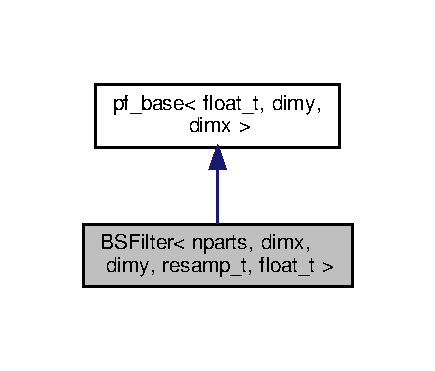
\includegraphics[width=198pt]{classBSFilter__inherit__graph}
\end{center}
\end{figure}


Collaboration diagram for B\+S\+Filter$<$ nparts, dimx, dimy, resamp\+\_\+t, float\+\_\+t, debug $>$\+:\nopagebreak
\begin{figure}[H]
\begin{center}
\leavevmode
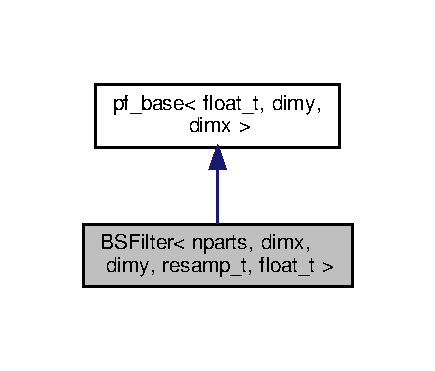
\includegraphics[width=198pt]{classBSFilter__coll__graph}
\end{center}
\end{figure}
\subsection*{Public Types}
\begin{DoxyCompactItemize}
\item 
using \hyperlink{classBSFilter_ad2341b982bcdabc798d7ed0f327d28f7}{ssv} = Eigen\+::\+Matrix$<$ float\+\_\+t, dimx, 1 $>$
\item 
using \hyperlink{classBSFilter_a9a4da560f11a6e2d35ffe693de54826b}{osv} = Eigen\+::\+Matrix$<$ float\+\_\+t, dimy, 1 $>$
\item 
using \hyperlink{classBSFilter_a190a71c131060b131c11ebe2c3fefbeb}{Mat} = Eigen\+::\+Matrix$<$ float\+\_\+t, Eigen\+::\+Dynamic, Eigen\+::\+Dynamic $>$
\item 
using \hyperlink{classBSFilter_a1d6f4a7ba66dda970cd6ea68a70fd641}{array\+States} = std\+::array$<$ \hyperlink{classBSFilter_ad2341b982bcdabc798d7ed0f327d28f7}{ssv}, nparts $>$
\item 
using \hyperlink{classBSFilter_af495dadc972ef1f8d776fe1716177aee}{array\+Float} = std\+::array$<$ float\+\_\+t, nparts $>$
\end{DoxyCompactItemize}
\subsection*{Public Member Functions}
\begin{DoxyCompactItemize}
\item 
\hyperlink{classBSFilter_ab4cab4322cfd2f3f2ed1d4d9b8d058f7}{B\+S\+Filter} (const unsigned int \&rs=1)
\begin{DoxyCompactList}\small\item\em The constructor. \end{DoxyCompactList}\item 
\mbox{\Hypertarget{classBSFilter_a73ee518e89b539464a09430ef541ea7f}\label{classBSFilter_a73ee518e89b539464a09430ef541ea7f}} 
virtual \hyperlink{classBSFilter_a73ee518e89b539464a09430ef541ea7f}{$\sim$\+B\+S\+Filter} ()
\begin{DoxyCompactList}\small\item\em The (virtual) destructor. \end{DoxyCompactList}\item 
float\+\_\+t \hyperlink{classBSFilter_a9cc91baeaaa2a22bff48d82157c86ec5}{get\+Log\+Cond\+Like} () const
\begin{DoxyCompactList}\small\item\em Returns the most recent (log-\/) conditiona likelihood. \end{DoxyCompactList}\item 
void \hyperlink{classBSFilter_a76a59b050d0cc0397b1f594a0a1c22ac}{filter} (const \hyperlink{classBSFilter_a9a4da560f11a6e2d35ffe693de54826b}{osv} \&data, const std\+::vector$<$ std\+::function$<$ const \hyperlink{classBSFilter_a190a71c131060b131c11ebe2c3fefbeb}{Mat}(const \hyperlink{classBSFilter_ad2341b982bcdabc798d7ed0f327d28f7}{ssv} \&)$>$ $>$ \&fs=std\+::vector$<$ std\+::function$<$ const \hyperlink{classBSFilter_a190a71c131060b131c11ebe2c3fefbeb}{Mat}(const \hyperlink{classBSFilter_ad2341b982bcdabc798d7ed0f327d28f7}{ssv} \&)$>$ $>$())
\begin{DoxyCompactList}\small\item\em updates filtering distribution on a new datapoint. Optionally stores expectations of functionals. \end{DoxyCompactList}\item 
auto \hyperlink{classBSFilter_a837a9dc83c07195fb96b4228dc8e41fe}{get\+Expectations} () const -\/$>$ std\+::vector$<$ \hyperlink{classBSFilter_a190a71c131060b131c11ebe2c3fefbeb}{Mat} $>$
\begin{DoxyCompactList}\small\item\em return all stored expectations (taken with respect to \$p(x\+\_\+t$\vert$y\+\_\+\{1\+:t\})\$ \end{DoxyCompactList}\item 
virtual float\+\_\+t \hyperlink{classBSFilter_a460a1a2f97a5d1088a95f6b766e9dc56}{log\+Mu\+Ev} (const \hyperlink{classBSFilter_ad2341b982bcdabc798d7ed0f327d28f7}{ssv} \&x1)=0
\begin{DoxyCompactList}\small\item\em Calculate mu\+Ev or logmu\+Ev. \end{DoxyCompactList}\item 
virtual \hyperlink{classBSFilter_ad2341b982bcdabc798d7ed0f327d28f7}{ssv} \hyperlink{classBSFilter_a82185282cbc7ddf5983933ccd7705577}{q1\+Samp} (const \hyperlink{classBSFilter_a9a4da560f11a6e2d35ffe693de54826b}{osv} \&y1)=0
\begin{DoxyCompactList}\small\item\em Samples from time 1 proposal. \end{DoxyCompactList}\item 
virtual float\+\_\+t \hyperlink{classBSFilter_a81321d8ca9960ea4102c6fe3dc7b7636}{log\+Q1\+Ev} (const \hyperlink{classBSFilter_ad2341b982bcdabc798d7ed0f327d28f7}{ssv} \&x1, const \hyperlink{classBSFilter_a9a4da560f11a6e2d35ffe693de54826b}{osv} \&y1)=0
\begin{DoxyCompactList}\small\item\em Calculate q1\+Ev or log q1\+Ev. \end{DoxyCompactList}\item 
virtual float\+\_\+t \hyperlink{classBSFilter_a1cf2ed5153756a015384d459e72a57de}{log\+G\+Ev} (const \hyperlink{classBSFilter_a9a4da560f11a6e2d35ffe693de54826b}{osv} \&yt, const \hyperlink{classBSFilter_ad2341b982bcdabc798d7ed0f327d28f7}{ssv} \&xt)=0
\begin{DoxyCompactList}\small\item\em Calculate g\+Ev or log\+G\+Ev. \end{DoxyCompactList}\item 
virtual \hyperlink{classBSFilter_ad2341b982bcdabc798d7ed0f327d28f7}{ssv} \hyperlink{classBSFilter_ac97a15ea8002b48e56d94c8de699caa2}{f\+Samp} (const \hyperlink{classBSFilter_ad2341b982bcdabc798d7ed0f327d28f7}{ssv} \&xtm1)=0
\begin{DoxyCompactList}\small\item\em Sample from the state transition distribution. \end{DoxyCompactList}\end{DoxyCompactItemize}
\subsection*{Static Public Attributes}
\begin{DoxyCompactItemize}
\item 
static constexpr unsigned int \hyperlink{classBSFilter_a2a6b1e1870c1a4f3e7ca0b721b697ce2}{num\+\_\+particles} = nparts
\end{DoxyCompactItemize}
\subsection*{Protected Attributes}
\begin{DoxyCompactItemize}
\item 
\mbox{\Hypertarget{classBSFilter_a52dde1eb7fe247f783f4f2e5388f86ac}\label{classBSFilter_a52dde1eb7fe247f783f4f2e5388f86ac}} 
\hyperlink{classBSFilter_a1d6f4a7ba66dda970cd6ea68a70fd641}{array\+States} \hyperlink{classBSFilter_a52dde1eb7fe247f783f4f2e5388f86ac}{m\+\_\+particles}
\begin{DoxyCompactList}\small\item\em particle samples \end{DoxyCompactList}\item 
\mbox{\Hypertarget{classBSFilter_a06b115e9578557bbef4064e43b1afbbe}\label{classBSFilter_a06b115e9578557bbef4064e43b1afbbe}} 
\hyperlink{classBSFilter_af495dadc972ef1f8d776fe1716177aee}{array\+Float} \hyperlink{classBSFilter_a06b115e9578557bbef4064e43b1afbbe}{m\+\_\+log\+Un\+Norm\+Weights}
\begin{DoxyCompactList}\small\item\em particle unnormalized weights \end{DoxyCompactList}\item 
\mbox{\Hypertarget{classBSFilter_adf89ebde89f4ab2d5aa7754042481345}\label{classBSFilter_adf89ebde89f4ab2d5aa7754042481345}} 
unsigned int \hyperlink{classBSFilter_adf89ebde89f4ab2d5aa7754042481345}{m\+\_\+now}
\begin{DoxyCompactList}\small\item\em time point \end{DoxyCompactList}\item 
\mbox{\Hypertarget{classBSFilter_a4aca072edced8670e55023a47ffd551a}\label{classBSFilter_a4aca072edced8670e55023a47ffd551a}} 
float\+\_\+t \hyperlink{classBSFilter_a4aca072edced8670e55023a47ffd551a}{m\+\_\+log\+Last\+Cond\+Like}
\begin{DoxyCompactList}\small\item\em log p(y\+\_\+t$\vert$y\+\_\+\{1\+:t-\/1\}) or log p(y1) \end{DoxyCompactList}\item 
\mbox{\Hypertarget{classBSFilter_aff77ccb7698f098b7d88781a20cef538}\label{classBSFilter_aff77ccb7698f098b7d88781a20cef538}} 
resamp\+\_\+t \hyperlink{classBSFilter_aff77ccb7698f098b7d88781a20cef538}{m\+\_\+resampler}
\begin{DoxyCompactList}\small\item\em resampler object \end{DoxyCompactList}\item 
\mbox{\Hypertarget{classBSFilter_ad36944944fce5d23663245c8cc0a296a}\label{classBSFilter_ad36944944fce5d23663245c8cc0a296a}} 
std\+::vector$<$ \hyperlink{classBSFilter_a190a71c131060b131c11ebe2c3fefbeb}{Mat} $>$ \hyperlink{classBSFilter_ad36944944fce5d23663245c8cc0a296a}{m\+\_\+expectations}
\begin{DoxyCompactList}\small\item\em expectations E\mbox{[}h(x\+\_\+t) $\vert$ y\+\_\+\{1\+:t\}\mbox{]} for user defined \char`\"{}h\char`\"{}s \end{DoxyCompactList}\item 
\mbox{\Hypertarget{classBSFilter_a1962760bd541b6dbea7da7c5572f60e0}\label{classBSFilter_a1962760bd541b6dbea7da7c5572f60e0}} 
unsigned int \hyperlink{classBSFilter_a1962760bd541b6dbea7da7c5572f60e0}{m\+\_\+resamp\+Sched}
\begin{DoxyCompactList}\small\item\em resampling schedule (e.\+g. resample every \+\_\+\+\_\+ time points) \end{DoxyCompactList}\end{DoxyCompactItemize}


\subsection{Detailed Description}
\subsubsection*{template$<$size\+\_\+t nparts, size\+\_\+t dimx, size\+\_\+t dimy, typename resamp\+\_\+t, typename float\+\_\+t, bool debug = false$>$\newline
class B\+S\+Filter$<$ nparts, dimx, dimy, resamp\+\_\+t, float\+\_\+t, debug $>$}

A base class for the bootstrap particle filter. 

\begin{DoxyAuthor}{Author}
taylor 
\end{DoxyAuthor}


\subsection{Member Typedef Documentation}
\mbox{\Hypertarget{classBSFilter_af495dadc972ef1f8d776fe1716177aee}\label{classBSFilter_af495dadc972ef1f8d776fe1716177aee}} 
\index{B\+S\+Filter@{B\+S\+Filter}!array\+Float@{array\+Float}}
\index{array\+Float@{array\+Float}!B\+S\+Filter@{B\+S\+Filter}}
\subsubsection{\texorpdfstring{array\+Float}{arrayFloat}}
{\footnotesize\ttfamily template$<$size\+\_\+t nparts, size\+\_\+t dimx, size\+\_\+t dimy, typename resamp\+\_\+t , typename float\+\_\+t , bool debug = false$>$ \\
using \hyperlink{classBSFilter}{B\+S\+Filter}$<$ nparts, dimx, dimy, resamp\+\_\+t, float\+\_\+t, debug $>$\+::\hyperlink{classBSFilter_af495dadc972ef1f8d776fe1716177aee}{array\+Float} =  std\+::array$<$float\+\_\+t, nparts$>$}

type alias for array of floating points \mbox{\Hypertarget{classBSFilter_a1d6f4a7ba66dda970cd6ea68a70fd641}\label{classBSFilter_a1d6f4a7ba66dda970cd6ea68a70fd641}} 
\index{B\+S\+Filter@{B\+S\+Filter}!array\+States@{array\+States}}
\index{array\+States@{array\+States}!B\+S\+Filter@{B\+S\+Filter}}
\subsubsection{\texorpdfstring{array\+States}{arrayStates}}
{\footnotesize\ttfamily template$<$size\+\_\+t nparts, size\+\_\+t dimx, size\+\_\+t dimy, typename resamp\+\_\+t , typename float\+\_\+t , bool debug = false$>$ \\
using \hyperlink{classBSFilter}{B\+S\+Filter}$<$ nparts, dimx, dimy, resamp\+\_\+t, float\+\_\+t, debug $>$\+::\hyperlink{classBSFilter_a1d6f4a7ba66dda970cd6ea68a70fd641}{array\+States} =  std\+::array$<$\hyperlink{classBSFilter_ad2341b982bcdabc798d7ed0f327d28f7}{ssv}, nparts$>$}

type alias for linear algebra stuff \mbox{\Hypertarget{classBSFilter_a190a71c131060b131c11ebe2c3fefbeb}\label{classBSFilter_a190a71c131060b131c11ebe2c3fefbeb}} 
\index{B\+S\+Filter@{B\+S\+Filter}!Mat@{Mat}}
\index{Mat@{Mat}!B\+S\+Filter@{B\+S\+Filter}}
\subsubsection{\texorpdfstring{Mat}{Mat}}
{\footnotesize\ttfamily template$<$size\+\_\+t nparts, size\+\_\+t dimx, size\+\_\+t dimy, typename resamp\+\_\+t , typename float\+\_\+t , bool debug = false$>$ \\
using \hyperlink{classBSFilter}{B\+S\+Filter}$<$ nparts, dimx, dimy, resamp\+\_\+t, float\+\_\+t, debug $>$\+::\hyperlink{classBSFilter_a190a71c131060b131c11ebe2c3fefbeb}{Mat} =  Eigen\+::\+Matrix$<$float\+\_\+t, Eigen\+::\+Dynamic, Eigen\+::\+Dynamic$>$}

type alias for dynamically sized matrix \mbox{\Hypertarget{classBSFilter_a9a4da560f11a6e2d35ffe693de54826b}\label{classBSFilter_a9a4da560f11a6e2d35ffe693de54826b}} 
\index{B\+S\+Filter@{B\+S\+Filter}!osv@{osv}}
\index{osv@{osv}!B\+S\+Filter@{B\+S\+Filter}}
\subsubsection{\texorpdfstring{osv}{osv}}
{\footnotesize\ttfamily template$<$size\+\_\+t nparts, size\+\_\+t dimx, size\+\_\+t dimy, typename resamp\+\_\+t , typename float\+\_\+t , bool debug = false$>$ \\
using \hyperlink{classBSFilter}{B\+S\+Filter}$<$ nparts, dimx, dimy, resamp\+\_\+t, float\+\_\+t, debug $>$\+::\hyperlink{classBSFilter_a9a4da560f11a6e2d35ffe693de54826b}{osv} =  Eigen\+::\+Matrix$<$float\+\_\+t, dimy, 1$>$}

\char`\"{}obs size vector\char`\"{} type alias for linear algebra stuff \mbox{\Hypertarget{classBSFilter_ad2341b982bcdabc798d7ed0f327d28f7}\label{classBSFilter_ad2341b982bcdabc798d7ed0f327d28f7}} 
\index{B\+S\+Filter@{B\+S\+Filter}!ssv@{ssv}}
\index{ssv@{ssv}!B\+S\+Filter@{B\+S\+Filter}}
\subsubsection{\texorpdfstring{ssv}{ssv}}
{\footnotesize\ttfamily template$<$size\+\_\+t nparts, size\+\_\+t dimx, size\+\_\+t dimy, typename resamp\+\_\+t , typename float\+\_\+t , bool debug = false$>$ \\
using \hyperlink{classBSFilter}{B\+S\+Filter}$<$ nparts, dimx, dimy, resamp\+\_\+t, float\+\_\+t, debug $>$\+::\hyperlink{classBSFilter_ad2341b982bcdabc798d7ed0f327d28f7}{ssv} =  Eigen\+::\+Matrix$<$float\+\_\+t, dimx, 1$>$}

\char`\"{}state size vector\char`\"{} type alias for linear algebra stuff 

\subsection{Constructor \& Destructor Documentation}
\mbox{\Hypertarget{classBSFilter_ab4cab4322cfd2f3f2ed1d4d9b8d058f7}\label{classBSFilter_ab4cab4322cfd2f3f2ed1d4d9b8d058f7}} 
\index{B\+S\+Filter@{B\+S\+Filter}!B\+S\+Filter@{B\+S\+Filter}}
\index{B\+S\+Filter@{B\+S\+Filter}!B\+S\+Filter@{B\+S\+Filter}}
\subsubsection{\texorpdfstring{B\+S\+Filter()}{BSFilter()}}
{\footnotesize\ttfamily template$<$size\+\_\+t nparts, size\+\_\+t dimx, size\+\_\+t dimy, typename resamp\+\_\+t , typename float\+\_\+t , bool debug$>$ \\
\hyperlink{classBSFilter}{B\+S\+Filter}$<$ nparts, dimx, dimy, resamp\+\_\+t, float\+\_\+t, debug $>$\+::\hyperlink{classBSFilter}{B\+S\+Filter} (\begin{DoxyParamCaption}\item[{const unsigned int \&}]{rs = {\ttfamily 1} }\end{DoxyParamCaption})}



The constructor. 


\begin{DoxyParams}{Parameters}
{\em rs} & the resampling schedule (e.\+g. every rs time point) \\
\hline
\end{DoxyParams}


\subsection{Member Function Documentation}
\mbox{\Hypertarget{classBSFilter_a76a59b050d0cc0397b1f594a0a1c22ac}\label{classBSFilter_a76a59b050d0cc0397b1f594a0a1c22ac}} 
\index{B\+S\+Filter@{B\+S\+Filter}!filter@{filter}}
\index{filter@{filter}!B\+S\+Filter@{B\+S\+Filter}}
\subsubsection{\texorpdfstring{filter()}{filter()}}
{\footnotesize\ttfamily template$<$size\+\_\+t nparts, size\+\_\+t dimx, size\+\_\+t dimy, typename resamp\+\_\+t , typename float\+\_\+t , bool debug$>$ \\
void \hyperlink{classBSFilter}{B\+S\+Filter}$<$ nparts, dimx, dimy, resamp\+\_\+t, float\+\_\+t, debug $>$\+::filter (\begin{DoxyParamCaption}\item[{const \hyperlink{classBSFilter_a9a4da560f11a6e2d35ffe693de54826b}{osv} \&}]{data,  }\item[{const std\+::vector$<$ std\+::function$<$ const \hyperlink{classBSFilter_a190a71c131060b131c11ebe2c3fefbeb}{Mat}(const \hyperlink{classBSFilter_ad2341b982bcdabc798d7ed0f327d28f7}{ssv} \&)$>$ $>$ \&}]{fs = {\ttfamily std\+:\+:vector$<$std\+:\+:function$<$const~\hyperlink{classBSFilter_a190a71c131060b131c11ebe2c3fefbeb}{Mat}(const~\hyperlink{classBSFilter_ad2341b982bcdabc798d7ed0f327d28f7}{ssv}\&)$>$~$>$()} }\end{DoxyParamCaption})}



updates filtering distribution on a new datapoint. Optionally stores expectations of functionals. 


\begin{DoxyParams}{Parameters}
{\em data} & the most recent data point \\
\hline
{\em fs} & a vector of functions if you want to calculate expectations. \\
\hline
\end{DoxyParams}
\mbox{\Hypertarget{classBSFilter_ac97a15ea8002b48e56d94c8de699caa2}\label{classBSFilter_ac97a15ea8002b48e56d94c8de699caa2}} 
\index{B\+S\+Filter@{B\+S\+Filter}!f\+Samp@{f\+Samp}}
\index{f\+Samp@{f\+Samp}!B\+S\+Filter@{B\+S\+Filter}}
\subsubsection{\texorpdfstring{f\+Samp()}{fSamp()}}
{\footnotesize\ttfamily template$<$size\+\_\+t nparts, size\+\_\+t dimx, size\+\_\+t dimy, typename resamp\+\_\+t , typename float\+\_\+t , bool debug = false$>$ \\
virtual \hyperlink{classBSFilter_ad2341b982bcdabc798d7ed0f327d28f7}{ssv} \hyperlink{classBSFilter}{B\+S\+Filter}$<$ nparts, dimx, dimy, resamp\+\_\+t, float\+\_\+t, debug $>$\+::f\+Samp (\begin{DoxyParamCaption}\item[{const \hyperlink{classBSFilter_ad2341b982bcdabc798d7ed0f327d28f7}{ssv} \&}]{xtm1 }\end{DoxyParamCaption})\hspace{0.3cm}{\ttfamily [pure virtual]}}



Sample from the state transition distribution. 


\begin{DoxyParams}{Parameters}
{\em xtm1} & is a const Vec\& describing the time t-\/1 state \\
\hline
\end{DoxyParams}
\begin{DoxyReturn}{Returns}
the sample as a Vec 
\end{DoxyReturn}
\mbox{\Hypertarget{classBSFilter_a837a9dc83c07195fb96b4228dc8e41fe}\label{classBSFilter_a837a9dc83c07195fb96b4228dc8e41fe}} 
\index{B\+S\+Filter@{B\+S\+Filter}!get\+Expectations@{get\+Expectations}}
\index{get\+Expectations@{get\+Expectations}!B\+S\+Filter@{B\+S\+Filter}}
\subsubsection{\texorpdfstring{get\+Expectations()}{getExpectations()}}
{\footnotesize\ttfamily template$<$size\+\_\+t nparts, size\+\_\+t dimx, size\+\_\+t dimy, typename resamp\+\_\+t , typename float\+\_\+t , bool debug$>$ \\
auto \hyperlink{classBSFilter}{B\+S\+Filter}$<$ nparts, dimx, dimy, resamp\+\_\+t, float\+\_\+t, debug $>$\+::get\+Expectations (\begin{DoxyParamCaption}{ }\end{DoxyParamCaption}) const -\/$>$ std\+::vector$<$\hyperlink{classBSFilter_a190a71c131060b131c11ebe2c3fefbeb}{Mat}$>$}



return all stored expectations (taken with respect to \$p(x\+\_\+t$\vert$y\+\_\+\{1\+:t\})\$ 

\begin{DoxyReturn}{Returns}
return a std\+::vector$<$\+Mat$>$ of expectations. How many depends on how many callbacks you gave to 
\end{DoxyReturn}
\mbox{\Hypertarget{classBSFilter_a9cc91baeaaa2a22bff48d82157c86ec5}\label{classBSFilter_a9cc91baeaaa2a22bff48d82157c86ec5}} 
\index{B\+S\+Filter@{B\+S\+Filter}!get\+Log\+Cond\+Like@{get\+Log\+Cond\+Like}}
\index{get\+Log\+Cond\+Like@{get\+Log\+Cond\+Like}!B\+S\+Filter@{B\+S\+Filter}}
\subsubsection{\texorpdfstring{get\+Log\+Cond\+Like()}{getLogCondLike()}}
{\footnotesize\ttfamily template$<$size\+\_\+t nparts, size\+\_\+t dimx, size\+\_\+t dimy, typename resamp\+\_\+t , typename float\+\_\+t , bool debug$>$ \\
float\+\_\+t \hyperlink{classBSFilter}{B\+S\+Filter}$<$ nparts, dimx, dimy, resamp\+\_\+t, float\+\_\+t, debug $>$\+::get\+Log\+Cond\+Like (\begin{DoxyParamCaption}{ }\end{DoxyParamCaption}) const\hspace{0.3cm}{\ttfamily [virtual]}}



Returns the most recent (log-\/) conditiona likelihood. 

\begin{DoxyReturn}{Returns}
log p(y\+\_\+t $\vert$ y\+\_\+\{1\+:t-\/1\}) 
\end{DoxyReturn}


Implements \hyperlink{classpf__base_a350df818820d6ab0fd6d413022b7f23b}{pf\+\_\+base$<$ float\+\_\+t, dimy, dimx $>$}.

\mbox{\Hypertarget{classBSFilter_a1cf2ed5153756a015384d459e72a57de}\label{classBSFilter_a1cf2ed5153756a015384d459e72a57de}} 
\index{B\+S\+Filter@{B\+S\+Filter}!log\+G\+Ev@{log\+G\+Ev}}
\index{log\+G\+Ev@{log\+G\+Ev}!B\+S\+Filter@{B\+S\+Filter}}
\subsubsection{\texorpdfstring{log\+G\+Ev()}{logGEv()}}
{\footnotesize\ttfamily template$<$size\+\_\+t nparts, size\+\_\+t dimx, size\+\_\+t dimy, typename resamp\+\_\+t , typename float\+\_\+t , bool debug = false$>$ \\
virtual float\+\_\+t \hyperlink{classBSFilter}{B\+S\+Filter}$<$ nparts, dimx, dimy, resamp\+\_\+t, float\+\_\+t, debug $>$\+::log\+G\+Ev (\begin{DoxyParamCaption}\item[{const \hyperlink{classBSFilter_a9a4da560f11a6e2d35ffe693de54826b}{osv} \&}]{yt,  }\item[{const \hyperlink{classBSFilter_ad2341b982bcdabc798d7ed0f327d28f7}{ssv} \&}]{xt }\end{DoxyParamCaption})\hspace{0.3cm}{\ttfamily [pure virtual]}}



Calculate g\+Ev or log\+G\+Ev. 


\begin{DoxyParams}{Parameters}
{\em yt} & is a const Vec\& describing the time t datum \\
\hline
{\em xt} & is a const Vec\& describing the time t state \\
\hline
\end{DoxyParams}
\begin{DoxyReturn}{Returns}
the density or log-\/density evaluation 
\end{DoxyReturn}
\mbox{\Hypertarget{classBSFilter_a460a1a2f97a5d1088a95f6b766e9dc56}\label{classBSFilter_a460a1a2f97a5d1088a95f6b766e9dc56}} 
\index{B\+S\+Filter@{B\+S\+Filter}!log\+Mu\+Ev@{log\+Mu\+Ev}}
\index{log\+Mu\+Ev@{log\+Mu\+Ev}!B\+S\+Filter@{B\+S\+Filter}}
\subsubsection{\texorpdfstring{log\+Mu\+Ev()}{logMuEv()}}
{\footnotesize\ttfamily template$<$size\+\_\+t nparts, size\+\_\+t dimx, size\+\_\+t dimy, typename resamp\+\_\+t , typename float\+\_\+t , bool debug = false$>$ \\
virtual float\+\_\+t \hyperlink{classBSFilter}{B\+S\+Filter}$<$ nparts, dimx, dimy, resamp\+\_\+t, float\+\_\+t, debug $>$\+::log\+Mu\+Ev (\begin{DoxyParamCaption}\item[{const \hyperlink{classBSFilter_ad2341b982bcdabc798d7ed0f327d28f7}{ssv} \&}]{x1 }\end{DoxyParamCaption})\hspace{0.3cm}{\ttfamily [pure virtual]}}



Calculate mu\+Ev or logmu\+Ev. 


\begin{DoxyParams}{Parameters}
{\em x1} & is a const Vec\& describing the state sample \\
\hline
\end{DoxyParams}
\begin{DoxyReturn}{Returns}
the density or log-\/density evaluation 
\end{DoxyReturn}
\mbox{\Hypertarget{classBSFilter_a81321d8ca9960ea4102c6fe3dc7b7636}\label{classBSFilter_a81321d8ca9960ea4102c6fe3dc7b7636}} 
\index{B\+S\+Filter@{B\+S\+Filter}!log\+Q1\+Ev@{log\+Q1\+Ev}}
\index{log\+Q1\+Ev@{log\+Q1\+Ev}!B\+S\+Filter@{B\+S\+Filter}}
\subsubsection{\texorpdfstring{log\+Q1\+Ev()}{logQ1Ev()}}
{\footnotesize\ttfamily template$<$size\+\_\+t nparts, size\+\_\+t dimx, size\+\_\+t dimy, typename resamp\+\_\+t , typename float\+\_\+t , bool debug = false$>$ \\
virtual float\+\_\+t \hyperlink{classBSFilter}{B\+S\+Filter}$<$ nparts, dimx, dimy, resamp\+\_\+t, float\+\_\+t, debug $>$\+::log\+Q1\+Ev (\begin{DoxyParamCaption}\item[{const \hyperlink{classBSFilter_ad2341b982bcdabc798d7ed0f327d28f7}{ssv} \&}]{x1,  }\item[{const \hyperlink{classBSFilter_a9a4da560f11a6e2d35ffe693de54826b}{osv} \&}]{y1 }\end{DoxyParamCaption})\hspace{0.3cm}{\ttfamily [pure virtual]}}



Calculate q1\+Ev or log q1\+Ev. 


\begin{DoxyParams}{Parameters}
{\em x1} & is a const Vec\& describing the time 1 state sample \\
\hline
{\em y1} & is a const Vec\& describing the time 1 datum \\
\hline
\end{DoxyParams}
\begin{DoxyReturn}{Returns}
the density or log-\/density evaluation 
\end{DoxyReturn}
\mbox{\Hypertarget{classBSFilter_a82185282cbc7ddf5983933ccd7705577}\label{classBSFilter_a82185282cbc7ddf5983933ccd7705577}} 
\index{B\+S\+Filter@{B\+S\+Filter}!q1\+Samp@{q1\+Samp}}
\index{q1\+Samp@{q1\+Samp}!B\+S\+Filter@{B\+S\+Filter}}
\subsubsection{\texorpdfstring{q1\+Samp()}{q1Samp()}}
{\footnotesize\ttfamily template$<$size\+\_\+t nparts, size\+\_\+t dimx, size\+\_\+t dimy, typename resamp\+\_\+t , typename float\+\_\+t , bool debug = false$>$ \\
virtual \hyperlink{classBSFilter_ad2341b982bcdabc798d7ed0f327d28f7}{ssv} \hyperlink{classBSFilter}{B\+S\+Filter}$<$ nparts, dimx, dimy, resamp\+\_\+t, float\+\_\+t, debug $>$\+::q1\+Samp (\begin{DoxyParamCaption}\item[{const \hyperlink{classBSFilter_a9a4da560f11a6e2d35ffe693de54826b}{osv} \&}]{y1 }\end{DoxyParamCaption})\hspace{0.3cm}{\ttfamily [pure virtual]}}



Samples from time 1 proposal. 


\begin{DoxyParams}{Parameters}
{\em y1} & is a const Vec\& representing the first observed datum \\
\hline
\end{DoxyParams}
\begin{DoxyReturn}{Returns}
the sample as a Vec 
\end{DoxyReturn}


\subsection{Member Data Documentation}
\mbox{\Hypertarget{classBSFilter_a2a6b1e1870c1a4f3e7ca0b721b697ce2}\label{classBSFilter_a2a6b1e1870c1a4f3e7ca0b721b697ce2}} 
\index{B\+S\+Filter@{B\+S\+Filter}!num\+\_\+particles@{num\+\_\+particles}}
\index{num\+\_\+particles@{num\+\_\+particles}!B\+S\+Filter@{B\+S\+Filter}}
\subsubsection{\texorpdfstring{num\+\_\+particles}{num\_particles}}
{\footnotesize\ttfamily template$<$size\+\_\+t nparts, size\+\_\+t dimx, size\+\_\+t dimy, typename resamp\+\_\+t , typename float\+\_\+t , bool debug = false$>$ \\
constexpr unsigned int \hyperlink{classBSFilter}{B\+S\+Filter}$<$ nparts, dimx, dimy, resamp\+\_\+t, float\+\_\+t, debug $>$\+::num\+\_\+particles = nparts\hspace{0.3cm}{\ttfamily [static]}}

the number of particles 

The documentation for this class was generated from the following file\+:\begin{DoxyCompactItemize}
\item 
include/pf/\hyperlink{bootstrap__filter_8h}{bootstrap\+\_\+filter.\+h}\end{DoxyCompactItemize}

\hypertarget{classk__gen}{}\section{k\+\_\+gen$<$ N $>$ Class Template Reference}
\label{classk__gen}\index{k\+\_\+gen$<$ N $>$@{k\+\_\+gen$<$ N $>$}}


A class that performs sampling with replacement (useful for the index sampler in an \hyperlink{classAPF}{A\+PF})  




{\ttfamily \#include $<$rv\+\_\+samp.\+h$>$}



Inheritance diagram for k\+\_\+gen$<$ N $>$\+:\nopagebreak
\begin{figure}[H]
\begin{center}
\leavevmode
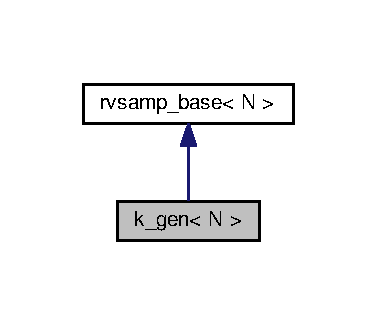
\includegraphics[width=181pt]{classk__gen__inherit__graph}
\end{center}
\end{figure}


Collaboration diagram for k\+\_\+gen$<$ N $>$\+:\nopagebreak
\begin{figure}[H]
\begin{center}
\leavevmode
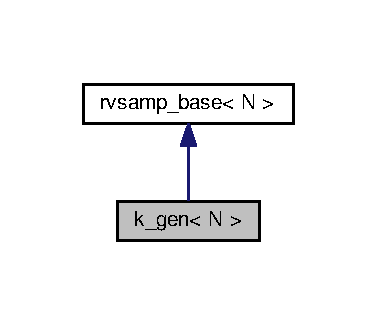
\includegraphics[width=181pt]{classk__gen__coll__graph}
\end{center}
\end{figure}
\subsection*{Public Member Functions}
\begin{DoxyCompactItemize}
\item 
\hyperlink{classk__gen_ace54048feceb6965d7c3b51c5a4b7eea}{k\+\_\+gen} ()\hypertarget{classk__gen_ace54048feceb6965d7c3b51c5a4b7eea}{}\label{classk__gen_ace54048feceb6965d7c3b51c5a4b7eea}

\begin{DoxyCompactList}\small\item\em default constructor. only one available. \end{DoxyCompactList}\item 
std\+::array$<$ unsigned int, N $>$ \hyperlink{classk__gen_a9256cf954970f71dc1c5ce36081b2364}{sample} (const std\+::array$<$ double, N $>$ \&log\+Wts)
\begin{DoxyCompactList}\small\item\em sample N times from (0,1,...N-\/1) \end{DoxyCompactList}\end{DoxyCompactItemize}
\subsection*{Additional Inherited Members}


\subsection{Detailed Description}
\subsubsection*{template$<$size\+\_\+t N$>$\\*
class k\+\_\+gen$<$ N $>$}

A class that performs sampling with replacement (useful for the index sampler in an \hyperlink{classAPF}{A\+PF}) 

\begin{DoxyAuthor}{Author}
taylor 
\end{DoxyAuthor}


\subsection{Member Function Documentation}
\index{k\+\_\+gen@{k\+\_\+gen}!sample@{sample}}
\index{sample@{sample}!k\+\_\+gen@{k\+\_\+gen}}
\subsubsection[{\texorpdfstring{sample(const std\+::array$<$ double, N $>$ \&log\+Wts)}{sample(const std::array< double, N > &logWts)}}]{\setlength{\rightskip}{0pt plus 5cm}template$<$size\+\_\+t N$>$ std\+::array$<$ unsigned int, N $>$ {\bf k\+\_\+gen}$<$ N $>$\+::sample (
\begin{DoxyParamCaption}
\item[{const std\+::array$<$ double, N $>$ \&}]{log\+Wts}
\end{DoxyParamCaption}
)}\hypertarget{classk__gen_a9256cf954970f71dc1c5ce36081b2364}{}\label{classk__gen_a9256cf954970f71dc1c5ce36081b2364}


sample N times from (0,1,...N-\/1) 


\begin{DoxyParams}{Parameters}
{\em log\+Wts} & possibly unnormalized type std\+::array$<$double, N$>$ \\
\hline
\end{DoxyParams}
\begin{DoxyReturn}{Returns}
the integers in a std\+::array$<$unsigned int, N$>$ 
\end{DoxyReturn}


The documentation for this class was generated from the following file\+:\begin{DoxyCompactItemize}
\item 
include/\hyperlink{rv__samp_8h}{rv\+\_\+samp.\+h}\end{DoxyCompactItemize}

\hypertarget{classmn__resampler}{}\section{mn\+\_\+resampler$<$ nparts, dimx, float\+\_\+t $>$ Class Template Reference}
\label{classmn__resampler}\index{mn\+\_\+resampler$<$ nparts, dimx, float\+\_\+t $>$@{mn\+\_\+resampler$<$ nparts, dimx, float\+\_\+t $>$}}


{\ttfamily \#include $<$resamplers.\+h$>$}



Inheritance diagram for mn\+\_\+resampler$<$ nparts, dimx, float\+\_\+t $>$\+:\nopagebreak
\begin{figure}[H]
\begin{center}
\leavevmode
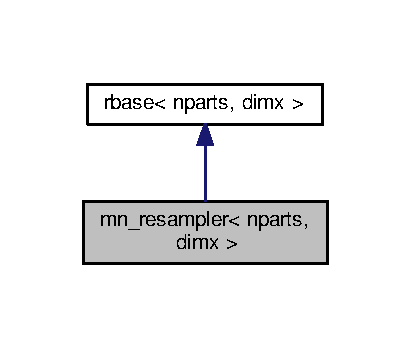
\includegraphics[width=197pt]{classmn__resampler__inherit__graph}
\end{center}
\end{figure}


Collaboration diagram for mn\+\_\+resampler$<$ nparts, dimx, float\+\_\+t $>$\+:\nopagebreak
\begin{figure}[H]
\begin{center}
\leavevmode
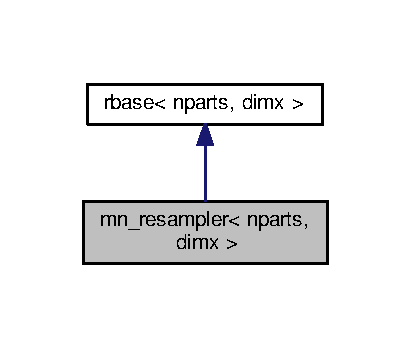
\includegraphics[width=197pt]{classmn__resampler__coll__graph}
\end{center}
\end{figure}
\subsection*{Public Types}
\begin{DoxyCompactItemize}
\item 
using \hyperlink{classmn__resampler_a1cb075b42f73e01de7fc1b27f51bfc4c}{ssv} = Eigen\+::\+Matrix$<$ float\+\_\+t, dimx, 1 $>$
\item 
using \hyperlink{classmn__resampler_aa8ff37576399807b14a7a12615032bb1}{array\+Vec} = std\+::array$<$ \hyperlink{classrbase_ae20e0b8df15aa109252f57ecbf1f20f8}{ssv}, nparts $>$
\item 
using \hyperlink{classmn__resampler_ae26be2889cf3cd4ddea66928d879809e}{array\+Float} = std\+::array$<$ float\+\_\+t, nparts $>$
\item 
using \hyperlink{classmn__resampler_afb5d000e2464afef813792c57c42599b}{array\+Int} = std\+::array$<$ unsigned int, nparts $>$
\end{DoxyCompactItemize}
\subsection*{Public Member Functions}
\begin{DoxyCompactItemize}
\item 
\mbox{\Hypertarget{classmn__resampler_a016a00570c30806a0fdad25385395f95}\label{classmn__resampler_a016a00570c30806a0fdad25385395f95}} 
\hyperlink{classmn__resampler_a016a00570c30806a0fdad25385395f95}{mn\+\_\+resampler} ()=default
\begin{DoxyCompactList}\small\item\em Default constructor. Only option available. \end{DoxyCompactList}\item 
void \hyperlink{classmn__resampler_a13b1897e180a791a3a099d5d6329a125}{resamp\+Log\+Wts} (\hyperlink{classrbase_aa12fc826befa6ba0647b5f59ebc396ee}{array\+Vec} \&old\+Parts, \hyperlink{classrbase_a6f76bef853e508cb5b6f546d231b06f5}{array\+Float} \&old\+Log\+Un\+Norm\+Wts)
\begin{DoxyCompactList}\small\item\em resamples particles. \end{DoxyCompactList}\end{DoxyCompactItemize}
\subsection*{Additional Inherited Members}


\subsection{Detailed Description}
\subsubsection*{template$<$size\+\_\+t nparts, size\+\_\+t dimx, typename float\+\_\+t$>$\newline
class mn\+\_\+resampler$<$ nparts, dimx, float\+\_\+t $>$}

\begin{DoxyAuthor}{Author}
taylor 
\end{DoxyAuthor}
\begin{DoxyDate}{Date}
15/04/18 
\end{DoxyDate}


\subsection{Member Typedef Documentation}
\mbox{\Hypertarget{classmn__resampler_ae26be2889cf3cd4ddea66928d879809e}\label{classmn__resampler_ae26be2889cf3cd4ddea66928d879809e}} 
\index{mn\+\_\+resampler@{mn\+\_\+resampler}!array\+Float@{array\+Float}}
\index{array\+Float@{array\+Float}!mn\+\_\+resampler@{mn\+\_\+resampler}}
\subsubsection{\texorpdfstring{array\+Float}{arrayFloat}}
{\footnotesize\ttfamily template$<$size\+\_\+t nparts, size\+\_\+t dimx, typename float\+\_\+t $>$ \\
using \hyperlink{classmn__resampler}{mn\+\_\+resampler}$<$ nparts, dimx, float\+\_\+t $>$\+::\hyperlink{classrbase_a6f76bef853e508cb5b6f546d231b06f5}{array\+Float} =  std\+::array$<$float\+\_\+t,nparts$>$}

type alias for array of float\+\_\+ts \mbox{\Hypertarget{classmn__resampler_afb5d000e2464afef813792c57c42599b}\label{classmn__resampler_afb5d000e2464afef813792c57c42599b}} 
\index{mn\+\_\+resampler@{mn\+\_\+resampler}!array\+Int@{array\+Int}}
\index{array\+Int@{array\+Int}!mn\+\_\+resampler@{mn\+\_\+resampler}}
\subsubsection{\texorpdfstring{array\+Int}{arrayInt}}
{\footnotesize\ttfamily template$<$size\+\_\+t nparts, size\+\_\+t dimx, typename float\+\_\+t $>$ \\
using \hyperlink{classmn__resampler}{mn\+\_\+resampler}$<$ nparts, dimx, float\+\_\+t $>$\+::\hyperlink{classmn__resampler_afb5d000e2464afef813792c57c42599b}{array\+Int} =  std\+::array$<$unsigned int,nparts$>$}

type alias for array of integers \mbox{\Hypertarget{classmn__resampler_aa8ff37576399807b14a7a12615032bb1}\label{classmn__resampler_aa8ff37576399807b14a7a12615032bb1}} 
\index{mn\+\_\+resampler@{mn\+\_\+resampler}!array\+Vec@{array\+Vec}}
\index{array\+Vec@{array\+Vec}!mn\+\_\+resampler@{mn\+\_\+resampler}}
\subsubsection{\texorpdfstring{array\+Vec}{arrayVec}}
{\footnotesize\ttfamily template$<$size\+\_\+t nparts, size\+\_\+t dimx, typename float\+\_\+t $>$ \\
using \hyperlink{classmn__resampler}{mn\+\_\+resampler}$<$ nparts, dimx, float\+\_\+t $>$\+::\hyperlink{classrbase_aa12fc826befa6ba0647b5f59ebc396ee}{array\+Vec} =  std\+::array$<$\hyperlink{classrbase_ae20e0b8df15aa109252f57ecbf1f20f8}{ssv}, nparts$>$}

type alias for array of Eigen Matrices \mbox{\Hypertarget{classmn__resampler_a1cb075b42f73e01de7fc1b27f51bfc4c}\label{classmn__resampler_a1cb075b42f73e01de7fc1b27f51bfc4c}} 
\index{mn\+\_\+resampler@{mn\+\_\+resampler}!ssv@{ssv}}
\index{ssv@{ssv}!mn\+\_\+resampler@{mn\+\_\+resampler}}
\subsubsection{\texorpdfstring{ssv}{ssv}}
{\footnotesize\ttfamily template$<$size\+\_\+t nparts, size\+\_\+t dimx, typename float\+\_\+t $>$ \\
using \hyperlink{classmn__resampler}{mn\+\_\+resampler}$<$ nparts, dimx, float\+\_\+t $>$\+::\hyperlink{classrbase_ae20e0b8df15aa109252f57ecbf1f20f8}{ssv} =  Eigen\+::\+Matrix$<$float\+\_\+t,dimx,1$>$}

type alias for linear algebra stuff 

\subsection{Member Function Documentation}
\mbox{\Hypertarget{classmn__resampler_a13b1897e180a791a3a099d5d6329a125}\label{classmn__resampler_a13b1897e180a791a3a099d5d6329a125}} 
\index{mn\+\_\+resampler@{mn\+\_\+resampler}!resamp\+Log\+Wts@{resamp\+Log\+Wts}}
\index{resamp\+Log\+Wts@{resamp\+Log\+Wts}!mn\+\_\+resampler@{mn\+\_\+resampler}}
\subsubsection{\texorpdfstring{resamp\+Log\+Wts()}{resampLogWts()}}
{\footnotesize\ttfamily template$<$size\+\_\+t nparts, size\+\_\+t dimx, typename float\+\_\+t $>$ \\
void \hyperlink{classmn__resampler}{mn\+\_\+resampler}$<$ nparts, dimx, float\+\_\+t $>$\+::resamp\+Log\+Wts (\begin{DoxyParamCaption}\item[{\hyperlink{classrbase_aa12fc826befa6ba0647b5f59ebc396ee}{array\+Vec} \&}]{old\+Parts,  }\item[{\hyperlink{classrbase_a6f76bef853e508cb5b6f546d231b06f5}{array\+Float} \&}]{old\+Log\+Un\+Norm\+Wts }\end{DoxyParamCaption})\hspace{0.3cm}{\ttfamily [virtual]}}



resamples particles. 


\begin{DoxyParams}{Parameters}
{\em old\+Parts} & the old particles \\
\hline
{\em old\+Log\+Un\+Norm\+Wts} & the old log unnormalized weights \\
\hline
\end{DoxyParams}


Implements \hyperlink{classrbase_aff0f6f88fd4656e67f5ebc870f10dd44}{rbase$<$ nparts, dimx, float\+\_\+t $>$}.



The documentation for this class was generated from the following file\+:\begin{DoxyCompactItemize}
\item 
include/pf/\hyperlink{resamplers_8h}{resamplers.\+h}\end{DoxyCompactItemize}

\hypertarget{classMVNSampler}{}\section{M\+V\+N\+Sampler$<$ dim $>$ Class Template Reference}
\label{classMVNSampler}\index{M\+V\+N\+Sampler$<$ dim $>$@{M\+V\+N\+Sampler$<$ dim $>$}}


A class that performs sampling from a multivariate normal distribution.  




{\ttfamily \#include $<$rv\+\_\+samp.\+h$>$}



Inheritance diagram for M\+V\+N\+Sampler$<$ dim $>$\+:\nopagebreak
\begin{figure}[H]
\begin{center}
\leavevmode
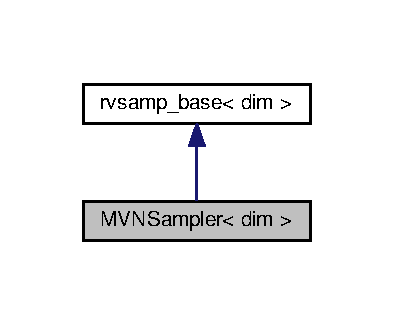
\includegraphics[width=189pt]{classMVNSampler__inherit__graph}
\end{center}
\end{figure}


Collaboration diagram for M\+V\+N\+Sampler$<$ dim $>$\+:\nopagebreak
\begin{figure}[H]
\begin{center}
\leavevmode
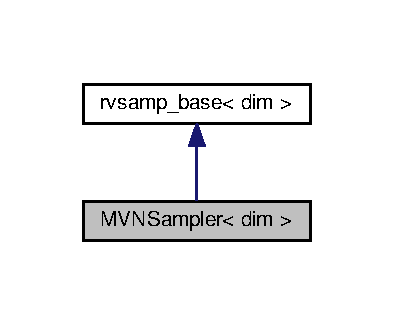
\includegraphics[width=189pt]{classMVNSampler__coll__graph}
\end{center}
\end{figure}
\subsection*{Public Types}
\begin{DoxyCompactItemize}
\item 
using \hyperlink{classMVNSampler_a409f73d7a66202b7ecff0f86e9afe3c1}{Vec} = Eigen\+::\+Matrix$<$ double, dim, 1 $>$
\item 
using \hyperlink{classMVNSampler_a008de968c985ee41633d53d25174701f}{Mat} = Eigen\+::\+Matrix$<$ double, dim, dim $>$
\end{DoxyCompactItemize}
\subsection*{Public Member Functions}
\begin{DoxyCompactItemize}
\item 
\hyperlink{classMVNSampler_a707349ecff1586c9477ffa399f014456}{M\+V\+N\+Sampler} ()
\begin{DoxyCompactList}\small\item\em Default-\/constructor sets up for multivariate standard Normal random variate generation. \end{DoxyCompactList}\item 
\hyperlink{classMVNSampler_a5ff0c96fe23f68ae910c11d6636aacf4}{M\+V\+N\+Sampler} (const \hyperlink{classMVNSampler_a409f73d7a66202b7ecff0f86e9afe3c1}{Vec} \&mean\+Vec, const \hyperlink{classMVNSampler_a008de968c985ee41633d53d25174701f}{Mat} \&cov\+Mat)
\begin{DoxyCompactList}\small\item\em The user must supply both mean and covariance matrix. \end{DoxyCompactList}\item 
void \hyperlink{classMVNSampler_a048a0f48cfb72718faf140e74e9a3ccb}{set\+Covar} (const \hyperlink{classMVNSampler_a008de968c985ee41633d53d25174701f}{Mat} \&cov\+Mat)
\begin{DoxyCompactList}\small\item\em sets the covariance matrix of the sampler. \end{DoxyCompactList}\item 
void \hyperlink{classMVNSampler_a842ee5e6925f50881b6628821a5de717}{set\+Mean} (const \hyperlink{classMVNSampler_a409f73d7a66202b7ecff0f86e9afe3c1}{Vec} \&mean\+Vec)
\begin{DoxyCompactList}\small\item\em sets the mean vector of the sampler. \end{DoxyCompactList}\item 
auto \hyperlink{classMVNSampler_a9c4d69cdbe841255a6fc1ff8531c4f4e}{sample} () -\/$>$ \hyperlink{classMVNSampler_a409f73d7a66202b7ecff0f86e9afe3c1}{Vec}
\begin{DoxyCompactList}\small\item\em Draws a random vector. \end{DoxyCompactList}\end{DoxyCompactItemize}
\subsection*{Private Attributes}
\begin{DoxyCompactItemize}
\item 
std\+::normal\+\_\+distribution \hyperlink{classMVNSampler_a4b68c9586aa0b10f27437aebb370869f}{m\+\_\+z\+\_\+gen}\hypertarget{classMVNSampler_a4b68c9586aa0b10f27437aebb370869f}{}\label{classMVNSampler_a4b68c9586aa0b10f27437aebb370869f}

\begin{DoxyCompactList}\small\item\em makes normal random variates \end{DoxyCompactList}\item 
\hyperlink{classMVNSampler_a008de968c985ee41633d53d25174701f}{Mat} \hyperlink{classMVNSampler_a59c5a532bceb4156205d32d239458696}{m\+\_\+scale\+\_\+mat}\hypertarget{classMVNSampler_a59c5a532bceb4156205d32d239458696}{}\label{classMVNSampler_a59c5a532bceb4156205d32d239458696}

\begin{DoxyCompactList}\small\item\em covariance matrix \end{DoxyCompactList}\item 
\hyperlink{classMVNSampler_a409f73d7a66202b7ecff0f86e9afe3c1}{Vec} \hyperlink{classMVNSampler_abe79aa245de63b44eb25c1fa56cffb73}{m\+\_\+mean}\hypertarget{classMVNSampler_abe79aa245de63b44eb25c1fa56cffb73}{}\label{classMVNSampler_abe79aa245de63b44eb25c1fa56cffb73}

\begin{DoxyCompactList}\small\item\em mean vector \end{DoxyCompactList}\end{DoxyCompactItemize}
\subsection*{Additional Inherited Members}


\subsection{Detailed Description}
\subsubsection*{template$<$size\+\_\+t dim$>$\\*
class M\+V\+N\+Sampler$<$ dim $>$}

A class that performs sampling from a multivariate normal distribution. 

\begin{DoxyAuthor}{Author}
taylor 
\end{DoxyAuthor}


\subsection{Member Typedef Documentation}
\index{M\+V\+N\+Sampler@{M\+V\+N\+Sampler}!Mat@{Mat}}
\index{Mat@{Mat}!M\+V\+N\+Sampler@{M\+V\+N\+Sampler}}
\subsubsection[{\texorpdfstring{Mat}{Mat}}]{\setlength{\rightskip}{0pt plus 5cm}template$<$size\+\_\+t dim$>$ using {\bf M\+V\+N\+Sampler}$<$ dim $>$\+::{\bf Mat} =  Eigen\+::\+Matrix$<$double,dim,dim$>$}\hypertarget{classMVNSampler_a008de968c985ee41633d53d25174701f}{}\label{classMVNSampler_a008de968c985ee41633d53d25174701f}
type alias for linear algebra stuff \index{M\+V\+N\+Sampler@{M\+V\+N\+Sampler}!Vec@{Vec}}
\index{Vec@{Vec}!M\+V\+N\+Sampler@{M\+V\+N\+Sampler}}
\subsubsection[{\texorpdfstring{Vec}{Vec}}]{\setlength{\rightskip}{0pt plus 5cm}template$<$size\+\_\+t dim$>$ using {\bf M\+V\+N\+Sampler}$<$ dim $>$\+::{\bf Vec} =  Eigen\+::\+Matrix$<$double,dim,1$>$}\hypertarget{classMVNSampler_a409f73d7a66202b7ecff0f86e9afe3c1}{}\label{classMVNSampler_a409f73d7a66202b7ecff0f86e9afe3c1}
type alias for linear algebra stuff 

\subsection{Constructor \& Destructor Documentation}
\index{M\+V\+N\+Sampler@{M\+V\+N\+Sampler}!M\+V\+N\+Sampler@{M\+V\+N\+Sampler}}
\index{M\+V\+N\+Sampler@{M\+V\+N\+Sampler}!M\+V\+N\+Sampler@{M\+V\+N\+Sampler}}
\subsubsection[{\texorpdfstring{M\+V\+N\+Sampler()}{MVNSampler()}}]{\setlength{\rightskip}{0pt plus 5cm}template$<$size\+\_\+t dim$>$ {\bf M\+V\+N\+Sampler}$<$ dim $>$\+::{\bf M\+V\+N\+Sampler} (
\begin{DoxyParamCaption}
{}
\end{DoxyParamCaption}
)}\hypertarget{classMVNSampler_a707349ecff1586c9477ffa399f014456}{}\label{classMVNSampler_a707349ecff1586c9477ffa399f014456}


Default-\/constructor sets up for multivariate standard Normal random variate generation. 

\begin{DoxyRefDesc}{Todo}
\item[\hyperlink{todo__todo000002}{Todo}]\+: implement move semantics \end{DoxyRefDesc}
\index{M\+V\+N\+Sampler@{M\+V\+N\+Sampler}!M\+V\+N\+Sampler@{M\+V\+N\+Sampler}}
\index{M\+V\+N\+Sampler@{M\+V\+N\+Sampler}!M\+V\+N\+Sampler@{M\+V\+N\+Sampler}}
\subsubsection[{\texorpdfstring{M\+V\+N\+Sampler(const Vec \&mean\+Vec, const Mat \&cov\+Mat)}{MVNSampler(const Vec &meanVec, const Mat &covMat)}}]{\setlength{\rightskip}{0pt plus 5cm}template$<$size\+\_\+t dim$>$ {\bf M\+V\+N\+Sampler}$<$ dim $>$\+::{\bf M\+V\+N\+Sampler} (
\begin{DoxyParamCaption}
\item[{const {\bf Vec} \&}]{mean\+Vec, }
\item[{const {\bf Mat} \&}]{cov\+Mat}
\end{DoxyParamCaption}
)}\hypertarget{classMVNSampler_a5ff0c96fe23f68ae910c11d6636aacf4}{}\label{classMVNSampler_a5ff0c96fe23f68ae910c11d6636aacf4}


The user must supply both mean and covariance matrix. 


\begin{DoxyParams}{Parameters}
{\em mean\+Vec} & a Vec for the mean vector of the sampling distribution. \\
\hline
{\em cov\+Mat} & a Mat representing the covariance matrix of the samples. \\
\hline
\end{DoxyParams}


\subsection{Member Function Documentation}
\index{M\+V\+N\+Sampler@{M\+V\+N\+Sampler}!sample@{sample}}
\index{sample@{sample}!M\+V\+N\+Sampler@{M\+V\+N\+Sampler}}
\subsubsection[{\texorpdfstring{sample() -\/$>$ Vec}{sample() -> Vec}}]{\setlength{\rightskip}{0pt plus 5cm}template$<$size\+\_\+t dim$>$ auto {\bf M\+V\+N\+Sampler}$<$ dim $>$\+::sample (
\begin{DoxyParamCaption}
{}
\end{DoxyParamCaption}
) -\/$>$ {\bf Vec}}\hypertarget{classMVNSampler_a9c4d69cdbe841255a6fc1ff8531c4f4e}{}\label{classMVNSampler_a9c4d69cdbe841255a6fc1ff8531c4f4e}


Draws a random vector. 

\begin{DoxyReturn}{Returns}
a Vec random sample. 
\end{DoxyReturn}
\index{M\+V\+N\+Sampler@{M\+V\+N\+Sampler}!set\+Covar@{set\+Covar}}
\index{set\+Covar@{set\+Covar}!M\+V\+N\+Sampler@{M\+V\+N\+Sampler}}
\subsubsection[{\texorpdfstring{set\+Covar(const Mat \&cov\+Mat)}{setCovar(const Mat &covMat)}}]{\setlength{\rightskip}{0pt plus 5cm}template$<$size\+\_\+t dim$>$ void {\bf M\+V\+N\+Sampler}$<$ dim $>$\+::set\+Covar (
\begin{DoxyParamCaption}
\item[{const {\bf Mat} \&}]{cov\+Mat}
\end{DoxyParamCaption}
)}\hypertarget{classMVNSampler_a048a0f48cfb72718faf140e74e9a3ccb}{}\label{classMVNSampler_a048a0f48cfb72718faf140e74e9a3ccb}


sets the covariance matrix of the sampler. 


\begin{DoxyParams}{Parameters}
{\em cov\+Mat} & the desired covariance matrix. \\
\hline
\end{DoxyParams}
\index{M\+V\+N\+Sampler@{M\+V\+N\+Sampler}!set\+Mean@{set\+Mean}}
\index{set\+Mean@{set\+Mean}!M\+V\+N\+Sampler@{M\+V\+N\+Sampler}}
\subsubsection[{\texorpdfstring{set\+Mean(const Vec \&mean\+Vec)}{setMean(const Vec &meanVec)}}]{\setlength{\rightskip}{0pt plus 5cm}template$<$size\+\_\+t dim$>$ void {\bf M\+V\+N\+Sampler}$<$ dim $>$\+::set\+Mean (
\begin{DoxyParamCaption}
\item[{const {\bf Vec} \&}]{mean\+Vec}
\end{DoxyParamCaption}
)}\hypertarget{classMVNSampler_a842ee5e6925f50881b6628821a5de717}{}\label{classMVNSampler_a842ee5e6925f50881b6628821a5de717}


sets the mean vector of the sampler. 


\begin{DoxyParams}{Parameters}
{\em mean\+Vec} & the desired mean vector. \\
\hline
\end{DoxyParams}


The documentation for this class was generated from the following file\+:\begin{DoxyCompactItemize}
\item 
include/\hyperlink{rv__samp_8h}{rv\+\_\+samp.\+h}\end{DoxyCompactItemize}

\hypertarget{classrbase}{}\section{rbase$<$ nparts, dimx, float\+\_\+t $>$ Class Template Reference}
\label{classrbase}\index{rbase$<$ nparts, dimx, float\+\_\+t $>$@{rbase$<$ nparts, dimx, float\+\_\+t $>$}}


Base class for all resampler types.  




{\ttfamily \#include $<$resamplers.\+h$>$}



Inheritance diagram for rbase$<$ nparts, dimx, float\+\_\+t $>$\+:
\nopagebreak
\begin{figure}[H]
\begin{center}
\leavevmode
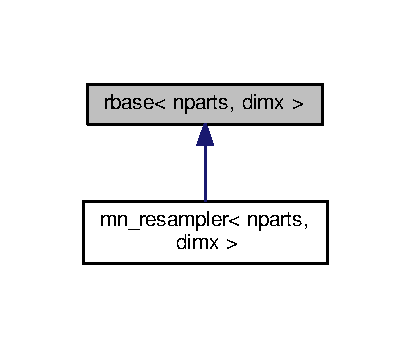
\includegraphics[width=350pt]{classrbase__inherit__graph}
\end{center}
\end{figure}
\subsection*{Public Types}
\begin{DoxyCompactItemize}
\item 
using \hyperlink{classrbase_ae20e0b8df15aa109252f57ecbf1f20f8}{ssv} = Eigen\+::\+Matrix$<$ float\+\_\+t, dimx, 1 $>$
\item 
using \hyperlink{classrbase_aa12fc826befa6ba0647b5f59ebc396ee}{array\+Vec} = std\+::array$<$ \hyperlink{classrbase_ae20e0b8df15aa109252f57ecbf1f20f8}{ssv}, nparts $>$
\item 
using \hyperlink{classrbase_a6f76bef853e508cb5b6f546d231b06f5}{array\+Float} = std\+::array$<$ float\+\_\+t, nparts $>$
\end{DoxyCompactItemize}
\subsection*{Public Member Functions}
\begin{DoxyCompactItemize}
\item 
\mbox{\Hypertarget{classrbase_aae80801bfc60ee3573cb728fc9460b0c}\label{classrbase_aae80801bfc60ee3573cb728fc9460b0c}} 
\hyperlink{classrbase_aae80801bfc60ee3573cb728fc9460b0c}{rbase} ()
\begin{DoxyCompactList}\small\item\em The default constructor gets called by default, and it sets the seed with the clock. \end{DoxyCompactList}\item 
virtual void \hyperlink{classrbase_aff0f6f88fd4656e67f5ebc870f10dd44}{resamp\+Log\+Wts} (\hyperlink{classrbase_aa12fc826befa6ba0647b5f59ebc396ee}{array\+Vec} \&old\+Parts, \hyperlink{classrbase_a6f76bef853e508cb5b6f546d231b06f5}{array\+Float} \&old\+Log\+Un\+Norm\+Wts)=0
\begin{DoxyCompactList}\small\item\em Function to resample from log unnormalized weights. \end{DoxyCompactList}\end{DoxyCompactItemize}
\subsection*{Protected Attributes}
\begin{DoxyCompactItemize}
\item 
\mbox{\Hypertarget{classrbase_ac278c975bd5b23ad009f1ce685552c5c}\label{classrbase_ac278c975bd5b23ad009f1ce685552c5c}} 
std\+::mt19937 \hyperlink{classrbase_ac278c975bd5b23ad009f1ce685552c5c}{m\+\_\+gen}
\begin{DoxyCompactList}\small\item\em prng \end{DoxyCompactList}\end{DoxyCompactItemize}


\subsection{Detailed Description}
\subsubsection*{template$<$size\+\_\+t nparts, size\+\_\+t dimx, typename float\+\_\+t$>$\newline
class rbase$<$ nparts, dimx, float\+\_\+t $>$}

Base class for all resampler types. 

\begin{DoxyAuthor}{Author}
taylor 
\end{DoxyAuthor}
\begin{DoxyDate}{Date}
15/04/18 
\end{DoxyDate}


\subsection{Member Typedef Documentation}
\mbox{\Hypertarget{classrbase_a6f76bef853e508cb5b6f546d231b06f5}\label{classrbase_a6f76bef853e508cb5b6f546d231b06f5}} 
\index{rbase@{rbase}!array\+Float@{array\+Float}}
\index{array\+Float@{array\+Float}!rbase@{rbase}}
\subsubsection{\texorpdfstring{array\+Float}{arrayFloat}}
{\footnotesize\ttfamily template$<$size\+\_\+t nparts, size\+\_\+t dimx, typename float\+\_\+t $>$ \\
using \hyperlink{classrbase}{rbase}$<$ nparts, dimx, float\+\_\+t $>$\+::\hyperlink{classrbase_a6f76bef853e508cb5b6f546d231b06f5}{array\+Float} =  std\+::array$<$float\+\_\+t,nparts$>$}

type alias for array of float\+\_\+ts \mbox{\Hypertarget{classrbase_aa12fc826befa6ba0647b5f59ebc396ee}\label{classrbase_aa12fc826befa6ba0647b5f59ebc396ee}} 
\index{rbase@{rbase}!array\+Vec@{array\+Vec}}
\index{array\+Vec@{array\+Vec}!rbase@{rbase}}
\subsubsection{\texorpdfstring{array\+Vec}{arrayVec}}
{\footnotesize\ttfamily template$<$size\+\_\+t nparts, size\+\_\+t dimx, typename float\+\_\+t $>$ \\
using \hyperlink{classrbase}{rbase}$<$ nparts, dimx, float\+\_\+t $>$\+::\hyperlink{classrbase_aa12fc826befa6ba0647b5f59ebc396ee}{array\+Vec} =  std\+::array$<$\hyperlink{classrbase_ae20e0b8df15aa109252f57ecbf1f20f8}{ssv}, nparts$>$}

type alias for array of Eigen Matrices \mbox{\Hypertarget{classrbase_ae20e0b8df15aa109252f57ecbf1f20f8}\label{classrbase_ae20e0b8df15aa109252f57ecbf1f20f8}} 
\index{rbase@{rbase}!ssv@{ssv}}
\index{ssv@{ssv}!rbase@{rbase}}
\subsubsection{\texorpdfstring{ssv}{ssv}}
{\footnotesize\ttfamily template$<$size\+\_\+t nparts, size\+\_\+t dimx, typename float\+\_\+t $>$ \\
using \hyperlink{classrbase}{rbase}$<$ nparts, dimx, float\+\_\+t $>$\+::\hyperlink{classrbase_ae20e0b8df15aa109252f57ecbf1f20f8}{ssv} =  Eigen\+::\+Matrix$<$float\+\_\+t,dimx,1$>$}

type alias for linear algebra stuff 

\subsection{Member Function Documentation}
\mbox{\Hypertarget{classrbase_aff0f6f88fd4656e67f5ebc870f10dd44}\label{classrbase_aff0f6f88fd4656e67f5ebc870f10dd44}} 
\index{rbase@{rbase}!resamp\+Log\+Wts@{resamp\+Log\+Wts}}
\index{resamp\+Log\+Wts@{resamp\+Log\+Wts}!rbase@{rbase}}
\subsubsection{\texorpdfstring{resamp\+Log\+Wts()}{resampLogWts()}}
{\footnotesize\ttfamily template$<$size\+\_\+t nparts, size\+\_\+t dimx, typename float\+\_\+t $>$ \\
virtual void \hyperlink{classrbase}{rbase}$<$ nparts, dimx, float\+\_\+t $>$\+::resamp\+Log\+Wts (\begin{DoxyParamCaption}\item[{\hyperlink{classrbase_aa12fc826befa6ba0647b5f59ebc396ee}{array\+Vec} \&}]{old\+Parts,  }\item[{\hyperlink{classrbase_a6f76bef853e508cb5b6f546d231b06f5}{array\+Float} \&}]{old\+Log\+Un\+Norm\+Wts }\end{DoxyParamCaption})\hspace{0.3cm}{\ttfamily [pure virtual]}}



Function to resample from log unnormalized weights. 


\begin{DoxyParams}{Parameters}
{\em old\+Parts} & \\
\hline
{\em old\+Log\+Un\+Norm\+Wts} & \\
\hline
\end{DoxyParams}


Implemented in \hyperlink{classmn__resamp__fast1_a398e64faa29bafd345c0258ca90d489c}{mn\+\_\+resamp\+\_\+fast1$<$ nparts, dimx, float\+\_\+t $>$}, \hyperlink{classsystematic__resampler_a9467aec6002043f35f40e9e4857021ed}{systematic\+\_\+resampler$<$ nparts, dimx, float\+\_\+t $>$}, \hyperlink{classstratif__resampler_a2588147563bf3fe598e262cae7e125e6}{stratif\+\_\+resampler$<$ nparts, dimx, float\+\_\+t $>$}, \hyperlink{classresid__resampler_ae6957cd1e080ac4313e6b0bc5ae9aa96}{resid\+\_\+resampler$<$ nparts, dimx, float\+\_\+t $>$}, and \hyperlink{classmn__resampler_a13b1897e180a791a3a099d5d6329a125}{mn\+\_\+resampler$<$ nparts, dimx, float\+\_\+t $>$}.



The documentation for this class was generated from the following file\+:\begin{DoxyCompactItemize}
\item 
include/pf/\hyperlink{resamplers_8h}{resamplers.\+h}\end{DoxyCompactItemize}

\hypertarget{classrvsamp__base}{}\section{rvsamp\+\_\+base$<$ dim $>$ Class Template Reference}
\label{classrvsamp__base}\index{rvsamp\+\_\+base$<$ dim $>$@{rvsamp\+\_\+base$<$ dim $>$}}


Base class for all random variable sampler types. Primary benefit is that it sets the seed for you.  




{\ttfamily \#include $<$rv\+\_\+samp.\+h$>$}



Inheritance diagram for rvsamp\+\_\+base$<$ dim $>$\+:\nopagebreak
\begin{figure}[H]
\begin{center}
\leavevmode
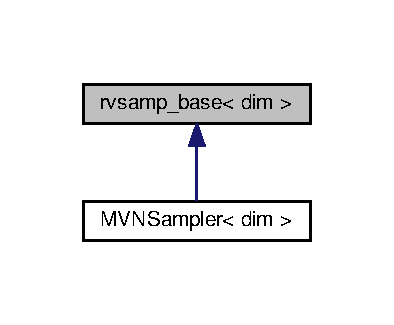
\includegraphics[width=189pt]{classrvsamp__base__inherit__graph}
\end{center}
\end{figure}
\subsection*{Public Types}
\begin{DoxyCompactItemize}
\item 
using \hyperlink{classrvsamp__base_a744275f57e806e6c787e331241b306eb}{ssv} = Eigen\+::\+Matrix$<$ double, dim, 1 $>$
\end{DoxyCompactItemize}
\subsection*{Public Member Functions}
\begin{DoxyCompactItemize}
\item 
\hyperlink{classrvsamp__base_a57fd1e9639c741bf464555756840daf2}{rvsamp\+\_\+base} ()\hypertarget{classrvsamp__base_a57fd1e9639c741bf464555756840daf2}{}\label{classrvsamp__base_a57fd1e9639c741bf464555756840daf2}

\begin{DoxyCompactList}\small\item\em The default constructor. This is the only option available. Sets the seed with the clock. \end{DoxyCompactList}\end{DoxyCompactItemize}
\subsection*{Protected Attributes}
\begin{DoxyCompactItemize}
\item 
std\+::mt19937 \hyperlink{classrvsamp__base_aa3df1440582518e6da779499728cac3c}{m\+\_\+rng}\hypertarget{classrvsamp__base_aa3df1440582518e6da779499728cac3c}{}\label{classrvsamp__base_aa3df1440582518e6da779499728cac3c}

\begin{DoxyCompactList}\small\item\em prng \end{DoxyCompactList}\end{DoxyCompactItemize}


\subsection{Detailed Description}
\subsubsection*{template$<$size\+\_\+t dim = 1$>$\\*
class rvsamp\+\_\+base$<$ dim $>$}

Base class for all random variable sampler types. Primary benefit is that it sets the seed for you. 

\begin{DoxyAuthor}{Author}
taylor 
\end{DoxyAuthor}


\subsection{Member Typedef Documentation}
\index{rvsamp\+\_\+base@{rvsamp\+\_\+base}!ssv@{ssv}}
\index{ssv@{ssv}!rvsamp\+\_\+base@{rvsamp\+\_\+base}}
\subsubsection[{\texorpdfstring{ssv}{ssv}}]{\setlength{\rightskip}{0pt plus 5cm}template$<$size\+\_\+t dim = 1$>$ using {\bf rvsamp\+\_\+base}$<$ dim $>$\+::{\bf ssv} =  Eigen\+::\+Matrix$<$double,dim,1$>$}\hypertarget{classrvsamp__base_a744275f57e806e6c787e331241b306eb}{}\label{classrvsamp__base_a744275f57e806e6c787e331241b306eb}
\char`\"{}state size vector\char`\"{} type alias for linear algebra stuff 

The documentation for this class was generated from the following file\+:\begin{DoxyCompactItemize}
\item 
include/\hyperlink{rv__samp_8h}{rv\+\_\+samp.\+h}\end{DoxyCompactItemize}

\hypertarget{classSISRFilter}{}\section{S\+I\+S\+R\+Filter$<$ nparts, dimx, dimy, resamp\+\_\+t, float\+\_\+t $>$ Class Template Reference}
\label{classSISRFilter}\index{S\+I\+S\+R\+Filter$<$ nparts, dimx, dimy, resamp\+\_\+t, float\+\_\+t $>$@{S\+I\+S\+R\+Filter$<$ nparts, dimx, dimy, resamp\+\_\+t, float\+\_\+t $>$}}


A base class for the Sequential Important Sampling with Resampling (S\+I\+SR).  




{\ttfamily \#include $<$sisr\+\_\+filter.\+h$>$}



Inheritance diagram for S\+I\+S\+R\+Filter$<$ nparts, dimx, dimy, resamp\+\_\+t, float\+\_\+t $>$\+:\nopagebreak
\begin{figure}[H]
\begin{center}
\leavevmode
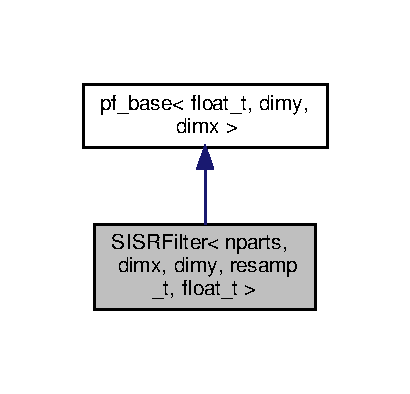
\includegraphics[width=197pt]{classSISRFilter__inherit__graph}
\end{center}
\end{figure}


Collaboration diagram for S\+I\+S\+R\+Filter$<$ nparts, dimx, dimy, resamp\+\_\+t, float\+\_\+t $>$\+:\nopagebreak
\begin{figure}[H]
\begin{center}
\leavevmode
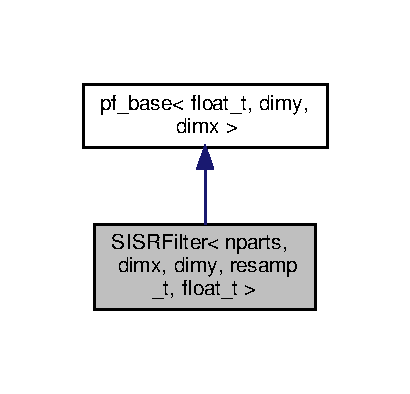
\includegraphics[width=197pt]{classSISRFilter__coll__graph}
\end{center}
\end{figure}
\subsection*{Public Types}
\begin{DoxyCompactItemize}
\item 
using \hyperlink{classSISRFilter_abfec45cf57ea6fadae4a9da8b0042351}{ssv} = Eigen\+::\+Matrix$<$ float\+\_\+t, dimx, 1 $>$
\item 
using \hyperlink{classSISRFilter_a5b762e9352857a9e48db3932191887ef}{osv} = Eigen\+::\+Matrix$<$ float\+\_\+t, dimy, 1 $>$
\item 
using \hyperlink{classSISRFilter_a7355e966778c788dfe227ef5254677c4}{Mat} = Eigen\+::\+Matrix$<$ float\+\_\+t, Eigen\+::\+Dynamic, Eigen\+::\+Dynamic $>$
\item 
using \hyperlink{classSISRFilter_a5c8a38ceb31c22f3c3f38b0ead5c1ce7}{array\+States} = std\+::array$<$ \hyperlink{classSISRFilter_abfec45cf57ea6fadae4a9da8b0042351}{ssv}, nparts $>$
\item 
using \hyperlink{classSISRFilter_a35f5a590324bd78fc4f6ded236937ac2}{arrayfloat\+\_\+t} = std\+::array$<$ float\+\_\+t, nparts $>$
\end{DoxyCompactItemize}
\subsection*{Public Member Functions}
\begin{DoxyCompactItemize}
\item 
\hyperlink{classSISRFilter_a46243d4a5ef93f3762d1130fa4d43389}{S\+I\+S\+R\+Filter} (const unsigned int \&rs=1)
\begin{DoxyCompactList}\small\item\em The (one and only) constructor. \end{DoxyCompactList}\item 
\mbox{\Hypertarget{classSISRFilter_a0934886c2ab47682364e3624c24be874}\label{classSISRFilter_a0934886c2ab47682364e3624c24be874}} 
virtual \hyperlink{classSISRFilter_a0934886c2ab47682364e3624c24be874}{$\sim$\+S\+I\+S\+R\+Filter} ()
\begin{DoxyCompactList}\small\item\em The (virtual) destructor. \end{DoxyCompactList}\item 
float\+\_\+t \hyperlink{classSISRFilter_a48bdb88b2ed4041ab6d8a6547703ebf3}{get\+Log\+Cond\+Like} () const
\begin{DoxyCompactList}\small\item\em Returns the most recent (log-\/) conditiona likelihood. \end{DoxyCompactList}\item 
std\+::vector$<$ \hyperlink{classSISRFilter_a7355e966778c788dfe227ef5254677c4}{Mat} $>$ \hyperlink{classSISRFilter_a88ef9409ded3ec7e6745e184daad86c4}{get\+Expectations} () const
\begin{DoxyCompactList}\small\item\em return all stored expectations (taken with respect to \$p(x\+\_\+t$\vert$y\+\_\+\{1\+:t\})\$ \end{DoxyCompactList}\item 
void \hyperlink{classSISRFilter_a0fd4ac5135ff9a4bb32a286533855197}{filter} (const \hyperlink{classSISRFilter_a5b762e9352857a9e48db3932191887ef}{osv} \&data, const std\+::vector$<$ std\+::function$<$ const \hyperlink{classSISRFilter_a7355e966778c788dfe227ef5254677c4}{Mat}(const \hyperlink{classSISRFilter_abfec45cf57ea6fadae4a9da8b0042351}{ssv} \&)$>$ $>$ \&fs=std\+::vector$<$ std\+::function$<$ const \hyperlink{classSISRFilter_a7355e966778c788dfe227ef5254677c4}{Mat}(const \hyperlink{classSISRFilter_abfec45cf57ea6fadae4a9da8b0042351}{ssv} \&)$>$ $>$())
\begin{DoxyCompactList}\small\item\em updates filtering distribution on a new datapoint. Optionally stores expectations of functionals. \end{DoxyCompactList}\item 
virtual float\+\_\+t \hyperlink{classSISRFilter_aff620e2208b6b26bbe109ce05520c5f8}{log\+Mu\+Ev} (const \hyperlink{classSISRFilter_abfec45cf57ea6fadae4a9da8b0042351}{ssv} \&x1)=0
\begin{DoxyCompactList}\small\item\em Calculate mu\+Ev or logmu\+Ev. \end{DoxyCompactList}\item 
virtual \hyperlink{classSISRFilter_abfec45cf57ea6fadae4a9da8b0042351}{ssv} \hyperlink{classSISRFilter_aac34adbf022dad8b62470de35c5ceb17}{q1\+Samp} (const \hyperlink{classSISRFilter_a5b762e9352857a9e48db3932191887ef}{osv} \&y1)=0
\begin{DoxyCompactList}\small\item\em Samples from time 1 proposal. \end{DoxyCompactList}\item 
virtual float\+\_\+t \hyperlink{classSISRFilter_a21d5130f35d1d5c21b697ca7ea8e9d83}{log\+Q1\+Ev} (const \hyperlink{classSISRFilter_abfec45cf57ea6fadae4a9da8b0042351}{ssv} \&x1, const \hyperlink{classSISRFilter_a5b762e9352857a9e48db3932191887ef}{osv} \&y1)=0
\begin{DoxyCompactList}\small\item\em Calculate q1\+Ev or log q1\+Ev. \end{DoxyCompactList}\item 
virtual float\+\_\+t \hyperlink{classSISRFilter_a73fe8481e4cb40142544c04823851aa8}{log\+G\+Ev} (const \hyperlink{classSISRFilter_a5b762e9352857a9e48db3932191887ef}{osv} \&yt, const \hyperlink{classSISRFilter_abfec45cf57ea6fadae4a9da8b0042351}{ssv} \&xt)=0
\begin{DoxyCompactList}\small\item\em Calculate g\+Ev or log\+G\+Ev. \end{DoxyCompactList}\item 
virtual float\+\_\+t \hyperlink{classSISRFilter_a7aa1e90a0b641728d5f8d7bd8c699ba8}{log\+F\+Ev} (const \hyperlink{classSISRFilter_abfec45cf57ea6fadae4a9da8b0042351}{ssv} \&xt, const \hyperlink{classSISRFilter_abfec45cf57ea6fadae4a9da8b0042351}{ssv} \&xtm1)=0
\begin{DoxyCompactList}\small\item\em Evaluates the state transition density. \end{DoxyCompactList}\item 
virtual \hyperlink{classSISRFilter_abfec45cf57ea6fadae4a9da8b0042351}{ssv} \hyperlink{classSISRFilter_a609bb361da16e1b24ebfab693620241b}{q\+Samp} (const \hyperlink{classSISRFilter_abfec45cf57ea6fadae4a9da8b0042351}{ssv} \&xtm1, const \hyperlink{classSISRFilter_a5b762e9352857a9e48db3932191887ef}{osv} \&yt)=0
\begin{DoxyCompactList}\small\item\em Samples from the proposal/instrumental/importance density at time t. \end{DoxyCompactList}\item 
virtual float\+\_\+t \hyperlink{classSISRFilter_a4edca9291a3a118c37bd0e41c06fb7da}{log\+Q\+Ev} (const \hyperlink{classSISRFilter_abfec45cf57ea6fadae4a9da8b0042351}{ssv} \&xt, const \hyperlink{classSISRFilter_abfec45cf57ea6fadae4a9da8b0042351}{ssv} \&xtm1, const \hyperlink{classSISRFilter_a5b762e9352857a9e48db3932191887ef}{osv} \&yt)=0
\begin{DoxyCompactList}\small\item\em Evaluates the proposal/instrumental/importance density/pmf. \end{DoxyCompactList}\end{DoxyCompactItemize}
\subsection*{Private Attributes}
\begin{DoxyCompactItemize}
\item 
\mbox{\Hypertarget{classSISRFilter_a98c87c50c054354cdc85dc800ba15bdd}\label{classSISRFilter_a98c87c50c054354cdc85dc800ba15bdd}} 
\hyperlink{classSISRFilter_a5c8a38ceb31c22f3c3f38b0ead5c1ce7}{array\+States} \hyperlink{classSISRFilter_a98c87c50c054354cdc85dc800ba15bdd}{m\+\_\+particles}
\begin{DoxyCompactList}\small\item\em particle samples \end{DoxyCompactList}\item 
\mbox{\Hypertarget{classSISRFilter_a99f63cbae203084cf3d812a61bb725fe}\label{classSISRFilter_a99f63cbae203084cf3d812a61bb725fe}} 
\hyperlink{classSISRFilter_a35f5a590324bd78fc4f6ded236937ac2}{arrayfloat\+\_\+t} \hyperlink{classSISRFilter_a99f63cbae203084cf3d812a61bb725fe}{m\+\_\+log\+Un\+Norm\+Weights}
\begin{DoxyCompactList}\small\item\em particle weights \end{DoxyCompactList}\item 
\mbox{\Hypertarget{classSISRFilter_a1aafd7da52826fd25967c8258f68ce9c}\label{classSISRFilter_a1aafd7da52826fd25967c8258f68ce9c}} 
unsigned int \hyperlink{classSISRFilter_a1aafd7da52826fd25967c8258f68ce9c}{m\+\_\+now}
\begin{DoxyCompactList}\small\item\em current time point \end{DoxyCompactList}\item 
\mbox{\Hypertarget{classSISRFilter_a7031db4bd7d9c1db7ea83150893525ed}\label{classSISRFilter_a7031db4bd7d9c1db7ea83150893525ed}} 
float\+\_\+t \hyperlink{classSISRFilter_a7031db4bd7d9c1db7ea83150893525ed}{m\+\_\+log\+Last\+Cond\+Like}
\begin{DoxyCompactList}\small\item\em log p(y\+\_\+t$\vert$y\+\_\+\{1\+:t-\/1\}) or log p(y1) \end{DoxyCompactList}\item 
\mbox{\Hypertarget{classSISRFilter_a46f945e550fab93eedddf10a69c251f1}\label{classSISRFilter_a46f945e550fab93eedddf10a69c251f1}} 
resamp\+\_\+t \hyperlink{classSISRFilter_a46f945e550fab93eedddf10a69c251f1}{m\+\_\+resampler}
\begin{DoxyCompactList}\small\item\em resampling object \end{DoxyCompactList}\item 
\mbox{\Hypertarget{classSISRFilter_acb5ed65aeed970afb929c108d04ee0d1}\label{classSISRFilter_acb5ed65aeed970afb929c108d04ee0d1}} 
std\+::vector$<$ \hyperlink{classSISRFilter_a7355e966778c788dfe227ef5254677c4}{Mat} $>$ \hyperlink{classSISRFilter_acb5ed65aeed970afb929c108d04ee0d1}{m\+\_\+expectations}
\begin{DoxyCompactList}\small\item\em expectations E\mbox{[}h(x\+\_\+t) $\vert$ y\+\_\+\{1\+:t\}\mbox{]} for user defined \char`\"{}h\char`\"{}s \end{DoxyCompactList}\item 
\mbox{\Hypertarget{classSISRFilter_a196049324b4c6c42a927d83f659619aa}\label{classSISRFilter_a196049324b4c6c42a927d83f659619aa}} 
unsigned int \hyperlink{classSISRFilter_a196049324b4c6c42a927d83f659619aa}{m\+\_\+resamp\+Sched}
\begin{DoxyCompactList}\small\item\em resampling schedule (e.\+g. resample every \+\_\+\+\_\+ time points) \end{DoxyCompactList}\end{DoxyCompactItemize}


\subsection{Detailed Description}
\subsubsection*{template$<$size\+\_\+t nparts, size\+\_\+t dimx, size\+\_\+t dimy, typename resamp\+\_\+t, typename float\+\_\+t$>$\newline
class S\+I\+S\+R\+Filter$<$ nparts, dimx, dimy, resamp\+\_\+t, float\+\_\+t $>$}

A base class for the Sequential Important Sampling with Resampling (S\+I\+SR). 

\begin{DoxyAuthor}{Author}
taylor 
\end{DoxyAuthor}


\subsection{Member Typedef Documentation}
\mbox{\Hypertarget{classSISRFilter_a35f5a590324bd78fc4f6ded236937ac2}\label{classSISRFilter_a35f5a590324bd78fc4f6ded236937ac2}} 
\index{S\+I\+S\+R\+Filter@{S\+I\+S\+R\+Filter}!arrayfloat\+\_\+t@{arrayfloat\+\_\+t}}
\index{arrayfloat\+\_\+t@{arrayfloat\+\_\+t}!S\+I\+S\+R\+Filter@{S\+I\+S\+R\+Filter}}
\subsubsection{\texorpdfstring{arrayfloat\+\_\+t}{arrayfloat\_t}}
{\footnotesize\ttfamily template$<$size\+\_\+t nparts, size\+\_\+t dimx, size\+\_\+t dimy, typename resamp\+\_\+t , typename float\+\_\+t $>$ \\
using \hyperlink{classSISRFilter}{S\+I\+S\+R\+Filter}$<$ nparts, dimx, dimy, resamp\+\_\+t, float\+\_\+t $>$\+::\hyperlink{classSISRFilter_a35f5a590324bd78fc4f6ded236937ac2}{arrayfloat\+\_\+t} =  std\+::array$<$float\+\_\+t, nparts$>$}

type alias for array of float\+\_\+ts \mbox{\Hypertarget{classSISRFilter_a5c8a38ceb31c22f3c3f38b0ead5c1ce7}\label{classSISRFilter_a5c8a38ceb31c22f3c3f38b0ead5c1ce7}} 
\index{S\+I\+S\+R\+Filter@{S\+I\+S\+R\+Filter}!array\+States@{array\+States}}
\index{array\+States@{array\+States}!S\+I\+S\+R\+Filter@{S\+I\+S\+R\+Filter}}
\subsubsection{\texorpdfstring{array\+States}{arrayStates}}
{\footnotesize\ttfamily template$<$size\+\_\+t nparts, size\+\_\+t dimx, size\+\_\+t dimy, typename resamp\+\_\+t , typename float\+\_\+t $>$ \\
using \hyperlink{classSISRFilter}{S\+I\+S\+R\+Filter}$<$ nparts, dimx, dimy, resamp\+\_\+t, float\+\_\+t $>$\+::\hyperlink{classSISRFilter_a5c8a38ceb31c22f3c3f38b0ead5c1ce7}{array\+States} =  std\+::array$<$\hyperlink{classSISRFilter_abfec45cf57ea6fadae4a9da8b0042351}{ssv}, nparts$>$}

type alias for linear algebra stuff \mbox{\Hypertarget{classSISRFilter_a7355e966778c788dfe227ef5254677c4}\label{classSISRFilter_a7355e966778c788dfe227ef5254677c4}} 
\index{S\+I\+S\+R\+Filter@{S\+I\+S\+R\+Filter}!Mat@{Mat}}
\index{Mat@{Mat}!S\+I\+S\+R\+Filter@{S\+I\+S\+R\+Filter}}
\subsubsection{\texorpdfstring{Mat}{Mat}}
{\footnotesize\ttfamily template$<$size\+\_\+t nparts, size\+\_\+t dimx, size\+\_\+t dimy, typename resamp\+\_\+t , typename float\+\_\+t $>$ \\
using \hyperlink{classSISRFilter}{S\+I\+S\+R\+Filter}$<$ nparts, dimx, dimy, resamp\+\_\+t, float\+\_\+t $>$\+::\hyperlink{classSISRFilter_a7355e966778c788dfe227ef5254677c4}{Mat} =  Eigen\+::\+Matrix$<$float\+\_\+t,Eigen\+::\+Dynamic,Eigen\+::\+Dynamic$>$}

type alias for linear algebra stuff \mbox{\Hypertarget{classSISRFilter_a5b762e9352857a9e48db3932191887ef}\label{classSISRFilter_a5b762e9352857a9e48db3932191887ef}} 
\index{S\+I\+S\+R\+Filter@{S\+I\+S\+R\+Filter}!osv@{osv}}
\index{osv@{osv}!S\+I\+S\+R\+Filter@{S\+I\+S\+R\+Filter}}
\subsubsection{\texorpdfstring{osv}{osv}}
{\footnotesize\ttfamily template$<$size\+\_\+t nparts, size\+\_\+t dimx, size\+\_\+t dimy, typename resamp\+\_\+t , typename float\+\_\+t $>$ \\
using \hyperlink{classSISRFilter}{S\+I\+S\+R\+Filter}$<$ nparts, dimx, dimy, resamp\+\_\+t, float\+\_\+t $>$\+::\hyperlink{classSISRFilter_a5b762e9352857a9e48db3932191887ef}{osv} =  Eigen\+::\+Matrix$<$float\+\_\+t, dimy, 1$>$}

\char`\"{}obs size vector\char`\"{} type alias for linear algebra stuff \mbox{\Hypertarget{classSISRFilter_abfec45cf57ea6fadae4a9da8b0042351}\label{classSISRFilter_abfec45cf57ea6fadae4a9da8b0042351}} 
\index{S\+I\+S\+R\+Filter@{S\+I\+S\+R\+Filter}!ssv@{ssv}}
\index{ssv@{ssv}!S\+I\+S\+R\+Filter@{S\+I\+S\+R\+Filter}}
\subsubsection{\texorpdfstring{ssv}{ssv}}
{\footnotesize\ttfamily template$<$size\+\_\+t nparts, size\+\_\+t dimx, size\+\_\+t dimy, typename resamp\+\_\+t , typename float\+\_\+t $>$ \\
using \hyperlink{classSISRFilter}{S\+I\+S\+R\+Filter}$<$ nparts, dimx, dimy, resamp\+\_\+t, float\+\_\+t $>$\+::\hyperlink{classSISRFilter_abfec45cf57ea6fadae4a9da8b0042351}{ssv} =  Eigen\+::\+Matrix$<$float\+\_\+t, dimx, 1$>$}

\char`\"{}state size vector\char`\"{} type alias for linear algebra stuff 

\subsection{Constructor \& Destructor Documentation}
\mbox{\Hypertarget{classSISRFilter_a46243d4a5ef93f3762d1130fa4d43389}\label{classSISRFilter_a46243d4a5ef93f3762d1130fa4d43389}} 
\index{S\+I\+S\+R\+Filter@{S\+I\+S\+R\+Filter}!S\+I\+S\+R\+Filter@{S\+I\+S\+R\+Filter}}
\index{S\+I\+S\+R\+Filter@{S\+I\+S\+R\+Filter}!S\+I\+S\+R\+Filter@{S\+I\+S\+R\+Filter}}
\subsubsection{\texorpdfstring{S\+I\+S\+R\+Filter()}{SISRFilter()}}
{\footnotesize\ttfamily template$<$size\+\_\+t nparts, size\+\_\+t dimx, size\+\_\+t dimy, typename resamp\+\_\+t , typename float\+\_\+t $>$ \\
\hyperlink{classSISRFilter}{S\+I\+S\+R\+Filter}$<$ nparts, dimx, dimy, resamp\+\_\+t, float\+\_\+t $>$\+::\hyperlink{classSISRFilter}{S\+I\+S\+R\+Filter} (\begin{DoxyParamCaption}\item[{const unsigned int \&}]{rs = {\ttfamily 1} }\end{DoxyParamCaption})}



The (one and only) constructor. 


\begin{DoxyParams}{Parameters}
{\em rs} & the resampling schedule (resample every rs time points). \\
\hline
\end{DoxyParams}


\subsection{Member Function Documentation}
\mbox{\Hypertarget{classSISRFilter_a0fd4ac5135ff9a4bb32a286533855197}\label{classSISRFilter_a0fd4ac5135ff9a4bb32a286533855197}} 
\index{S\+I\+S\+R\+Filter@{S\+I\+S\+R\+Filter}!filter@{filter}}
\index{filter@{filter}!S\+I\+S\+R\+Filter@{S\+I\+S\+R\+Filter}}
\subsubsection{\texorpdfstring{filter()}{filter()}}
{\footnotesize\ttfamily template$<$size\+\_\+t nparts, size\+\_\+t dimx, size\+\_\+t dimy, typename resamp\+\_\+t , typename float\+\_\+t $>$ \\
void \hyperlink{classSISRFilter}{S\+I\+S\+R\+Filter}$<$ nparts, dimx, dimy, resamp\+\_\+t, float\+\_\+t $>$\+::filter (\begin{DoxyParamCaption}\item[{const \hyperlink{classSISRFilter_a5b762e9352857a9e48db3932191887ef}{osv} \&}]{data,  }\item[{const std\+::vector$<$ std\+::function$<$ const \hyperlink{classSISRFilter_a7355e966778c788dfe227ef5254677c4}{Mat}(const \hyperlink{classSISRFilter_abfec45cf57ea6fadae4a9da8b0042351}{ssv} \&)$>$ $>$ \&}]{fs = {\ttfamily std\+:\+:vector$<$std\+:\+:function$<$const~\hyperlink{classSISRFilter_a7355e966778c788dfe227ef5254677c4}{Mat}(const~\hyperlink{classSISRFilter_abfec45cf57ea6fadae4a9da8b0042351}{ssv}\&)$>$~$>$()} }\end{DoxyParamCaption})}



updates filtering distribution on a new datapoint. Optionally stores expectations of functionals. 


\begin{DoxyParams}{Parameters}
{\em data} & the most recent data point \\
\hline
{\em fs} & a vector of functions if you want to calculate expectations. \\
\hline
\end{DoxyParams}
\mbox{\Hypertarget{classSISRFilter_a88ef9409ded3ec7e6745e184daad86c4}\label{classSISRFilter_a88ef9409ded3ec7e6745e184daad86c4}} 
\index{S\+I\+S\+R\+Filter@{S\+I\+S\+R\+Filter}!get\+Expectations@{get\+Expectations}}
\index{get\+Expectations@{get\+Expectations}!S\+I\+S\+R\+Filter@{S\+I\+S\+R\+Filter}}
\subsubsection{\texorpdfstring{get\+Expectations()}{getExpectations()}}
{\footnotesize\ttfamily template$<$size\+\_\+t nparts, size\+\_\+t dimx, size\+\_\+t dimy, typename resamp\+\_\+t , typename float\+\_\+t $>$ \\
auto \hyperlink{classSISRFilter}{S\+I\+S\+R\+Filter}$<$ nparts, dimx, dimy, resamp\+\_\+t, float\+\_\+t $>$\+::get\+Expectations (\begin{DoxyParamCaption}{ }\end{DoxyParamCaption}) const}



return all stored expectations (taken with respect to \$p(x\+\_\+t$\vert$y\+\_\+\{1\+:t\})\$ 

\begin{DoxyReturn}{Returns}
return a std\+::vector$<$\+Mat$>$ of expectations. How many depends on how many callbacks you gave to 
\end{DoxyReturn}
\mbox{\Hypertarget{classSISRFilter_a48bdb88b2ed4041ab6d8a6547703ebf3}\label{classSISRFilter_a48bdb88b2ed4041ab6d8a6547703ebf3}} 
\index{S\+I\+S\+R\+Filter@{S\+I\+S\+R\+Filter}!get\+Log\+Cond\+Like@{get\+Log\+Cond\+Like}}
\index{get\+Log\+Cond\+Like@{get\+Log\+Cond\+Like}!S\+I\+S\+R\+Filter@{S\+I\+S\+R\+Filter}}
\subsubsection{\texorpdfstring{get\+Log\+Cond\+Like()}{getLogCondLike()}}
{\footnotesize\ttfamily template$<$size\+\_\+t nparts, size\+\_\+t dimx, size\+\_\+t dimy, typename resamp\+\_\+t , typename float\+\_\+t $>$ \\
float\+\_\+t \hyperlink{classSISRFilter}{S\+I\+S\+R\+Filter}$<$ nparts, dimx, dimy, resamp\+\_\+t, float\+\_\+t $>$\+::get\+Log\+Cond\+Like (\begin{DoxyParamCaption}{ }\end{DoxyParamCaption}) const\hspace{0.3cm}{\ttfamily [virtual]}}



Returns the most recent (log-\/) conditiona likelihood. 

\begin{DoxyReturn}{Returns}
log p(y\+\_\+t $\vert$ y\+\_\+\{1\+:t-\/1\}) or log p(y\+\_\+1) 
\end{DoxyReturn}


Implements \hyperlink{classpf__base_a350df818820d6ab0fd6d413022b7f23b}{pf\+\_\+base$<$ float\+\_\+t, dimy, dimx $>$}.

\mbox{\Hypertarget{classSISRFilter_a7aa1e90a0b641728d5f8d7bd8c699ba8}\label{classSISRFilter_a7aa1e90a0b641728d5f8d7bd8c699ba8}} 
\index{S\+I\+S\+R\+Filter@{S\+I\+S\+R\+Filter}!log\+F\+Ev@{log\+F\+Ev}}
\index{log\+F\+Ev@{log\+F\+Ev}!S\+I\+S\+R\+Filter@{S\+I\+S\+R\+Filter}}
\subsubsection{\texorpdfstring{log\+F\+Ev()}{logFEv()}}
{\footnotesize\ttfamily template$<$size\+\_\+t nparts, size\+\_\+t dimx, size\+\_\+t dimy, typename resamp\+\_\+t , typename float\+\_\+t $>$ \\
virtual float\+\_\+t \hyperlink{classSISRFilter}{S\+I\+S\+R\+Filter}$<$ nparts, dimx, dimy, resamp\+\_\+t, float\+\_\+t $>$\+::log\+F\+Ev (\begin{DoxyParamCaption}\item[{const \hyperlink{classSISRFilter_abfec45cf57ea6fadae4a9da8b0042351}{ssv} \&}]{xt,  }\item[{const \hyperlink{classSISRFilter_abfec45cf57ea6fadae4a9da8b0042351}{ssv} \&}]{xtm1 }\end{DoxyParamCaption})\hspace{0.3cm}{\ttfamily [pure virtual]}}



Evaluates the state transition density. 


\begin{DoxyParams}{Parameters}
{\em xt} & the current state \\
\hline
{\em xtm1} & the previous state \\
\hline
\end{DoxyParams}
\begin{DoxyReturn}{Returns}
a float\+\_\+t evaluaton of the log density/pmf 
\end{DoxyReturn}
\mbox{\Hypertarget{classSISRFilter_a73fe8481e4cb40142544c04823851aa8}\label{classSISRFilter_a73fe8481e4cb40142544c04823851aa8}} 
\index{S\+I\+S\+R\+Filter@{S\+I\+S\+R\+Filter}!log\+G\+Ev@{log\+G\+Ev}}
\index{log\+G\+Ev@{log\+G\+Ev}!S\+I\+S\+R\+Filter@{S\+I\+S\+R\+Filter}}
\subsubsection{\texorpdfstring{log\+G\+Ev()}{logGEv()}}
{\footnotesize\ttfamily template$<$size\+\_\+t nparts, size\+\_\+t dimx, size\+\_\+t dimy, typename resamp\+\_\+t , typename float\+\_\+t $>$ \\
virtual float\+\_\+t \hyperlink{classSISRFilter}{S\+I\+S\+R\+Filter}$<$ nparts, dimx, dimy, resamp\+\_\+t, float\+\_\+t $>$\+::log\+G\+Ev (\begin{DoxyParamCaption}\item[{const \hyperlink{classSISRFilter_a5b762e9352857a9e48db3932191887ef}{osv} \&}]{yt,  }\item[{const \hyperlink{classSISRFilter_abfec45cf57ea6fadae4a9da8b0042351}{ssv} \&}]{xt }\end{DoxyParamCaption})\hspace{0.3cm}{\ttfamily [pure virtual]}}



Calculate g\+Ev or log\+G\+Ev. 


\begin{DoxyParams}{Parameters}
{\em yt} & is a const Vec\& describing the time t datum \\
\hline
{\em xt} & is a const Vec\& describing the time t state \\
\hline
\end{DoxyParams}
\begin{DoxyReturn}{Returns}
the density or log-\/density evaluation as a float\+\_\+t 
\end{DoxyReturn}
\mbox{\Hypertarget{classSISRFilter_aff620e2208b6b26bbe109ce05520c5f8}\label{classSISRFilter_aff620e2208b6b26bbe109ce05520c5f8}} 
\index{S\+I\+S\+R\+Filter@{S\+I\+S\+R\+Filter}!log\+Mu\+Ev@{log\+Mu\+Ev}}
\index{log\+Mu\+Ev@{log\+Mu\+Ev}!S\+I\+S\+R\+Filter@{S\+I\+S\+R\+Filter}}
\subsubsection{\texorpdfstring{log\+Mu\+Ev()}{logMuEv()}}
{\footnotesize\ttfamily template$<$size\+\_\+t nparts, size\+\_\+t dimx, size\+\_\+t dimy, typename resamp\+\_\+t , typename float\+\_\+t $>$ \\
virtual float\+\_\+t \hyperlink{classSISRFilter}{S\+I\+S\+R\+Filter}$<$ nparts, dimx, dimy, resamp\+\_\+t, float\+\_\+t $>$\+::log\+Mu\+Ev (\begin{DoxyParamCaption}\item[{const \hyperlink{classSISRFilter_abfec45cf57ea6fadae4a9da8b0042351}{ssv} \&}]{x1 }\end{DoxyParamCaption})\hspace{0.3cm}{\ttfamily [pure virtual]}}



Calculate mu\+Ev or logmu\+Ev. 


\begin{DoxyParams}{Parameters}
{\em x1} & is a const Vec\& describing the state sample \\
\hline
\end{DoxyParams}
\begin{DoxyReturn}{Returns}
the density or log-\/density evaluation as a float\+\_\+t 
\end{DoxyReturn}
\mbox{\Hypertarget{classSISRFilter_a21d5130f35d1d5c21b697ca7ea8e9d83}\label{classSISRFilter_a21d5130f35d1d5c21b697ca7ea8e9d83}} 
\index{S\+I\+S\+R\+Filter@{S\+I\+S\+R\+Filter}!log\+Q1\+Ev@{log\+Q1\+Ev}}
\index{log\+Q1\+Ev@{log\+Q1\+Ev}!S\+I\+S\+R\+Filter@{S\+I\+S\+R\+Filter}}
\subsubsection{\texorpdfstring{log\+Q1\+Ev()}{logQ1Ev()}}
{\footnotesize\ttfamily template$<$size\+\_\+t nparts, size\+\_\+t dimx, size\+\_\+t dimy, typename resamp\+\_\+t , typename float\+\_\+t $>$ \\
virtual float\+\_\+t \hyperlink{classSISRFilter}{S\+I\+S\+R\+Filter}$<$ nparts, dimx, dimy, resamp\+\_\+t, float\+\_\+t $>$\+::log\+Q1\+Ev (\begin{DoxyParamCaption}\item[{const \hyperlink{classSISRFilter_abfec45cf57ea6fadae4a9da8b0042351}{ssv} \&}]{x1,  }\item[{const \hyperlink{classSISRFilter_a5b762e9352857a9e48db3932191887ef}{osv} \&}]{y1 }\end{DoxyParamCaption})\hspace{0.3cm}{\ttfamily [pure virtual]}}



Calculate q1\+Ev or log q1\+Ev. 


\begin{DoxyParams}{Parameters}
{\em x1} & is a const Vec\& describing the time 1 state sample \\
\hline
{\em y1} & is a const Vec\& describing the time 1 datum \\
\hline
\end{DoxyParams}
\begin{DoxyReturn}{Returns}
the density or log-\/density evaluation as a float\+\_\+t 
\end{DoxyReturn}
\mbox{\Hypertarget{classSISRFilter_a4edca9291a3a118c37bd0e41c06fb7da}\label{classSISRFilter_a4edca9291a3a118c37bd0e41c06fb7da}} 
\index{S\+I\+S\+R\+Filter@{S\+I\+S\+R\+Filter}!log\+Q\+Ev@{log\+Q\+Ev}}
\index{log\+Q\+Ev@{log\+Q\+Ev}!S\+I\+S\+R\+Filter@{S\+I\+S\+R\+Filter}}
\subsubsection{\texorpdfstring{log\+Q\+Ev()}{logQEv()}}
{\footnotesize\ttfamily template$<$size\+\_\+t nparts, size\+\_\+t dimx, size\+\_\+t dimy, typename resamp\+\_\+t , typename float\+\_\+t $>$ \\
virtual float\+\_\+t \hyperlink{classSISRFilter}{S\+I\+S\+R\+Filter}$<$ nparts, dimx, dimy, resamp\+\_\+t, float\+\_\+t $>$\+::log\+Q\+Ev (\begin{DoxyParamCaption}\item[{const \hyperlink{classSISRFilter_abfec45cf57ea6fadae4a9da8b0042351}{ssv} \&}]{xt,  }\item[{const \hyperlink{classSISRFilter_abfec45cf57ea6fadae4a9da8b0042351}{ssv} \&}]{xtm1,  }\item[{const \hyperlink{classSISRFilter_a5b762e9352857a9e48db3932191887ef}{osv} \&}]{yt }\end{DoxyParamCaption})\hspace{0.3cm}{\ttfamily [pure virtual]}}



Evaluates the proposal/instrumental/importance density/pmf. 


\begin{DoxyParams}{Parameters}
{\em xt} & current state \\
\hline
{\em xtm1} & previous state \\
\hline
{\em yt} & current observation \\
\hline
\end{DoxyParams}
\begin{DoxyReturn}{Returns}
a float\+\_\+t evaluation of the log density/pmf 
\end{DoxyReturn}
\mbox{\Hypertarget{classSISRFilter_aac34adbf022dad8b62470de35c5ceb17}\label{classSISRFilter_aac34adbf022dad8b62470de35c5ceb17}} 
\index{S\+I\+S\+R\+Filter@{S\+I\+S\+R\+Filter}!q1\+Samp@{q1\+Samp}}
\index{q1\+Samp@{q1\+Samp}!S\+I\+S\+R\+Filter@{S\+I\+S\+R\+Filter}}
\subsubsection{\texorpdfstring{q1\+Samp()}{q1Samp()}}
{\footnotesize\ttfamily template$<$size\+\_\+t nparts, size\+\_\+t dimx, size\+\_\+t dimy, typename resamp\+\_\+t , typename float\+\_\+t $>$ \\
virtual \hyperlink{classSISRFilter_abfec45cf57ea6fadae4a9da8b0042351}{ssv} \hyperlink{classSISRFilter}{S\+I\+S\+R\+Filter}$<$ nparts, dimx, dimy, resamp\+\_\+t, float\+\_\+t $>$\+::q1\+Samp (\begin{DoxyParamCaption}\item[{const \hyperlink{classSISRFilter_a5b762e9352857a9e48db3932191887ef}{osv} \&}]{y1 }\end{DoxyParamCaption})\hspace{0.3cm}{\ttfamily [pure virtual]}}



Samples from time 1 proposal. 


\begin{DoxyParams}{Parameters}
{\em y1} & is a const Vec\& representing the first observed datum \\
\hline
\end{DoxyParams}
\begin{DoxyReturn}{Returns}
the sample as a Vec 
\end{DoxyReturn}
\mbox{\Hypertarget{classSISRFilter_a609bb361da16e1b24ebfab693620241b}\label{classSISRFilter_a609bb361da16e1b24ebfab693620241b}} 
\index{S\+I\+S\+R\+Filter@{S\+I\+S\+R\+Filter}!q\+Samp@{q\+Samp}}
\index{q\+Samp@{q\+Samp}!S\+I\+S\+R\+Filter@{S\+I\+S\+R\+Filter}}
\subsubsection{\texorpdfstring{q\+Samp()}{qSamp()}}
{\footnotesize\ttfamily template$<$size\+\_\+t nparts, size\+\_\+t dimx, size\+\_\+t dimy, typename resamp\+\_\+t , typename float\+\_\+t $>$ \\
virtual \hyperlink{classSISRFilter_abfec45cf57ea6fadae4a9da8b0042351}{ssv} \hyperlink{classSISRFilter}{S\+I\+S\+R\+Filter}$<$ nparts, dimx, dimy, resamp\+\_\+t, float\+\_\+t $>$\+::q\+Samp (\begin{DoxyParamCaption}\item[{const \hyperlink{classSISRFilter_abfec45cf57ea6fadae4a9da8b0042351}{ssv} \&}]{xtm1,  }\item[{const \hyperlink{classSISRFilter_a5b762e9352857a9e48db3932191887ef}{osv} \&}]{yt }\end{DoxyParamCaption})\hspace{0.3cm}{\ttfamily [pure virtual]}}



Samples from the proposal/instrumental/importance density at time t. 


\begin{DoxyParams}{Parameters}
{\em xtm1} & the previous state sample \\
\hline
{\em yt} & the current observation \\
\hline
\end{DoxyParams}
\begin{DoxyReturn}{Returns}
a state sample for the current time xt 
\end{DoxyReturn}


The documentation for this class was generated from the following file\+:\begin{DoxyCompactItemize}
\item 
include/\hyperlink{sisr__filter_8h}{sisr\+\_\+filter.\+h}\end{DoxyCompactItemize}

\hypertarget{classUniformSampler}{}\section{Uniform\+Sampler Class Reference}
\label{classUniformSampler}\index{Uniform\+Sampler@{Uniform\+Sampler}}


A class that performs sampling from a continuous uniform distribution.  




{\ttfamily \#include $<$rv\+\_\+samp.\+h$>$}



Inheritance diagram for Uniform\+Sampler\+:\nopagebreak
\begin{figure}[H]
\begin{center}
\leavevmode
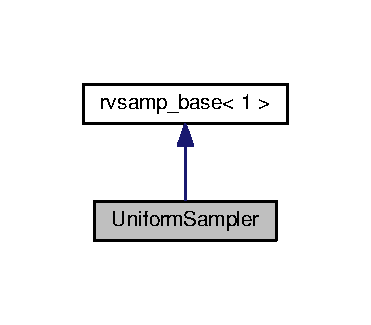
\includegraphics[width=178pt]{classUniformSampler__inherit__graph}
\end{center}
\end{figure}


Collaboration diagram for Uniform\+Sampler\+:\nopagebreak
\begin{figure}[H]
\begin{center}
\leavevmode
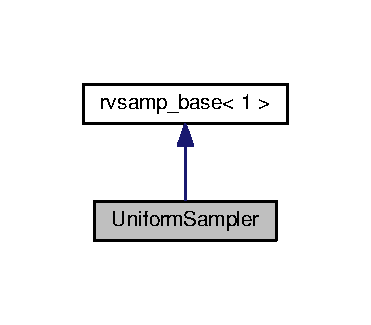
\includegraphics[width=178pt]{classUniformSampler__coll__graph}
\end{center}
\end{figure}
\subsection*{Public Member Functions}
\begin{DoxyCompactItemize}
\item 
\hyperlink{classUniformSampler_a401d133d71a0001877c3286b935fc713}{Uniform\+Sampler} ()\hypertarget{classUniformSampler_a401d133d71a0001877c3286b935fc713}{}\label{classUniformSampler_a401d133d71a0001877c3286b935fc713}

\begin{DoxyCompactList}\small\item\em The default constructor. Gives a lower bound of 0 and upper bound of 1. \end{DoxyCompactList}\item 
\hyperlink{classUniformSampler_ac2397c0d1e984c9ff4f88f25e54bb1df}{Uniform\+Sampler} (const double \&lower, const double \&upper)
\begin{DoxyCompactList}\small\item\em The constructor. \end{DoxyCompactList}\item 
double \hyperlink{classUniformSampler_a68012b943407926ea503f73daf750fe4}{sample} ()
\begin{DoxyCompactList}\small\item\em Draws a sample. \end{DoxyCompactList}\end{DoxyCompactItemize}
\subsection*{Private Attributes}
\begin{DoxyCompactItemize}
\item 
std\+::uniform\+\_\+real\+\_\+distribution \hyperlink{classUniformSampler_a4af7981a2b4e34c4bbdc6ba411f42e6e}{m\+\_\+unif\+\_\+gen}\hypertarget{classUniformSampler_a4af7981a2b4e34c4bbdc6ba411f42e6e}{}\label{classUniformSampler_a4af7981a2b4e34c4bbdc6ba411f42e6e}

\begin{DoxyCompactList}\small\item\em makes uniform random variates \end{DoxyCompactList}\end{DoxyCompactItemize}
\subsection*{Additional Inherited Members}


\subsection{Detailed Description}
A class that performs sampling from a continuous uniform distribution. 

\begin{DoxyAuthor}{Author}
taylor 
\end{DoxyAuthor}


\subsection{Constructor \& Destructor Documentation}
\index{Uniform\+Sampler@{Uniform\+Sampler}!Uniform\+Sampler@{Uniform\+Sampler}}
\index{Uniform\+Sampler@{Uniform\+Sampler}!Uniform\+Sampler@{Uniform\+Sampler}}
\subsubsection[{\texorpdfstring{Uniform\+Sampler(const double \&lower, const double \&upper)}{UniformSampler(const double &lower, const double &upper)}}]{\setlength{\rightskip}{0pt plus 5cm}Uniform\+Sampler\+::\+Uniform\+Sampler (
\begin{DoxyParamCaption}
\item[{const double \&}]{lower, }
\item[{const double \&}]{upper}
\end{DoxyParamCaption}
)}\hypertarget{classUniformSampler_ac2397c0d1e984c9ff4f88f25e54bb1df}{}\label{classUniformSampler_ac2397c0d1e984c9ff4f88f25e54bb1df}


The constructor. 


\begin{DoxyParams}{Parameters}
{\em lower} & the lower bound of the P\+R\+NG. \\
\hline
{\em upper} & the upper bound of the P\+R\+NG. \\
\hline
\end{DoxyParams}


\subsection{Member Function Documentation}
\index{Uniform\+Sampler@{Uniform\+Sampler}!sample@{sample}}
\index{sample@{sample}!Uniform\+Sampler@{Uniform\+Sampler}}
\subsubsection[{\texorpdfstring{sample()}{sample()}}]{\setlength{\rightskip}{0pt plus 5cm}double Uniform\+Sampler\+::sample (
\begin{DoxyParamCaption}
{}
\end{DoxyParamCaption}
)}\hypertarget{classUniformSampler_a68012b943407926ea503f73daf750fe4}{}\label{classUniformSampler_a68012b943407926ea503f73daf750fe4}


Draws a sample. 

\begin{DoxyReturn}{Returns}
a sample of type double. 
\end{DoxyReturn}


The documentation for this class was generated from the following file\+:\begin{DoxyCompactItemize}
\item 
include/\hyperlink{rv__samp_8h}{rv\+\_\+samp.\+h}\end{DoxyCompactItemize}

\hypertarget{classUnivNormSampler}{}\section{Univ\+Norm\+Sampler Class Reference}
\label{classUnivNormSampler}\index{Univ\+Norm\+Sampler@{Univ\+Norm\+Sampler}}


A class that performs sampling from a univariate Normal distribution.  




{\ttfamily \#include $<$rv\+\_\+samp.\+h$>$}



Inheritance diagram for Univ\+Norm\+Sampler\+:\nopagebreak
\begin{figure}[H]
\begin{center}
\leavevmode
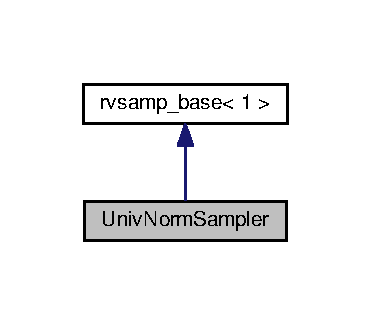
\includegraphics[width=178pt]{classUnivNormSampler__inherit__graph}
\end{center}
\end{figure}


Collaboration diagram for Univ\+Norm\+Sampler\+:\nopagebreak
\begin{figure}[H]
\begin{center}
\leavevmode
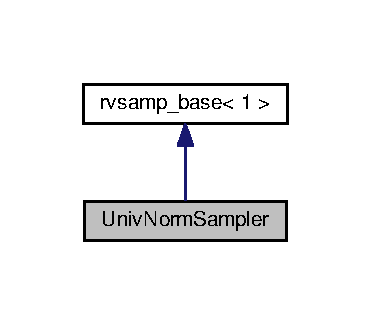
\includegraphics[width=178pt]{classUnivNormSampler__coll__graph}
\end{center}
\end{figure}
\subsection*{Public Member Functions}
\begin{DoxyCompactItemize}
\item 
\hyperlink{classUnivNormSampler_a6b751bb8877632db91266058cf6f86d9}{Univ\+Norm\+Sampler} ()\hypertarget{classUnivNormSampler_a6b751bb8877632db91266058cf6f86d9}{}\label{classUnivNormSampler_a6b751bb8877632db91266058cf6f86d9}

\begin{DoxyCompactList}\small\item\em Default-\/constructor sets up for standard Normal random variate generation. \end{DoxyCompactList}\item 
\hyperlink{classUnivNormSampler_af42cbf24a69a8888f45619bd5063a902}{Univ\+Norm\+Sampler} (const double \&mu, const double \&sigma)
\begin{DoxyCompactList}\small\item\em The user must supply both mean and std. dev. \end{DoxyCompactList}\item 
void \hyperlink{classUnivNormSampler_a9c006ba87294a3d4b2852f483bb526ce}{set\+Std\+Dev} (const double \&sigma)
\begin{DoxyCompactList}\small\item\em sets the standard deviation of the sampler. \end{DoxyCompactList}\item 
void \hyperlink{classUnivNormSampler_aea4b4a1abae5796b46aad3e70270fded}{set\+Mean} (const double \&mu)
\begin{DoxyCompactList}\small\item\em sets the mean of the sampler. \end{DoxyCompactList}\item 
double \hyperlink{classUnivNormSampler_a673c982b48f2ed65effe1751dab4ca8d}{sample} ()
\begin{DoxyCompactList}\small\item\em Draws a random number. \end{DoxyCompactList}\end{DoxyCompactItemize}
\subsection*{Private Attributes}
\begin{DoxyCompactItemize}
\item 
std\+::normal\+\_\+distribution \hyperlink{classUnivNormSampler_aa1a83f0dfcd5eb682ff09fcb6c2918b3}{m\+\_\+z\+\_\+gen}\hypertarget{classUnivNormSampler_aa1a83f0dfcd5eb682ff09fcb6c2918b3}{}\label{classUnivNormSampler_aa1a83f0dfcd5eb682ff09fcb6c2918b3}

\begin{DoxyCompactList}\small\item\em makes normal random variates \end{DoxyCompactList}\item 
double \hyperlink{classUnivNormSampler_a67db5f199eeb098ed65d461989782d1f}{m\+\_\+mu}\hypertarget{classUnivNormSampler_a67db5f199eeb098ed65d461989782d1f}{}\label{classUnivNormSampler_a67db5f199eeb098ed65d461989782d1f}

\begin{DoxyCompactList}\small\item\em the mean \end{DoxyCompactList}\item 
double \hyperlink{classUnivNormSampler_af1a2e711a4a5fded09136fd9cd161f90}{m\+\_\+sigma}\hypertarget{classUnivNormSampler_af1a2e711a4a5fded09136fd9cd161f90}{}\label{classUnivNormSampler_af1a2e711a4a5fded09136fd9cd161f90}

\begin{DoxyCompactList}\small\item\em the standard deviation \end{DoxyCompactList}\end{DoxyCompactItemize}
\subsection*{Additional Inherited Members}


\subsection{Detailed Description}
A class that performs sampling from a univariate Normal distribution. 

\begin{DoxyAuthor}{Author}
taylor 
\end{DoxyAuthor}


\subsection{Constructor \& Destructor Documentation}
\index{Univ\+Norm\+Sampler@{Univ\+Norm\+Sampler}!Univ\+Norm\+Sampler@{Univ\+Norm\+Sampler}}
\index{Univ\+Norm\+Sampler@{Univ\+Norm\+Sampler}!Univ\+Norm\+Sampler@{Univ\+Norm\+Sampler}}
\subsubsection[{\texorpdfstring{Univ\+Norm\+Sampler(const double \&mu, const double \&sigma)}{UnivNormSampler(const double &mu, const double &sigma)}}]{\setlength{\rightskip}{0pt plus 5cm}Univ\+Norm\+Sampler\+::\+Univ\+Norm\+Sampler (
\begin{DoxyParamCaption}
\item[{const double \&}]{mu, }
\item[{const double \&}]{sigma}
\end{DoxyParamCaption}
)}\hypertarget{classUnivNormSampler_af42cbf24a69a8888f45619bd5063a902}{}\label{classUnivNormSampler_af42cbf24a69a8888f45619bd5063a902}


The user must supply both mean and std. dev. 


\begin{DoxyParams}{Parameters}
{\em mu} & a double for the mean of the sampling distribution. \\
\hline
{\em sigma} & a double ($>$ 0) representing the standard deviation of the samples. \\
\hline
\end{DoxyParams}


\subsection{Member Function Documentation}
\index{Univ\+Norm\+Sampler@{Univ\+Norm\+Sampler}!sample@{sample}}
\index{sample@{sample}!Univ\+Norm\+Sampler@{Univ\+Norm\+Sampler}}
\subsubsection[{\texorpdfstring{sample()}{sample()}}]{\setlength{\rightskip}{0pt plus 5cm}double Univ\+Norm\+Sampler\+::sample (
\begin{DoxyParamCaption}
{}
\end{DoxyParamCaption}
)}\hypertarget{classUnivNormSampler_a673c982b48f2ed65effe1751dab4ca8d}{}\label{classUnivNormSampler_a673c982b48f2ed65effe1751dab4ca8d}


Draws a random number. 

\begin{DoxyReturn}{Returns}
a random sample of type double. 
\end{DoxyReturn}
\index{Univ\+Norm\+Sampler@{Univ\+Norm\+Sampler}!set\+Mean@{set\+Mean}}
\index{set\+Mean@{set\+Mean}!Univ\+Norm\+Sampler@{Univ\+Norm\+Sampler}}
\subsubsection[{\texorpdfstring{set\+Mean(const double \&mu)}{setMean(const double &mu)}}]{\setlength{\rightskip}{0pt plus 5cm}void Univ\+Norm\+Sampler\+::set\+Mean (
\begin{DoxyParamCaption}
\item[{const double \&}]{mu}
\end{DoxyParamCaption}
)}\hypertarget{classUnivNormSampler_aea4b4a1abae5796b46aad3e70270fded}{}\label{classUnivNormSampler_aea4b4a1abae5796b46aad3e70270fded}


sets the mean of the sampler. 


\begin{DoxyParams}{Parameters}
{\em mu} & the desired mean. \\
\hline
\end{DoxyParams}
\index{Univ\+Norm\+Sampler@{Univ\+Norm\+Sampler}!set\+Std\+Dev@{set\+Std\+Dev}}
\index{set\+Std\+Dev@{set\+Std\+Dev}!Univ\+Norm\+Sampler@{Univ\+Norm\+Sampler}}
\subsubsection[{\texorpdfstring{set\+Std\+Dev(const double \&sigma)}{setStdDev(const double &sigma)}}]{\setlength{\rightskip}{0pt plus 5cm}void Univ\+Norm\+Sampler\+::set\+Std\+Dev (
\begin{DoxyParamCaption}
\item[{const double \&}]{sigma}
\end{DoxyParamCaption}
)}\hypertarget{classUnivNormSampler_a9c006ba87294a3d4b2852f483bb526ce}{}\label{classUnivNormSampler_a9c006ba87294a3d4b2852f483bb526ce}


sets the standard deviation of the sampler. 


\begin{DoxyParams}{Parameters}
{\em sigma} & the desired standard deviation. \\
\hline
\end{DoxyParams}


The documentation for this class was generated from the following file\+:\begin{DoxyCompactItemize}
\item 
include/\hyperlink{rv__samp_8h}{rv\+\_\+samp.\+h}\end{DoxyCompactItemize}

\chapter{File Documentation}
\hypertarget{auxiliary__pf_8h}{}\section{include/auxiliary\+\_\+pf.h File Reference}
\label{auxiliary__pf_8h}\index{include/auxiliary\+\_\+pf.\+h@{include/auxiliary\+\_\+pf.\+h}}


A base class for Auxiliary Particle Filtering. Inherit from this if you want to use an \hyperlink{classAPF}{A\+PF} for your state space model. Filtering only, no smoothing.  


{\ttfamily \#include $<$array$>$}\\*
{\ttfamily \#include $<$functional$>$}\\*
{\ttfamily \#include $<$Eigen/\+Dense$>$}\\*
{\ttfamily \#include $<$cmath$>$}\\*
{\ttfamily \#include \char`\"{}rv\+\_\+samp.\+h\char`\"{}}\\*
{\ttfamily \#include $<$iostream$>$}\\*
Include dependency graph for auxiliary\+\_\+pf.\+h\+:
\nopagebreak
\begin{figure}[H]
\begin{center}
\leavevmode
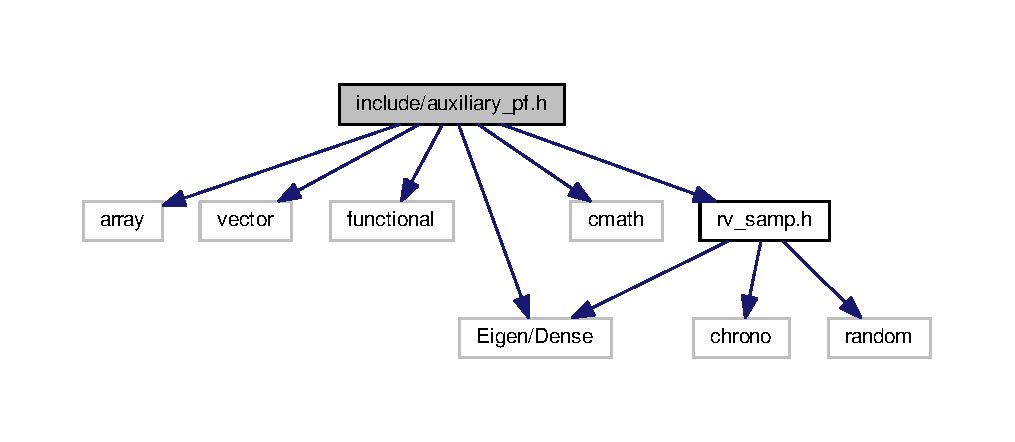
\includegraphics[width=350pt]{auxiliary__pf_8h__incl}
\end{center}
\end{figure}
\subsection*{Classes}
\begin{DoxyCompactItemize}
\item 
class \hyperlink{classAPF}{A\+P\+F$<$ nparts, dimx, dimy, resamp\+T $>$}
\begin{DoxyCompactList}\small\item\em A base-\/class for Auxiliary Particle Filtering. Filtering only, no smoothing. \end{DoxyCompactList}\end{DoxyCompactItemize}


\subsection{Detailed Description}
A base class for Auxiliary Particle Filtering. Inherit from this if you want to use an \hyperlink{classAPF}{A\+PF} for your state space model. Filtering only, no smoothing. 


\begin{DoxyTemplParams}{Template Parameters}
{\em nparts} & the number of particles \\
\hline
{\em dimx} & the dimension of the state \\
\hline
{\em dimy} & the dimension of the observations \\
\hline
{\em resampT} & the resampler type \\
\hline
\end{DoxyTemplParams}

\hypertarget{bootstrap__filter_8h}{}\section{include/pf/bootstrap\+\_\+filter.h File Reference}
\label{bootstrap__filter_8h}\index{include/pf/bootstrap\+\_\+filter.\+h@{include/pf/bootstrap\+\_\+filter.\+h}}


bootstrap particle filter  


{\ttfamily \#include $<$array$>$}\newline
{\ttfamily \#include $<$vector$>$}\newline
{\ttfamily \#include $<$Eigen/\+Dense$>$}\newline
{\ttfamily \#include \char`\"{}pf\+\_\+base.\+h\char`\"{}}\newline
Include dependency graph for bootstrap\+\_\+filter.\+h\+:\nopagebreak
\begin{figure}[H]
\begin{center}
\leavevmode
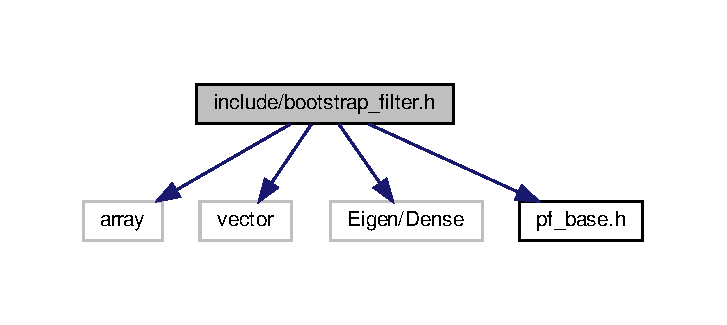
\includegraphics[width=350pt]{bootstrap__filter_8h__incl}
\end{center}
\end{figure}
\subsection*{Classes}
\begin{DoxyCompactItemize}
\item 
class \hyperlink{classBSFilter}{B\+S\+Filter$<$ nparts, dimx, dimy, resamp\+\_\+t, float\+\_\+t, debug $>$}
\begin{DoxyCompactList}\small\item\em A base class for the bootstrap particle filter. \end{DoxyCompactList}\end{DoxyCompactItemize}


\subsection{Detailed Description}
bootstrap particle filter 


\begin{DoxyTemplParams}{Template Parameters}
{\em nparts} & the number of particles \\
\hline
{\em dimx} & the dimension of the state \\
\hline
{\em dimy} & the dimension of the observations \\
\hline
{\em resamp\+\_\+t} & the type of resampler \\
\hline
\end{DoxyTemplParams}

\hypertarget{resamplers_8h}{}\section{include/pf/resamplers.h File Reference}
\label{resamplers_8h}\index{include/pf/resamplers.\+h@{include/pf/resamplers.\+h}}


all resamplers must inherit from this. This will enforce certain structure that are assumed by all particle filters.  


{\ttfamily \#include $<$chrono$>$}\newline
{\ttfamily \#include $<$array$>$}\newline
{\ttfamily \#include $<$random$>$}\newline
{\ttfamily \#include $<$numeric$>$}\newline
{\ttfamily \#include $<$cmath$>$}\newline
{\ttfamily \#include $<$Eigen/\+Dense$>$}\newline
Include dependency graph for resamplers.\+h\+:
\nopagebreak
\begin{figure}[H]
\begin{center}
\leavevmode
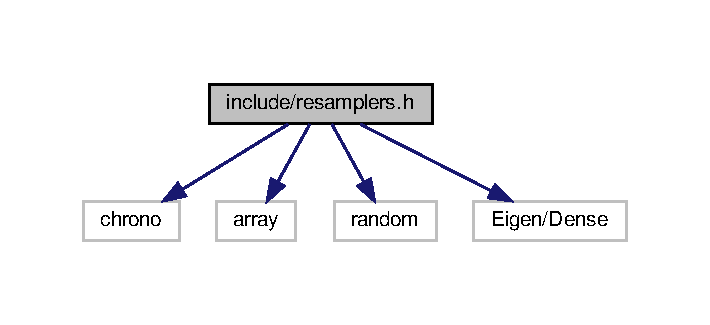
\includegraphics[width=350pt]{resamplers_8h__incl}
\end{center}
\end{figure}
\subsection*{Classes}
\begin{DoxyCompactItemize}
\item 
class \hyperlink{classrbase}{rbase$<$ nparts, dimx, float\+\_\+t $>$}
\begin{DoxyCompactList}\small\item\em Base class for all resampler types. \end{DoxyCompactList}\item 
class \hyperlink{classmn__resampler}{mn\+\_\+resampler$<$ nparts, dimx, float\+\_\+t $>$}
\item 
class \hyperlink{classmn__resampler__rbpf}{mn\+\_\+resampler\+\_\+rbpf$<$ nparts, dimsampledx, cf\+Mod\+T, float\+\_\+t $>$}
\item 
class \hyperlink{classresid__resampler}{resid\+\_\+resampler$<$ nparts, dimx, float\+\_\+t $>$}
\item 
class \hyperlink{classstratif__resampler}{stratif\+\_\+resampler$<$ nparts, dimx, float\+\_\+t $>$}
\item 
class \hyperlink{classsystematic__resampler}{systematic\+\_\+resampler$<$ nparts, dimx, float\+\_\+t $>$}
\item 
class \hyperlink{classmn__resamp__fast1}{mn\+\_\+resamp\+\_\+fast1$<$ nparts, dimx, float\+\_\+t $>$}
\end{DoxyCompactItemize}


\subsection{Detailed Description}
all resamplers must inherit from this. This will enforce certain structure that are assumed by all particle filters. 

Class that performs multinomial resampling for \char`\"{}standard\char`\"{} models. For justification, see page 244 of \char`\"{}\+Inference in Hidden Markov Models\char`\"{}.

Class that performs systematic resampling on \char`\"{}standard\char`\"{} models.

Class that performs stratified resampling on \char`\"{}standard\char`\"{} models.

Class that performs residual resampling on \char`\"{}standard\char`\"{} models.

Class that performs multinomial resampling for R\+B\+P\+Fs.

Class that performs multinomial resampling for \char`\"{}standard\char`\"{} models.


\begin{DoxyTemplParams}{Template Parameters}
{\em nparts} & the number of particles. \\
\hline
{\em dimx} & the dimension of each state sample.\\
\hline
{\em nparts} & the number of particles. \\
\hline
{\em dimsampledx} & the dimension of each state sample. \\
\hline
{\em cf\+ModT} & the type of closed form model \\
\hline
{\em float\+\_\+t} & the type of floating point number\\
\hline
{\em nparts} & the number of particles. \\
\hline
{\em dimx} & the dimension of each state sample. \\
\hline
{\em float\+\_\+t} & the floating point for samples \\
\hline
\end{DoxyTemplParams}

\hypertarget{rv__samp_8h}{}\section{include/pf/rv\+\_\+samp.h File Reference}
\label{rv__samp_8h}\index{include/pf/rv\+\_\+samp.\+h@{include/pf/rv\+\_\+samp.\+h}}


all rv samplers must inherit from this.  


{\ttfamily \#include $<$chrono$>$}\newline
{\ttfamily \#include $<$Eigen/\+Dense$>$}\newline
{\ttfamily \#include $<$random$>$}\newline
Include dependency graph for rv\+\_\+samp.\+h\+:
\nopagebreak
\begin{figure}[H]
\begin{center}
\leavevmode
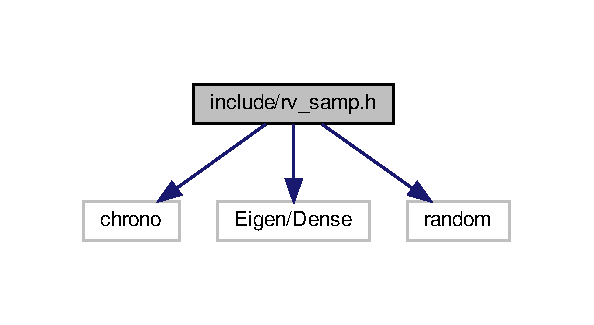
\includegraphics[width=285pt]{rv__samp_8h__incl}
\end{center}
\end{figure}
This graph shows which files directly or indirectly include this file\+:
\nopagebreak
\begin{figure}[H]
\begin{center}
\leavevmode
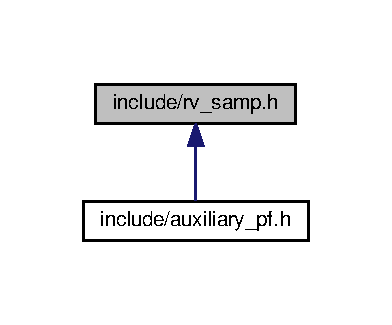
\includegraphics[width=199pt]{rv__samp_8h__dep__incl}
\end{center}
\end{figure}
\subsection*{Classes}
\begin{DoxyCompactItemize}
\item 
class \hyperlink{classrvsamp_1_1rvsamp__base}{rvsamp\+::rvsamp\+\_\+base}
\begin{DoxyCompactList}\small\item\em Base class for all random variable sampler types. Primary benefit is that it sets the seed for you. \end{DoxyCompactList}\item 
class \hyperlink{classrvsamp_1_1UnivNormSampler}{rvsamp\+::\+Univ\+Norm\+Sampler$<$ float\+\_\+t $>$}
\begin{DoxyCompactList}\small\item\em A class that performs sampling from a univariate Normal distribution. \end{DoxyCompactList}\item 
class \hyperlink{classrvsamp_1_1UnivLogNormSampler}{rvsamp\+::\+Univ\+Log\+Norm\+Sampler$<$ float\+\_\+t $>$}
\begin{DoxyCompactList}\small\item\em A class that performs sampling from a univariate Log-\/\+Normal distribution. \end{DoxyCompactList}\item 
class \hyperlink{classrvsamp_1_1UnivGammaSampler}{rvsamp\+::\+Univ\+Gamma\+Sampler$<$ float\+\_\+t $>$}
\begin{DoxyCompactList}\small\item\em A class that performs sampling from a univariate Gamma distribution. \end{DoxyCompactList}\item 
class \hyperlink{classrvsamp_1_1UnivInvGammaSampler}{rvsamp\+::\+Univ\+Inv\+Gamma\+Sampler$<$ float\+\_\+t $>$}
\begin{DoxyCompactList}\small\item\em A class that performs sampling from a univariate Inverse Gamma distribution. \end{DoxyCompactList}\item 
class \hyperlink{classrvsamp_1_1TruncUnivNormSampler}{rvsamp\+::\+Trunc\+Univ\+Norm\+Sampler$<$ float\+\_\+t $>$}
\begin{DoxyCompactList}\small\item\em A class that performs sampling from a truncated univariate Normal distribution. \end{DoxyCompactList}\item 
class \hyperlink{classrvsamp_1_1PoissonSampler}{rvsamp\+::\+Poisson\+Sampler$<$ float\+\_\+t, int\+\_\+t $>$}
\begin{DoxyCompactList}\small\item\em A class that performs sampling from a Poisson distribution. \end{DoxyCompactList}\item 
class \hyperlink{classrvsamp_1_1BernSampler}{rvsamp\+::\+Bern\+Sampler$<$ float\+\_\+t, int\+\_\+t $>$}
\begin{DoxyCompactList}\small\item\em A class that performs sampling from a univariate Bernoulli distribution. \end{DoxyCompactList}\item 
class \hyperlink{classrvsamp_1_1MVNSampler}{rvsamp\+::\+M\+V\+N\+Sampler$<$ dim, float\+\_\+t $>$}
\begin{DoxyCompactList}\small\item\em A class that performs sampling from a multivariate normal distribution. \end{DoxyCompactList}\item 
class \hyperlink{classrvsamp_1_1UniformSampler}{rvsamp\+::\+Uniform\+Sampler$<$ float\+\_\+t $>$}
\begin{DoxyCompactList}\small\item\em A class that performs sampling from a continuous uniform distribution. \end{DoxyCompactList}\item 
class \hyperlink{classrvsamp_1_1k__gen}{rvsamp\+::k\+\_\+gen$<$ N, float\+\_\+t $>$}
\begin{DoxyCompactList}\small\item\em A class that performs sampling with replacement (useful for the index sampler in an \hyperlink{classAPF}{A\+PF}) \end{DoxyCompactList}\end{DoxyCompactItemize}


\subsection{Detailed Description}
all rv samplers must inherit from this. 

Basically a wrapper for std\+::discrete\+\_\+distribution$<$$>$ outputs are in the rage (0,1,...N-\/1)

Can sample from a distribution with fixed mean and covariance, fixed mean only, fixed covariance only, or nothing fixed.

Samples from univariate Bernoulli distribution.

Samples from univariate Poisson distribution.

Samples from a truncated univariate Normal distribution using the acceptance rejection method. The proposal distribution used is a normal distribution with the same location and scale parameters as the target. As a result, this method will take a long time when the width of the support of the target is narrow.

Samples from univariate Inverse Gamma distribution.

Samples from univariate Gamma distribution.

Samples from univariate Log-\/\+Normal distribution.

Samples from univariate Normal distribution.


\begin{DoxyTemplParams}{Template Parameters}
{\em dim} & the dimension of each random vector sample.\\
\hline
\end{DoxyTemplParams}

\hypertarget{sisr__filter_8h}{}\section{include/pf/sisr\+\_\+filter.h File Reference}
\label{sisr__filter_8h}\index{include/pf/sisr\+\_\+filter.\+h@{include/pf/sisr\+\_\+filter.\+h}}


S\+I\+SR filter.  


{\ttfamily \#include $<$array$>$}\newline
{\ttfamily \#include $<$Eigen/\+Dense$>$}\newline
{\ttfamily \#include \char`\"{}pf\+\_\+base.\+h\char`\"{}}\newline
Include dependency graph for sisr\+\_\+filter.\+h\+:\nopagebreak
\begin{figure}[H]
\begin{center}
\leavevmode
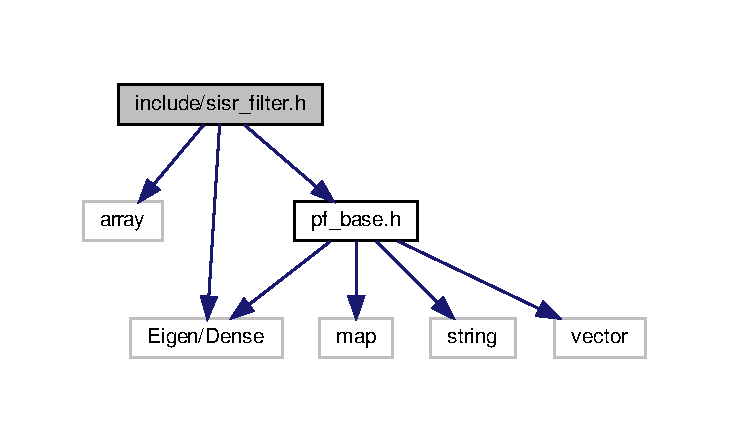
\includegraphics[width=350pt]{sisr__filter_8h__incl}
\end{center}
\end{figure}
\subsection*{Classes}
\begin{DoxyCompactItemize}
\item 
class \hyperlink{classSISRFilter}{S\+I\+S\+R\+Filter$<$ nparts, dimx, dimy, resamp\+\_\+t, float\+\_\+t, debug $>$}
\begin{DoxyCompactList}\small\item\em A base class for the Sequential Important Sampling with Resampling (S\+I\+SR). \end{DoxyCompactList}\end{DoxyCompactItemize}


\subsection{Detailed Description}
S\+I\+SR filter. 


\begin{DoxyTemplParams}{Template Parameters}
{\em nparts} & the number of particles \\
\hline
{\em dimx} & the size of the state \\
\hline
{\em the} & size of the observation \\
\hline
{\em resamp\+\_\+t} & the type of resampler \\
\hline
\end{DoxyTemplParams}

%--- End generated contents ---

% Index
\backmatter
\newpage
\phantomsection
\clearemptydoublepage
\addcontentsline{toc}{chapter}{Index}
\printindex

\end{document}
